\documentclass[hyperref,UTF8,12pt]{article}

\usepackage[leqno]{amsmath}
\usepackage{amssymb}
\usepackage{amsthm}
\usepackage{bm}
\usepackage{indentfirst}
 \usepackage[backref]{hyperref}
 \usepackage{mathpazo}
%\usepackage{cite}
\usepackage{extarrows}
\hypersetup{%
	colorlinks = true,
	linkcolor  = black
}
\usepackage{setspace}
\linespread{1.1}
\renewcommand{\arraystretch}{1.3}
\usepackage{mathtools}
\makeatletter
\newcommand{\leqnomode}{\tagsleft@true}
\newcommand{\reqnomode}{\tagsleft@false}
\makeatother
\usepackage{geometry}
\usepackage{tikz-cd}
\usepackage{color}
\usepackage[title]{appendix}
\usepackage[T1]{fontenc}
\usepackage{hhline}
%\usepackage{diagbox}
%\newcommand{\emptydiag}[2][]{
%\diagbox[innerwidth=\widthof{#2},height=\line]{}{}
%}

\numberwithin{equation}{subsection}

\theoremstyle{plain}
\newtheorem{theorem}{Theorem}
\newtheorem{lemma}{Lemma}
\newtheorem{proposition}{Proposition}
\newtheorem{corollary}{Corollary}
\newtheorem{definition}{Definition}

\theoremstyle{definition}
\newtheorem{remark}{Remark}
\newtheorem{problem}{Problem}
\newtheorem{example}{Example}

\numberwithin{theorem}{section}
\numberwithin{lemma}{section}
\numberwithin{proposition}{section}
\numberwithin{remark}{section}
\numberwithin{corollary}{section}
\numberwithin{definition}{section}
\numberwithin{problem}{section}
\numberwithin{example}{section}

\allowdisplaybreaks

\def\e{\textup{e}}
\def\i{\textup{i}}
\def\dif{\textup{d}}
\def\T{\textup{T}}
\def\diag{\textup{diag}}
\def\id{\textup{id}}
\def\dv{\textup{div}}
\def\hess{\textup{Hess}}
%下面是一些数学命令的简化
\def\Xint#1{\mathchoice
	{\XXint\displaystyle\textstyle{#1}}%
	{\XXint\textstyle\scriptstyle{#1}}%
	{\XXint\scriptstyle\scriptscriptstyle{#1}}%
	{\XXint\scriptscriptstyle\scriptscriptstyle{#1}}%
	\!\int}
\def\XXint#1#2#3{{\setbox0=\hbox{$#1{#2#3}{\int}$ }
		\vcenter{\hbox{$#2#3$ }}\kern-.55\wd0}}
\def\ddashint{\Xint=}
\def\dashint{\Xint-}
\newcommand{\SUM}[1]{\displaystyle\sum_{#1}^\infty}
\newcommand{\chfrac}[2]{\dfrac{\:#1\:}{\:#2\:}}
\newcommand{\exer}[1]{\noindent\textbf{#1}}
\newcommand{\sssec}[1]{\noindent\textbf{\color{fcolor}{#1}}}
\newcommand{\toi}[1]{{#1}\to\infty}
\newcommand{\dis}{\displaystyle}
\newcommand{\limls}{\lim\limits}
\newcommand{\ptl}{\partial}
%\newcommand{\bv}{\mathrm{BV}}
%\newcommand{\ac}{\mathrm{AC}}
\newcommand{\mr}{\mathbb{R}}
\newcommand{\mn}{\mathbb{N}}
\newcommand{\mq}{\mathbb{Q}}
\newcommand{\mz}{\mathbb{Z}}
\newcommand{\mc}{\mathbb{C}}
\newcommand{\rel}{\text{ rel }}
\renewcommand{\leq}{\leqslant}
\renewcommand{\geq}{\geqslant}
%\renewcommand{\hom}{\operatorname{Hom}}
%\renewcommand{\ker}{\operatorname{ker}}
%\newcommand{\obj}{\operatorname{obj}}
\newcommand{\tr}{\operatorname{tr}}
\newcommand{\divv}{\operatorname{div}}
\newcommand{\curl}{\operatorname{curl}}
\newcommand{\spt}{\operatorname{spt}}
\newcommand{\ve}{\varepsilon}
\newcommand{\bs}{\backslash}
\newcommand{\re}{\operatorname{Re}}
\newcommand{\im}{\operatorname{im}}
\newcommand{\ima}{\operatorname{Im}}
%\newcommand{\coker}{\operatorname{coker}}
%\newcommand{\slfrac}[2]{\left.#1\middle/#2\right.}
%\newcommand{\noun}[1]{\noindent\textbf{#1}\quad}
\newcommand{\intr}{\operatorname{Int}}
%\newcommand{\lesim}{\mathrel{\underset{\rotatebox{-15}{$\sim$}}{<}}}
\geometry{a4paper,left=2.2cm,right=2.2cm,top=2cm,bottom=2cm}
\hypersetup{colorlinks=true }

\title{Notes on Partial Differential Equations}
\author{H\textsc{arvey}\ P\textsc{eng}}
 \begin{document}

\maketitle
\begin{abstract}
This note is based on lectures by Prof. Xu Guixiang in 2023 fall. This is a selection and expansion of the involved content of \textit{Partial Differential Equations} by Evans, but is not endorsed by the lecturer. All errors are almost surely mine, and I'd be very grateful if you could send an email to \href{mailto:3275779330@qq.com}{3275779330@qq.com} to point them out.
\end{abstract} 

\tableofcontents
\newpage 
\section{Introduction}

This course is an introduction to the mathematical study of Partial Differential
Equations(PDEs), which are ubiquitous in mathematically oriented scientific fields, such as physics(where people use PDEs to study sound, heat, diffusion, and quantum mechanics, etc.) and engineering(structural mechanics, image processing, for example). The course will mainly cover four prototype linear equations and a transform method - Fourier transform, but will not focus on modern functional analytic techniques.

We will of course meet several specific equations, but we do NOT "just solve" them. In general, given a system of PDE, there are several questions we can ask:
\begin{itemize}
	\item Does a solution exist?
	\item Is the solution unique?
	\item Does the solution depend continuously on the data, such as the desired values of the solution on the boundary of our domain, or the
	starting configuration when there is a time variable?
	\item How \textit{regular} is the solution? Is it continuously differentiable? Or even
	smooth?
\end{itemize}


Before we define what a partial differential equation is, I recommend that, if you are new to PDE, you should read the appendix now, where you could find notations and important analytic tools used. Note that we write "PDE" as an abbreviation for both the singular "partial differential equation" and the plural "partial differential equations".

In summary, a PDE is an equation involving an unknown function of two or more variables and certain of its partial derivatives. Fix an integer $k\geq1$.
\begin{definition}
A \emph{partial differential equation} of \emph{order} $k$ is an expression of the form
\begin{equation}
\label{1st}\tag{1}F(D^ku(x),D^{k-1}u(x),\cdots,Du(x),u(x),x)=0,
\end{equation}
where $F:\mr^{n^k}\times\mr^{n^{k-1}}\times\cdots\times\mr^n\times\mr\times U \to\mr$ is given, and $u:U\to\mr$ is the unknown.
\end{definition}
We now try to crudely classify (\ref{1st}), and after that we shall present some examples of each class.
\begin{definition}
\textup{(i)} The partial differential equation \textup{(\ref{1st})} is called \emph{linear} if it has the form
\[\sum_{|\alpha|\leq k}a_\alpha(x)D^\alpha u=f(x)\]
for given functions $a_\alpha(|\alpha|\leq k), f$. This linear PDE is \emph{homogeneous} if $f \equiv 0$.\\
\textup{(ii)} The PDE \textup{(\ref{1st})} is \emph{semilinear} if it has the form
\[\sum_{|\alpha|=k}a_\alpha(x)D^\alpha u+a_0(D^{k-1}u,\cdots,Du,u,x)=0.\]
\textup{(iii)} The PDE \textup{(\ref{1st})} is \emph{quasilinear} if it has the form\[
\sum_{|\alpha|=k}a_\alpha(D^{k-1}u,\cdots,Du,u,x)D^\alpha u+a_0(D^{k-1}u,\cdots,Du,u,x)=0.\]
\textup{(iv)} The PDE \textup{(\ref{1st})} is \emph{fully nonlinear} if it depends nonlinearly upon the highest order derivatives.
\end{definition}
\begin{definition}
A \emph{system of partial differential equation} of \emph{order} $k$ is an expression of the form
\begin{equation}
	\label{2nd}\tag{2}\mathbf{F}(D^k\mathbf{u}(x),D^{k-1}\mathbf{u}(x),\cdots,D\mathbf{u}(x),\mathbf{u}(x),x)=0,
\end{equation}
where $\mathbf{F}:\mr^{mn^k}\times\mr^{mn^{k-1}}\times\cdots\times\mr^{mn}\times\mr^m\times U\to\mr^m$ is given, and $\mathbf{u}:U\to\mr^m,\mathbf{u}=(u^1,\cdots,u^m)$ is the unknown.
\end{definition}
Systems are classified in the obvious way as being linear, semilinear, etc.

There is no general theory known concerning the solvability of all partial differential equations. Instead, research focuses on various particular partial differential equations that are important for applications, and following is a list of many specific partial differential equations of interest in current research. The ones that appears in the following sections won't be listed.
\begin{enumerate}
	\item Single partial differential equations.
	\begin{enumerate}
		\item Linear equations.
		\begin{enumerate}
			\item Helmholtz's (or eigenvalue) equation\[-\Delta u=\lambda u.\]
			\item Liouville's equation\[u_t-\sum_{i=1}^n(b^iu)_{x_i}=0.\]
			\item Telegraph equation\[u_{tt}+2du_t-u_{xx}=0.\]
			\item Airy's equation\[u_t+u_{xxx}=0.\]
		\end{enumerate}
		\item Nonlinear equations.
		\begin{enumerate}
			\item Eikonal equation\[|Du|=1.\]
			\item $p$-Laplacian equation
			\[\divv(|Du|^{p-2}Du)=0.\]
			\item Minimal surface equation
			\[\divv\left(\frac{Du}{(1+|Du|^2)^{1/2}}\right)=0.\]
			\item Korteweg-de Vries (KdV) equation\[u_t+uu_x+u_{xxx}=0.\]
		\end{enumerate}
	\end{enumerate}
	\item Systems of partial differential equations.
	\begin{enumerate}
		\item Linear systems.
		\begin{enumerate}
			\item Equilibrium equations of linear elasticity
			\[\mu\Delta\mathbf{u}+(\lambda+\mu) D(\divv\mathbf{u})=\mathbf{0}.\]
			\item Maxwell's equations\[\begin{cases}
				\mathbf{E}_t=\curl\mathbf{B}\\
				\mathbf{B}_t=-\curl\mathbf{E}\\
				\divv\mathbf{B}=\divv\mathbf{E}=0.
			\end{cases}\]
		\end{enumerate}
		\item Nonlinear systems.
		\begin{enumerate}
			\item System of conservation laws
			\[\mathbf{u}_t+\divv\mathbf{F}(\mathbf{u})=\mathbf{0}.\]
			\item Navier-Stokes equations for incompressible, viscous flow\[\begin{cases}
			\mathbf{u}_t+\mathbf{u}\cdot D\mathbf{u}-\Delta\mathbf{u}=-Dp\\
			\divv\mathbf{u}=0.
			\end{cases}\]
		\end{enumerate}
	\end{enumerate}
\end{enumerate}
Enlightened from the questions raised before, we say that a given problem for a PDE is \emph{well-posed} if
\begin{enumerate}
	\item the problem in fact has a solution;
	\item this solution is unique;
	\item the solution depends continuously on the data given in the problem.
\end{enumerate}
Now it's time to clarify what a solution actually is. We clearly want the solution to have certain properties, for example, real analytic. But is it too much? Maybe it would be wiser to require a solution of a PDE of order $k$ to be at least $k$ times continuously differentiable.
\begin{definition}
We say $u \in C^k(U)$ is \emph{classical solution} of a PDE if in fact the PDE is identically satisfied on $U$ when $u,Du,\cdots,D^k u$ are substituted in.
\end{definition}
However, for many PDE, we cannot achieve this. Under many circumstances we must allow for solutions $u$ which are not continuously differentiable or even continuous. In general, these equations has no classical solutions but is well-posed if we allow for properly defined \emph{generalized} or \emph{weak solutions}.

The point is this: if from the outset we demand that our solutions be very regular, say $k$-times continuously differentiable, then it is usually hard to find them; a far more reasonable strategy is to consider as separate the \emph{existence} and the \emph{smoothness} (or \emph{regularity}) problems. But let me explicitly note here that Part I is mainly devoted to deriving formulas for the classical solutions. After that the book starts spending efforts on proving mathematically the existence of solutions to various sorts of partial differential equations.

\newpage
\section{Four Important Linear PDE}
In this chapter we introduce four fundamental linear partial differential equations for which various explicit formulas for solutions are available. These are
\[\begin{aligned}
	&\text{the transport equation}\quad &u_t+b\cdot Du=0\quad &(\S 2.1),\\
	&\text{Laplace's equation}\quad &\Delta u=0\quad &(\S 2.2),\\
	&\text{the heat equation}\quad &u_t-\Delta u=0\quad &(\S 2.3),\\
	&\text{the wave equation}\quad &u_{tt}-\Delta u=0\quad &(\S 2.4).
\end{aligned}\]
Before going further, the reader is again advised to review the discussions of integration by parts, Green's formulas, convolutions, etc., in the appendix and later refer back to these as necessary.

\subsection{Transport equation}
One of the simplest partial differential equations is{\color{red}\[u_t+b\cdot Du=0\quad\text{in}~\mr^n\times(0,\infty),\tag{1}\]}where $b=(b_1,\cdots,b_n)$ is a fixed vector in $\mr^n$, and $u=u(x,t):\mr^n\times[0,\infty)\to\mr$ is the unknown.\\
\textcolor{blue}{Homogeneous problem.} Our aim is to solve the initial-value problem\[\tag{2}\begin{cases}
	\hfill u_t+b\cdot Du=0\quad&\text{in}~\mr^n\times(0,\infty)\\
	\hfill u=g\quad&\text{on}~\mr^n\times\{t=0\}.
\end{cases}\] Fix any point $(x,t)\in\mr^n\times(0,\infty)$ and define $z(s):=u(x+sb,t+s)(s\in\mr)$. We then calculate \[z^\prime(s)=Du(x+sb,t+s)\cdot b+u_t(x+sb,t+s)=0,\]implying that $z(s)$ is constant on the line through $(x,t)$ with the direction $(b,1)\in\mr^{n+1}$. Note that this line hit the plane $\mr^n\times\{t=0\}$ when $s=-t$, at the point $(x-tb,0)$, thus $z(-t)=u(x-tb,0)=g(x-tb)$. Since $u$ is constant on the line, we conclude that $u(x,t)=g(x-tb)$.\\
\textcolor{blue}{Nonhomogeneous problem.} Now we turn to \[\label{transNon}\tag{3}\begin{cases}
	\hfill u_t+b\cdot Du=f\quad&\text{in}~\mr^n\times(0,\infty)\\
	\hfill u=g\quad&\text{on}~\mr^n\times\{t=0\}.
\end{cases}\]Fix $(x,t)$ and define $z(s)$ as before, and this time we have $z^\prime(s)=f(x+s b,t+s)$. Consequently\[\begin{aligned}
&u(x,t)-g(x-tb)=z(0)-z(-t)=\int_{-t}^0z^\prime(s)\dif s \\
=&\int_{-t}^0f(x+sb,t+s)\dif s=\int_0^tf(x+(s-t)b,s)\dif s
\end{aligned}\]and so\[\tag{4}u(x,t)=g(x-tb)+\int_0^tf(x+(s-t)b,s)\dif s\quad(x\in\mr^n,t\geq0)\]solves (\ref{transNon}).

\subsection{Laplace's equation}
In this section we will study a very important example of elliptic PDE - Laplace's equation{\color{red}\[\Delta u=0\tag{5}\label{Laplace1}\]}and its generalization - Poisson's equation{\color{red}\[-\Delta u=f.\tag{6}\label{Laplace2}\]}In both (\ref{Laplace1}) and (\ref{Laplace2}), $x\in U$ and the unknown is $u:\bar{U}\to\mr,u=u(x)$. In (\ref{Laplace2}) the function $f:U\to\mr$ is also given.
\begin{definition}
A $C^2$ function $u$ satisfying \textup{(\ref{Laplace1})} is called a \emph{harmonic} function.
\end{definition}
\noindent\textcolor{blue}{Fundamental solution.} Laplace's equation is invariant under rotation(Problem \ref{prob2}), so we first find radial solutions. Set $v(r)=u(x)$ where $r=|x|=(x_1^2+\cdots+x_n^2)^{1/2}$. First we calculate $\dfrac{\ptl r}{\ptl x_i}= \dfrac{1}{2}(x_1^2+\cdots+x_n^2)^{-1/2}\cdot2x_i=\dfrac{x_i}{r}(1\leq i\leq n,x\neq0)$, and so\[u_{x_i}=v^\prime(r)\frac{\ptl r}{\ptl x_i}=\frac{x_i}{r}v^\prime(r), u_{x_ix_i}=\ptl_{x_i}\frac{x_i}{r}v^\prime(r)+\frac{x_i}{r}v^{\prime\prime}(r)\ptl_{x_i}r=\frac{r^2-x_i^2}{r^3}v^\prime(r)+\frac{x_i^2}{r^2}v^{\prime\prime}(r).\]Hence\[
\Delta u=\frac{n}{r}v^\prime(r)-\frac{x_1^2+\cdots+x_n^2}{r^3}v^\prime(r)+ \frac{x_1^2+\cdots+x_n^2}{r^2}v^{\prime\prime}(r)=v^{\prime\prime}(r)+\frac{n-1}{r}v^\prime(r).\]Since $u$ solves (\ref{Laplace1}), we have $\dfrac{v^{\prime\prime}(r)}{v^\prime(r)}=\dfrac{1-n}{r}$ if $v^\prime\neq0$. We deduce $\ln(|v^\prime|)^\prime=\dfrac{v^{\prime\prime}}{v^\prime}=\dfrac{1-n}{r}$, and thus $v^\prime(r)=Cr^{1-n}$ for some constant $C$. Integrate again to obtain \[v(r)=\begin{cases}
	C\ln r+C_1,&n=2\\\frac{Cr^{2-n}}{2-n}+C_2,&n\geq3.
\end{cases}\]Therefore, if we choose "appropriate" constants, we get the following
\begin{definition}
The function
\[\Phi(x):=\begin{cases}-\frac{1}{2\pi}\ln|x|,&n=2\\ \frac{1}{n(n-2)\alpha(n)} \frac{1}{|x|^{n-2}},&n\geq3,\end{cases}\tag{7}\]
defined for $x\in\mr^n,x\neq0$, is the \emph{fundamental solution} of \textup{(\ref{Laplace1})}.
\end{definition}
\noindent\textcolor{blue}{Basic estimates.} We have \[\tag{8}\label{8}
|D\Phi(x)|\leq\frac{C}{|x|^{n-1}},|D^2\Phi(x)|\leq\frac{C}{|x|^n}(x\neq0).\]This is obvious from direct computations of $D\Phi(x)$ and $D^2\Phi(x)$, omitting the constants.

\noindent\textcolor{blue}{Poisson's equation.} The basic idea is as follows:\[\begin{gathered}
x\mapsto\Phi(x)~\text{is harmonic}\xRightarrow{\text{shift}}\Phi(x-y)~\text{also harmonic as a function of }x\xRightarrow{\text{multiplication}}\\ \Phi(x-y)f(y)~\text{also harmonic}\xRightarrow{\text{sum with respect to }y}\int_{\mr^n}\Phi(x-y)f(y)\dif y~\text{is also harmonic}.
\end{gathered}\]But this is WRONG because $D^2\Phi(x-y)$ is not summable (cf. Definition \ref{summ}) near $y=x$. Instead, if $f\in C_c^2(\mr^n)$, then
\begin{theorem}\label{thm2.1}
If $u(x)=\dis\int_{\mr^n}\Phi(x-y)f(y)\dif y$, then\\[4pt]
\textup{(i)} $u\in C^2(\mr^n)$;\qquad\textup{(ii)} $-\Delta u=f$~in $\mr^n$.
\end{theorem}
\begin{proof}
(i) By the property of convolution we have $u(x)=\dis\int_{\mr^n}\Phi(y)f(x-y)\dif y$. Hence\[\frac{u(x+he_i)-u(x)}{h}=\int_{\mr^n}\Phi(y)\left[\frac{f(x+he_i-y)-f(x-y)}{h}\right]\dif y.\]Since $f$ is twice continuously differentiable, then $\dfrac{f(x+he_i-y)-f(x-y)}{h}\to f_{x_i}(x-y)$ uniformly on $\mr^n$ as $h\to0$. Thus $u_{x_i}(x)=\dis\int_{\mr^n}\Phi(y) f_{x_i}(x-y)\dif y(i=1,\cdots,n)$, and similarly, \[
u_{x_ix_j}(x)=\int_{\mr^n}\Phi(y)f_{x_ix_j}(x-y)\dif y(i,j=1,\cdots,n),\]proving that $u\in C^2(\mr^n)$.\\
(ii) Since $\Phi$ blows up at 0, we will need to isolate this singularity inside a small ball. So fix $\ve>0$. Then \[\Delta u(x)=\int_{B(0,\ve)}\Phi(y)\Delta_xf(x-y)\dif y+\int_{\mr^n-B(0,\ve)}\Phi(y)\Delta_xf(x-y)\dif y=:I_\ve+J_\ve.\tag{9}\label{P9}\] First for $I_\ve$, we have the following estimate: $\dis|I_\ve|\leq C_0\|D^2f\|_ {L^\infty(\mr^n)}\int_{B(0,\ve)}|\Phi(y)|\dif y$. Integrate in polar coordinates to obtain $|I_\ve|\leq\begin{cases}
C\ve^2|\ln\ve|,&n=2,\\C\ve^2,&n\geq3.
\end{cases}$ (for example, $\dis\int_{B(0,\ve)}\frac{1}{|x|^{n-2}}=\alpha(n)\int_0^\ve r^{2-n}r^{n-1}\dif r=\frac{1}{2}\alpha(n)\ve^2$.) An integration by parts (cf. Theorem \ref{thmb3}) yields\[\begin{aligned}
	J_\ve&=\int_{\mr^n-B(0,\ve)}\Phi(y)\Delta_y f(x-y)\dif y\\
	&=-\int_{\mr^n-B(0,\ve)}D\Phi(y)\cdot D_y f(x-y)\dif y+\int_{\ptl B(0,\ve)}\Phi(y)\frac{\ptl f}{\ptl\nu}(x-y)\dif S(y) \\
	&=:K_\ve+L_\ve.
\end{aligned}\]Similarly, since $|\nu|=1$ and $\Phi(y)=\Phi(|y|)$, we have\[|L_\ve|\leq C_0|\nu|\|Df\|_{L^\infty(\mr^n)}\int_{\ptl B(0,\ve)}|\Phi(y)|\dif S(y)\leq\begin{cases}
C\ve|\ln\ve|,&n=2,\\C\ve,&n\geq3.\end{cases}\label{P10}\tag{10}\]
We continue by integrating by parts once again in the term $K_\ve$, to discover\[\begin{aligned}
	&K_\ve=-\int_{\mr^n-B(0,\ve)}D\Phi(y)\cdot D_y f(x-y)\dif y\\
	=&\int_{\mr^n-B(0,\ve)}\Delta_y\Phi(y)f(x-y)\dif y-\int_{\ptl B(0,\ve)}\frac{\ptl\Phi}{\ptl\nu}(y)f(x-y)\dif S(y)\\
	=&-\int_{\ptl B(0,\ve)}\frac{\ptl\Phi}{\ptl\nu}(y)f(x-y)\dif S(y).
\end{aligned}\]since $\Delta\Phi(y)=0$ in $\mr^n-B(0,\ve)$. Finally there's one term left. By Definition \ref{ounv}, $\dfrac{\ptl\Phi}{\ptl\nu}(y)=\nu\cdot D\Phi(y)=-\dfrac{y}{|y|}\dfrac{-1}{n\alpha(n)}\dfrac{y}{|y|^n}=\dfrac{1}{n\alpha(n)\ve^{n-1}}=\text{surface area of~}\ptl B(0,\ve)$, if $y\in\ptl B(0,\ve)$. Consequently \[K_\ve=-
\frac{1}{n\alpha(n)\ve^{n-1}}\int_{\ptl B(0,\ve)}f(x-y)\dif S(y)=-\dashint_{\ptl B(x,\ve)}f(y)\dif S(y)\to-f(x)~\text{~as } \ve\to0.\]This, combined with (\ref{P10}), implies that $J_\ve\to-f(x),\ve\to0$. Now (\ref{P9}) shows that $-\Delta u(x)=f(x)$, as asserted.
\end{proof}
\begin{remark}
We write $-\Delta\Phi=\delta_0$ in $\mr^n$ (cf. Appendix \ref{Dirac}.5), and so for $x\in\mr^n$,\[\tag{11}-\Delta u(x)=\int_{\mr^n}-\Delta_x\Phi(x-y)f(y)\dif y=\int_{\mr^n}\delta_xf(y)\dif y=f(x).\]
\end{remark}
%\noindent\textcolor{blue}{Dirac $\delta$-function.} 

\noindent\textcolor{blue}{Mean-value formulas.}
\begin{theorem}\label{MVF1}
(Mean-value formulas for Laplace's equation). If $u\in C^2(U)$ is harmonic, then\[u(x)=\dashint_{\ptl B(x,r)}u\dif S=\dashint_{B(x,r)}u\dif y\tag{12}\label{12}\] for each ball $B(x,r)\subset U$.
\end{theorem}
\begin{proof}
(i) Set $\phi(r):=\dis\dashint_{\ptl B(x,r)}u(y)\dif S(y)\xlongequal{y=x+rz}\frac{1}{n\alpha(n)r^{n-1}}\int_{\ptl B(0,1)}u(x+rz)r^{n-1}\dif S(z)=\dashint_{\ptl B(0,1)}u(x+rz)\dif S(z)$. Then by Green's formula (cf. Theorem \ref{thmb3}),\begin{align*}
	&\phi^\prime(r)=\dashint_{\ptl B(0,1)}Du(x+rz)\cdot z\dif S(z)=\dashint_{\ptl B(x,r)}Du(y)\frac{y-x}{r}\dif S(y)\\
	=&\dashint_{\ptl B(x,r)}Du(y)\cdot\bm{\nu}\dif S(y)\quad(\frac{y-x}{r}\text{~is the outward unit normal vector})\\
	=&\dashint_{\ptl B(x,r)}\frac{\ptl u}{\ptl\nu}(y)\dif S(y)\quad(\text{Definition \ref{ounv}})\\
	=&\frac{1}{n\alpha(n)r^{n-1}}\int_{\ptl B(x,r)}\Delta u(y)\dif y=\frac{r}{n}\dashint_{B(x,r)}\Delta u(y)\dif y=0.
\end{align*}
Thus $\phi(r)$ is constant. So $\phi(r)=\limls_{t\to0}\phi(t)= \dis\lim_{t\to0}\dashint_{\ptl B(x,t)}u(y)\dif S(y)=u(x)$.\\[4pt]
(ii) Employing polar coordinates (cf. Theorem \ref{b4}) gives \[\begin{aligned}
	\int_{B(x,r)}u\dif y&=\int_0^r\left(\int_{\ptl B(x,s)}u\dif S(y)\right)\dif s=\int_0^r\left(n\alpha(n)s^{n-1}\dashint_{\ptl B(x,s)}u\dif S\right)\dif s\\
	&=\alpha(n)u(x)\int_0^rns^{n-1}\dif s=\alpha(n)r^nu(x).
\end{aligned}\]Hence $u(x)=\dis\dashint_{B(x,r)}u\dif y$.
\end{proof}
\begin{theorem}
(Converse to m-v property). If $u\in C^2(U)$ satisfies \[u(x)=\int_{\ptl B(x,r)}u\dif S\]
for $\forall B(x,r)\subset U$, then $u$ is harmonic.
\end{theorem}
\begin{proof}
Suppose that $u$ is not harmonic, then there exists some ball $B(x,r)\subset U$ such that, say, $\Delta u>0$ within $B(x,r)$. But then for $\phi$ as above, $\dis0=\phi^\prime(r) =\frac{r}{n}\dashint_{B(x,r)}\Delta u(y)\dif y>0$, a contradiction.
\end{proof}
\noindent\textcolor{blue}{Maximum principles.} In this part $U$ is open and bounded.
\begin{theorem}\label{2.4}
(Strong maximum principle). Suppose $u\in C^2(U)\cap C(\bar{U})$ is harmonic within $U$.\\
\textup{(i)} Then $\max\limits_{\bar{U}} u=\max\limits_{\ptl U}u$.\\[4pt]
\textup{(ii)} Furthermore, if $U$ is connected and there exists a point $x_0\in U$ such that
$u(x_0)=\max\limits_{\bar{U}}u$, then $u$ is constant within $U$.
\end{theorem}
\begin{remark}
Assertion (i) is the maximum principle for Laplace's equation and (ii) is the strong maximum principle. Replacing $u$ by $-u$, we recover also similar assertions with "min" replacing "max".
\end{remark}
\begin{proof}
Suppose there exists a point $x_0\in U$ with $u(x_0)=M:=\max\limits_{\bar{U}}u$. Then for any $r$ with $0<r<\operatorname{dist}(x_0,\ptl U)$, the mean-value property asserts \[M=u(x_0)=\int_{B(x_0,r)}u\dif y\leq M.\]As equality holds only if $u\equiv M$ within $B(x_0,r)$, we see $u(y)=M$ for all $y\in B(x_0,r)$. Now consider the set $\{x\in U:u(x)=M\}$. It is open as the union of open balls. Meanwhile it is relatively closed in $U$ since $u(\limls_{\toi{n}}x_n)=\limls_{\toi{n}}u(x_n)=M$ if $\{x_n\}\subset\{x\in U:u(x)=M\}$. Thus the set equals $U$ if $U$ is connected. This proves (ii), from which (i) follows.
\end{proof}
\begin{corollary}
(Positivity). If $U$ is connected and $u\in C^2(U)\cap C(\bar{U})$ satisfies\[\begin{cases}
	\hfill\Delta u=0&\text{~in }U\\
	\hfill u=g&\text{~on }\ptl U,
\end{cases}\]where $g\geq 0$, then $u$ is positive everywhere in $U$ if $g$ is positive somewhere on $\ptl U$.
\end{corollary}
\begin{proof}
Apply the two maximum principles to know that $u$ is constant and positive since the maximum of $u$ on $\ptl U$ is positive.
\end{proof}
\begin{theorem}\label{thm2.5}
(Uniqueness). Let $g\in C(\ptl U),f\in C(U)$. Then there exists at most one solution $u\in C^2(U)\cap C(\bar{U})$ of the boundary-value problem\[\tag{13}\label{13}\begin{cases}
	\hfill-\Delta u=f&\text{~in }U\\
	\hfill u=g&\text{~on }\ptl U.
\end{cases}\]
\end{theorem}
\begin{proof}
Proof. If $u$ and $\tilde{u}$ both satisfy (\ref{13}), apply Theorem \ref{2.4} to the harmonic functions $w:= \pm(u-\tilde{u})$ and we obtain $w\equiv0$ in $U$.
\end{proof}
\noindent\textcolor{blue}{Regularity.} Next we prove that if $u\in C^2$ is harmonic, then necessarily $u\in C^\infty$. Thus harmonic functions are automatically infinitely differentiable.
\begin{theorem}\label{thm2.6}
(Smoothness). If $u\in C(U)$ satisfies the mean-value property \textup{(\ref{12})} for each ball $B(x,r)\subset U$, then\[u\in C^\infty(U).\]
\end{theorem}
\begin{proof}
Let $\eta$ be a standard mollifier, as described in Appendix \ref{smooth}.4, and recall that $\eta$ is a radial function. Set $u^\ve:=\eta_\ve*u$ in $U_\ve=\{x\in U: \operatorname{dist}(x,\ptl U)>\ve\}$. As shown in Appendix \ref{smooth}.4, $u^\ve\in C^\infty(U_\ve)$.

We will prove $u$ is smooth by demonstrating that $u\equiv u^\ve$ on $U_\ve$. Indeed if $x\in U_\ve$, then \[\begin{aligned}
	u^\ve(x) & =\int_U \eta_\ve(x-y) u(y)\dif y=\frac{1}{\ve^n}\int_{B(x,\ve)}\eta\left(\frac{|x-y|}{\ve}\right)u(y)\dif y \\
	& =\frac{1}{\ve^n}\int_0^{\ve} \eta\left(\frac{r}{\ve}\right)\left(\int_{\ptl B(x, r)}u\dif S\right)\dif r\\
	& =\frac{1}{\ve^n} u(x) \int_0^{\ve} \eta\left(\frac{r}{\ve}\right) n \alpha(n) r^{n-1} \dif r\quad(\text{by}~(\ref{12}))\\
	& =u(x)\int_{B(0,\ve)}\eta_\ve(y)\dif y=u(x).
\end{aligned}\]The integration area of the last integral can also be $\mr^n$; no matter. Thus $u^\ve\equiv u$ in $U_\ve$, and so $u\in C^\infty(U_\ve)$ for each $\ve>0$.
\end{proof}
\noindent\textcolor{blue}{Local estimates.}
\begin{theorem}\label{esti}
(Estimates on derivatives). Assume $u$ is harmonic in $U$. Then
\[|D^\alpha u(x_0)|\leq\frac{C_k}{r^{n+k}}\|u\|_{L^1(B(x_0,r))}\tag{14}\label{14}\]
for each ball $B(x_0,r)\subset U$ and each multiindex $\alpha$ of order $|\alpha|=k$.
Here\[C_0=\frac{1}{\alpha(n)},C_k=\frac{(2^{n+1}nk)^k}{\alpha(n)}(k=1,\cdots).\tag{15}\label{15}\]
\end{theorem}
\begin{proof}
We do induction on $k$. The case $k=0$ is immediate from Theorem \ref{MVF1} as \[|u(x_0)|\leq\dashint_{B(x_0,r)}|u(y)|\dif y=\frac{1}{\alpha(n)r^n}\int_{B(x_0,r)}|u(y)| \dif y=\frac{C_0}{r^n}\|u\|_{L^1(B(x_0,r))}.\] For $k=1$, we note upon differentiating Laplace's equation that $u_{x_i}(i=1,\cdots,n)$ is harmonic. Consequently, by Theorem \ref{GGt},\[\tag{16}\label{16}\begin{aligned}
	|u_{x_i}(x_0)|&=\left|\dashint_{B(x_0,r/2)}u_{x_i}\dif x\right|=\left|\frac{1}{\alpha(n)(r/2)^n}\int_{\ptl B(x_0,r/2)}u\nu^i\dif S\right|\\
	&\leq\frac{2^n}{\alpha(n)r^n}\|u\|_{L^\infty}|\nu^i|\int_{\ptl B(x_0,r/2)}\dif S=\frac{2n}{r}\|u\|_{L^\infty(\ptl B(x_0,r/2))}.
\end{aligned}\]Now if $x\in\ptl B(x_0,r/2)$, then $B(x,r/2)\subset B(x_0,r)\subset U$, and so\[|u(x)|\leq\frac{1}{\alpha(n)}\left(\frac{2}{r}\right)^n\|u\|_{L^1(B(x_0,r))}\] by (\ref{14}), (\ref{15}) for $k=0$. Combining the inequalities above, we deduce\[|D^\alpha
 u(x_0)|\leq\frac{2^{n+1}n}{\alpha(n)}\frac{1}{r^{n+1}}\|u\|_{L^1(B(x_0,r))}\]
if $|\alpha|=1$. This verifies (\ref{14}), (\ref{15}) for $k=1$.

Assume now $k\geq2$ and (\ref{14}), (\ref{15}) are valid for all balls in $U$ and each multiindex of order less than or equal to $k-1$. Fix $B(x_0,r)\subset U$ and let $\alpha$ be a multiindex with $|\alpha|=k$. Then $D^\alpha u=(D^\beta u)_{x_i}$ for some $i\in\{1, \cdots,n\},|\beta|=k-1$. By calculations similar to those in (\ref{16}), we establish that
\[\begin{aligned}
	|D^\alpha u(x_0)|=&\left|\dashint_{B(x_0,r/k)}(D^\beta u(x_0))_{x_i}\dif x\right|=\frac{1}{\alpha(n)(r/k)^n}\left|\int_{\ptl B(x_0,r/k)}(D^\beta u(x_0))\cdot\nu^i\dif S\right|\\
	\leq&\frac{k^n}{\alpha(n)r^n}n\alpha(n)(r/k)^{n-1}\|D^\beta u\|_{L^\infty(\ptl B(x_0,r/k))}=\frac{nk}{r}\|D^\beta u\|_{L^\infty(\ptl B(x_0,r/k))}.
\end{aligned}\]If $x\in\ptl B(x_0,r/k)$, then $B(x_0,r/k)\subset B(x_0,r)\subset U$. Thus (\ref{14}), (\ref{15}) for $k-1$ imply\[|D^\beta u(x)|\leq\frac{(2^{n+1}n(k-1))^{k-1}} {\alpha(n)\left(\frac{k-1}{k}r\right)^{n+k-1}}\|u\|_{L^1(B(x_0,r))},\]and so\[
|D^\alpha u(x_0)|\leq\frac{(2^{n+1})^{k-1}n^kk^{n+k}}{\alpha(n)(k-1)^nr^{n+k}}\|u\|_ {L^1(B(x_0,r))}\leq\frac{(2^{n+1}nk)^k}{\alpha(n)r^{n+k}}\|u\|_{L^1(B(x_0,r))}.\]This confirms (\ref{14}), (\ref{15}) for $|\alpha|=k$.
\end{proof}
\begin{corollary}
In fact, we have a better estimate $\hat{C}_k=\dfrac{n2^{n+1}k^{n+k}n^{k-1}}{\alpha(n)}$. 
\end{corollary}
\begin{proof}
Similarly we conclude that $|D^\alpha u(x_0)|\leq\dfrac{nk}{r}\|D^\beta u\|_{L^\infty(\ptl B(x_0,r/k))}$ and $|D^\beta u(x)|\leq\dfrac{\hat{C}_{k-1}} {\left(\frac{k-1}{k}r\right)^{n+k-1}}\|u\|_{L^1(B(x_0,r))}$ by induction. Combining them and we get \[|D^\alpha u(x_0)|\leq\frac{nk}{r}\dfrac{\hat{C}_{k-1}} {\left(\frac{k-1}{k}r\right)^{n+k-1}}\|u\|_{L^1(B(x_0,r))}=\frac{\hat{C}_k}{r^{n+k}}\|u\|_{L^1(B(x_0,r))}.\]This shows that $\dfrac{nk^{n+k}\hat{C}_{k-1}}{(k-1)^{n+k-1}} =\hat{C}_k$, i.e. $n\dfrac{\hat{C}_{k-1}}{(k-1)^{n+k-1}}=\dfrac{\hat{C}_k}{k^{n+k}} $. Now set $f(k)=\dfrac{\hat{C}_k}{k^{n+k}}$, and we have $f(k)=nf(k-1)$, and so $f(k)=n^kf(1)=n^{k-1}\hat{C}_1$. From previous discussions we know that $\hat{C}_1= C_1=\dfrac{2^{n+1}n}{\alpha(n)}$, hence $f(k)=n^{k-1}\dfrac{2^{n+1}n}{\alpha(n)}$. Therefore $\hat{C}_k=\dfrac{n2^{n+1}k^{n+k}n^{k-1}}{\alpha(n)}$, as desired. Simply note that $\limls_{\toi{k}}\dfrac{C_k}{\hat{C}_k}=\limls_{\toi{k}}\dfrac {(2^{n+1})^{k-1}}{k^n}=+\infty$, and this is the reason why $\hat{C}_k$ is better.
\end{proof}
\begin{theorem}\label{Liou}
(Liouville). Suppose $u:\mr^n\to\mr$ is harmonic and bounded. Then $u$ is constant.
\end{theorem}
\begin{proof}
Fix $x_0\in\mr^n,r>0$, and apply Theorem \ref{esti} on $B(x_0,r)$:\[|Du(x_0)|\leq
\frac{\sqrt{n}C_1}{r^{n+1}}\|u\|_{L^1(B(x_0,r))}\leq\frac{\sqrt{n}C_1}{r^{n+1}}\alpha(n)r^n\|u\|_{L^\infty(\mr^n)}\leq\frac{\sqrt{n}C_1\alpha(n)}{r}\|u\|_{L^\infty(\mr^n)}\to0\]as $\toi{r}$. The term $\sqrt{n}$ appears because $Du$ is an $n$-dimensional vector. Thus $Du\equiv0$, and so $u$ is constant.
\end{proof}
\begin{theorem}
(Representation formula). Let $f\in C_c^2(\mr^n),n\geq3$. Then any bounded solution of
\[-\Delta u=f~\text{~in } \mr^n\]has the form
\[u(x)=\int_{\mr^n}\Phi(x-y)f(y)\dif y+C (x\in\mr^n)\]for some constant $C$.
\end{theorem}
\begin{proof}
Since $\Phi(x)\to0$ as $|x|\to\infty$ for $n\geq3$ and $f$ has compact support, $\tilde{u}(x):=\dis\int_{\mr^n}\Phi(x-y) f(y)\dif y$ is a bounded solution of $-\Delta u=f$ in $\mr^n$ (using (\ref{8})). If $u$ is another solution, $w:=u-\tilde{u}$ is constant, according to Theorem \ref{Liou}.
\end{proof}
\begin{theorem}\label{thm2.10}
(Analyticity). Assume $u$ is harmonic in $U$. Then $u$ is analytic in $U$.
\end{theorem}
\begin{proof}
We omit this proof. Refer to pp 31-32 of the textbook.
\end{proof}
\begin{theorem}\label{thm2.11}
(Harnack's inequality). For each connected open set $V\subset\subset U$, there exists a positive constant $C$, depending only on $V$, such that
\[\sup_Vu\leq C\inf _Vu\]for all nonnegative harmonic functions $u$ in $U$.
\end{theorem}
\begin{proof}
Let $r:=\frac{1}{4}\operatorname{dist}(V,\ptl U)$. For any $x,y\in V,|x-y|\leq r$. Then
\[\begin{aligned}
	u(x)&=\dashint_{B(x,2r)}u\dif z\quad(\text{m-v property})\\
	&\geq\frac{1}{\alpha(n)2^nr^n}\int_{B(y,r)}u\dif z\quad(u\geq0~\text{in }U, B(y,r)\subset B(x,2r))\\
	&=\frac{1}{2^n}\dashint_{B(y,r)}u\dif z=\frac{1}{2^n}u(y).\quad(\text{m-v property})
\end{aligned}\]
Exchanging $x$ and $y$ gives $2^nu(y)\geq u(x)\geq\frac{1}{2^n}u(y)$ for all $|x-y|\leq r$.
Since $V$ is connected and $\bar{V}$ is compact, we can cover $\bar{V}$ by a chain of finitely many balls $\{B_i\}_{i=1}^N$, each of which has radius $\frac{r}{2}$ and $B_i\cap B_{i-1}\neq\varnothing$ for $i=2,\cdots,N$. Then
\[u(x)\geq\frac{1}{2^{n(N+1)}}u(y)\]for all $x,y\in V$.
\end{proof}
\begin{corollary}
There exists a positive constant $C$ such that $\dfrac{1}{C}u(y) \leq u(x)\leq Cu(y)$ for all $x,y\in V$.
\end{corollary}
\begin{remark}
This corollary assert that the values of a nonnegative harmonic function within $V$ are all comparable: $u$ cannot be very small (or large) at any point of $V$ unless $u$ is very small (or very large) everywhere in $V$. The intuitive idea is that since $V$ is a positive distance away from $\ptl U$, there is "room for the averaging effects of Laplace's equation to occur".
\end{remark}

\noindent\textcolor{blue}{Green's function.} Assume now $U\subset\mr^n$ is bounded, and $\ptl U$ is $C^1$. We propose next to obtain a general representation formula for the solution of Poisson's equation \[-\Delta u=f~\text{~in } U,\]
subject to the prescribed boundary condition \[u=g~\text{~on } \ptl U.\]

Let's first look at basic ideas. Suppose $u\in C^2(\bar{U})$, fix $x \in U$, and choose $\ve>0$ so small that $B(x,\ve)\subset U$. Apply Green's formula (iii) of Theorem \ref{thmb3} on the region $V_\ve:=U-B(x,\ve)$ to $u(y)$ and $\Phi(y-x)$. We thereby compute\[\tag{17}\label{17} \int_{V_\ve}\textcolor{green}{u(y)\Delta_y\Phi(y-x)}-\textcolor{red}{\Phi(y-x)\Delta u(y)}\dif y=\int_{\ptl V_\ve}\textcolor{blue}{u(y)\frac{\ptl \Phi}{\ptl\nu}(y-x)}-\textcolor{magenta}{\Phi(y-x)\frac{\ptl u}{\ptl\nu}(y)}\dif S.\]
(i) Since $\Delta\Phi(x-y)=0$ for $x\neq y$, we have $\dis\textcolor{green}{\int_{V_\ve}u(y)\Delta_y\Phi(y-x)\dif y}=0$.\\
(ii)\[\begin{aligned}
	\textcolor{red}{\int_{V_\ve}\Phi(y-x)\Delta u(y)\dif y}=\int_U\Phi(y-x)&\Delta u(y)\dif y-\boxed{\int_{B(x,\ve)}\Phi(y-x)\Delta u(y)\dif y},\\
	&\leq C\alpha(n)\ve^n\frac{1}{n(n-2)\alpha(n)}\frac{1}{\ve^{n-2}}=C^\prime\ve^2\to 0(\ve\to0).
\end{aligned}\]
(iii) Similar to the last part of Theorem \ref{thm2.1},\[\begin{aligned}
	\textcolor{blue}{\int_{\ptl V_\ve}u(y)\frac{\ptl\Phi}{\ptl\nu}(y-x)\dif S(y)}=\int_{\ptl U}u(y)\frac{\ptl\Phi}{\ptl\nu}(y-x)\dif S(y)&+\int_{\ptl B(x,\ve)}u(y)\frac{\ptl\Phi}{\ptl\nu}(y-x)\dif S(y)\\
	=\int_{\ptl U}u(y)\frac{\ptl\Phi}{\ptl\nu}(y-x)\dif S(y)&+\int_{\ptl B(x,\ve)}u(y)\frac{1}{n\alpha(n)\ve^{n-1}}\dif S(y)\\
	=\int_{\ptl U}u(y)\frac{\ptl\Phi}{\ptl\nu}(y-x)\dif S(y)&+\boxed{\dashint_{\ptl B(x,\ve)}u(y)\dif S(y)}\\
	&\to u(x)(\ve\to0).
\end{aligned}\]
(iv)\[\begin{aligned}
	\textcolor{magenta}{\int_{\ptl V_\ve}\Phi(y-x)\frac{\ptl u}{\ptl\nu}(y)\dif S(y)}&=\int_{\ptl U}\Phi(y-x)\frac{\ptl u}{\ptl\nu}(y)\dif S(y)+\boxed{\int_{\ptl B(x,\ve)}\Phi(y-x)\frac{\ptl u}{\ptl\nu}(y)\dif S(y)}\\
	&\leq\left\|\frac{\ptl u}{\ptl\nu}\right\|_{L^{\infty}(\bar{U})}\frac{1}{n(n-2) \alpha(n)}\frac{1}{\ve^{n-2}}n\alpha(n)\ve^{n-1}=\frac{C\ve}{n-2}\to0(\ve\to0).
\end{aligned}\]
Consequently, sending $\ve\to0$ in (\ref{17}) yields, for any $x\in U,u\in C^2(U)$, \[u(x)=\int_{\ptl U}\Phi(y-x)\frac{\ptl u}{\ptl\nu}(y)-u(y)\frac{\ptl\Phi}{\ptl \nu}(y-x)\dif S(y)-\int_U\Phi(y-x)\Delta u(y)\dif y.\tag{18}\label{18}\]
Now formula (\ref{18}) would permit us to solve for $u(x)$ if we knew the values of $\Delta u$ within $U$ and $u,\ptl u/\ptl\nu$ along $\ptl U$. However, $\ptl u/\ptl\nu$ along $\ptl U$ is unknown, and we must therefore somehow modify (\ref{18}) to remove this term.

So now we introduce a \emph{corrector} function $\phi^x=\phi^x(y)$ solving the boundary-value problem\[\tag{19}\label{19}\begin{cases}
	\Delta\phi^x=0&\text{~in }U\\
	~~\:\phi^x=\Phi(y-x)&\text{~on }\ptl U.
\end{cases}\]Apply Green's formula again to compute\[\tag{20}\label{20}\begin{aligned}
-\int_U\phi^x(y)\Delta u(y)\dif y&=\int_Uu(y)\Delta\phi^x(y)-\phi^x(y)\Delta u(y)\dif y\\
&=\int_{\ptl U}u(y)\frac{\ptl\phi^x}{\ptl \nu}(y)-\phi^x(y)\frac{\ptl u}{\ptl\nu}(y)\dif S(y)\\
&=\int_{\ptl U}u(y)\frac{\ptl\phi^x}{\ptl\nu}(y)-\Phi(y-x)\frac{\ptl u}{\ptl\nu}(y)\dif S(y).
\end{aligned}\]Adding (\ref{20}) to (\ref{18}), we obtain\[u(x)=-\int_{\ptl U}u(y)\left(\frac{\ptl\Phi}{\ptl\nu}(y-x)-\frac{\ptl\phi^x}{\ptl\nu}(y)\right)\dif S(y)-\int_U(\Phi(y-x)-\phi^x(y))\Delta u(y)\dif y.\tag{21}\label{21}\]We now fully understand the motivation for constructing the Green's function, introducing next this
\begin{definition}
Green's function for the region $U$ is\[G(x,y):=\Phi(y-x)-\phi^x(y) (x,y\in U,x\neq y).\]
\end{definition}
Using this terminology, we could rewrite (\ref{21}) as\[u(x)=-\int_{\ptl U}u(y)\frac{\ptl G}{\ptl\nu}(y-x)\dif S(y)-\int_UG(x,y)\Delta u(y)\dif y(x\in U),\tag{22}\label{22}\]where \[
\frac{\ptl G}{\ptl\nu}(x,y)=D_yG(x,y)\cdot\bm{\nu}(y)\]is the outer normal derivative of $G$ with respect to the variable $y$. Observe that $\ptl u/\ptl\nu$ does not appear in (\ref{22}); this is what $\phi^x$ is for.

Suppose now $u\in C^2(\bar{U})$ solves the boundary-value problem (\ref{13}) for given continuous functions $f,g$. Plugging into (\ref{22}), we obtain
\begin{theorem}
(Representation formula using Green's function). If $u\in C^2(\bar{U})$ solves problem \textup{(\ref{13})}, then\[u(x)=-\int_{\ptl U}g(y)\frac{\ptl G}{\ptl\nu}(x,y)\dif S(y)+\int_Uf(y)G(x,y)\dif y(x\in U).\tag{23}\label{23}\]
\end{theorem}
It is usually a difficult matter to  construct Green's function $G$ for the given domain $U$. This can be done only when $U$ has simple geometry. We will next identify the case of a half space, but before this, let us record the general assertion that $G$ is symmetric in the variables $x$ and $y$:
\begin{theorem}
(Symmetry of Green's function). For all $x,y\in U,x\neq y$, we have\[G(y,x)=G(x,y).\]
\end{theorem}
\begin{proof}
Fix $x,y\in U,x\neq y$, and define $v(z):=G(x,z),w(z):=G(y,z)(z\in U)$. Then $\Delta v(z)=0(z\neq x),\Delta w(z)=0(z\neq y)$ and $w=v=0$ on $\ptl U$. Thus our applying Green's identity (Theorem \ref{thmb3}) on $V:=U-[B(x,\ve)\cup B(y,\ve)]$ for sufficiently small $\ve>0$ yields\[\int_Vv\Delta w-w\Delta v\dif z=\int_{\ptl V}v\frac{\ptl w}{\ptl\nu}-w\frac{\ptl v}{\ptl\nu}\dif S(z).\]Simply observe that $\Delta w=0=\Delta v$ in $V$, $\ptl V=\ptl U\cup\ptl B(x,\ve)\cup B(y,\ve)$, and $v=0=w$ on $\ptl U$. Hence the preceding formula reduces to\[\tag{24}\int_{\ptl B(x,\ve)}\frac{\ptl v}{\ptl\nu}w-\frac{\ptl w} {\ptl\nu}v\dif S(z)=\int_{\ptl B(y,\ve)}\frac{\ptl w}{\ptl\nu}v-\frac{\ptl v}{\ptl\nu}w \dif S(z),\label{24}\]$\bm{\nu}$ denoting the inward pointing unit vector field on $\ptl B(x,\ve)\cup \ptl B(y,\ve)$. $u$ is smooth near $x$, whence\[\left|\int_{\ptl B(x,\ve)} \frac{\ptl w}{\ptl\nu}v\dif S\right|\leq\left\|\frac{\ptl w}{\ptl\nu}\right\|_{L^\infty(\ptl B(x,\ve))}\sup_{\ptl B(x,\ve)}|v|n\alpha(n)\ve^{n-1}\leq C\ve^{n-1}\sup_{\ptl B(x,\ve)}|v|=o(1),\ve\to0.\]On the other hand, $v(z)=\Phi(z-x)-\phi^x(z)$, where $\phi^x$ is smooth in $U$. Thus\[\lim_{\ve\to0}\int_{\ptl B(x,\ve)}\frac{\ptl v}{\ptl\nu}w\dif S=\lim_{\ve\to0}\int_{\ptl B(x,\ve)}\frac{\ptl\Phi}{\ptl\nu}(x-z)w(z)\dif S=w(x),\]as in the proof of Theorem \ref{thm2.1}. Thus the left-hand side of (\ref{24}) converges to $w(x)$ as $\ve\to0$. Likewise the right-hand side converges to $v(y)$. Consequently\[G(y,x)=w(x)=v(y)=G(x,y),\]as desired.
\end{proof}
\noindent\textcolor{blue}{Green's function for the half-space $\mr^n_+=\{x=(x_1,\cdots, x_n)\in\mr^n:x_n>0\}$.} Define $\tilde{x}=(x_1,\cdots,x_{n-1},-x_n)$ as the reflection of $x=(x_1,\cdots,x_{n-1},x_n)$, and set\[\phi^x(y):=\Phi(y-\tilde{x})=\Phi(y_1-x_1,\cdots, y_{n-1}-x_{n-1},y_n+x_n)(x,y\in\mr_+^n).\]The idea is that the corrector $\phi^x$ is built from $\Phi$ by "reflecting the singularity" from $x \in\mr_+^n$ to $\tilde{x}\notin\mr_+^n$. We note $\phi^x(y)=\Phi(y-x)$ if $y\in\ptl\mr_+^n$,
and thus\[\left\{\begin{aligned}
	\Delta\phi^x&=0 & & \text{ in }\mr_+^n\\
	\phi^x&=\Phi(y-x) & & \text{ on }\ptl\mr_+^n,
\end{aligned}\right.\]as required.
\begin{definition}
Green's function for the half-space $\mr_+^n$ is
\[G(x,y):=\Phi(y-x)-\Phi(y-\tilde{x}) (x,y\in\mr_+^n,x\neq y).\]
\end{definition}
Now we commence with the calculations on $\ptl G/\ptl\nu(x,y)$. Firstly,\[\frac{\ptl\Phi}
{\ptl y_n}(y-x)=\left(\frac{1}{n(n-2)\alpha(n)}\frac{1}{|y-x|^{n-2}}\right)^\prime_{|y-x|} (|y-x|)^\prime_{y_n}=\frac{-1}{n\alpha(n)}\frac{y_n-x_n}{|y-x|^n},\]and then $\Phi_{y_n}(y-\tilde{x})=\dfrac{-1}{n\alpha(n)}\dfrac{y_n+x_n}{|y-\tilde{x}|^n}$. Hence if $y\in\ptl\mr_+^n$,\[\begin{aligned}
	\frac{\ptl G}{\ptl\nu}(x,y)&=(0,\cdots,0,-1)\cdot DG=-G_{y_n}(x,y)\\
	&=-\left[\dfrac{-1}{n\alpha(n)}\left(\frac{y_n-x_n}{|y-x|^n}+\frac{y_n+x_n}{|y-\tilde{x}|^n}\right)\right]_{y_n=0}\\
	&\xlongequal{|y-x|=|y-\tilde{x}|}-\frac{2x_n}{n\alpha(n)}\frac{1}{|x-y|^n}.
\end{aligned}\]Suppose now $u$ solves the boundary-value problem\[\tag{25}\begin{cases}
\hfill\Delta u=0&\text{~in }\mr_+^n\\
\hfill u=g&\text{~on }\ptl\mr_+^n,
\end{cases}\label{25}\]Then from (\ref{23}) we expect
\[u(x)=\frac{2x_n}{n\alpha(n)}\int_{\ptl\mr_+^n}\frac{g(y)}{|x-y|^n}\dif y(x\in\mr_+ ^n)\tag{26}\label{26}\]to be a representation formula for our solution. The function
\[K(x,y):=\frac{2x_n}{n\alpha(n)}\frac{1}{|x-y|^n}(x\in\mr_+^n,y\in\ptl\mr_+^n)\]
is \emph{Poisson's kernel} for $\mr_+^n$, and (\ref{26}) is \emph{Poisson's formula}.

We must now check directly that formula (\ref{26}) does indeed provide us with a solution of the boundary-value problem (\ref{25}).
\begin{theorem}\label{thm2.14}
(Poisson's formula for half-space). Assume $g\in C(\mr^{n-1})\cap L^\infty(\mr^{n-1})$, and define $u$ by \textup{(\ref{26})}. Then\\
\textup{(i)} $u\in C^\infty(\mr_+^n)\cap L^\infty(\mr_+^n)$,\\
\textup{(ii)} $\Delta u=0$ in $\mr_+^n$,\\
and\\
\textup{(iii)} $\limls_{\substack{x\to x^0\\x\in\mr_+^n}}u(x)=g(x^0)$ for each point $x^0\in\ptl\mr_+^n$.
\end{theorem}
\begin{proof}
Recall that\[u(x)=\int_{\ptl\mr_+^n}K(x,y)g(y)\dif y=\int_{\ptl\mr_+^n}g(y) \left(-\frac{\ptl G}{\ptl\nu}(x,y)\right)\dif y.\]
For each fixed $x$, the mapping $y\mapsto G(x,y)$ is harmonic, except for $y=x$. As $G(x,y)=G(y,x),x\mapsto G(x,y)$ is harmonic, except for $x=y$. Thus $x\mapsto-\frac{\ptl G}{\ptl y_n}(x,y)=K(x,y)$ is harmonic for any $x\in\mr_+^n,y\in\ptl\mr_+^n$.

A direct calculation, given in Appendix B.7 (cf. Theorem \ref{thmb7}), verifies \[\tag{27}
1=\int_{\ptl\mr_+^n}K(x,y)\dif y\label{27}\]for each $x\in\mr_+^n$. As $g$ is bounded, $u$ defined by (\ref{26}) is likewise bounded, i.e. $u\in L^\infty(\mr_+^n)$. Since $x\mapsto K(x,y)$ is smooth for $x\neq y$, we easily verify as well $u\in C^\infty(\mr_+^n)$, with
\[\Delta u(x)=\int_{\ptl\mr_+^n}\Delta_xK(x,y)g(y)\dif y=0(x\in\mr_+^n).\]

Now fix $x^0\in\ptl\mr_+^n,\ve>0$. Choose $\delta>0$ so small that\[\tag{28}\label{28}
|g(y)-g(x^0)|<\ve\quad\text{if}\quad|y-x^0|<\delta,y\in\ptl\mr_+^n.\]Then if $|x-x^0|<\delta/2,x\in\mr_+^n$,\[\begin{aligned}
	&|u(x)-g(x^0)|=\left|\int_{\ptl\mr_+^n}K(x,y)g(y)-g(x^0)\cdot1\dif y\right|=\left|\int_{\ptl\mr_+^n}K(x,y)[g(y)-g(x^0)]\dif y\right|\\
	\leq&\int_{\ptl\mr_+^n\cap B(x^0,\delta)}K(x,y)|g(y)-g(x^0)|\dif y+\int_{\ptl\mr_+^n-B(x^0,\delta)}K(x,y)|g(y)-g(x^0)|\dif y\\
	=&:I+J.
\end{aligned}\]Now (\ref{27}), (\ref{28}) imply\[I\leq\ve\int_{\ptl\mr_+^n}K(x,y)\dif y=\ve.\]Furthermore if $|x-x^0|\leq\delta/2$ and $|y-x^0|\geq\delta$, we have
\[|y-x^0|\leq|y-x|+\frac{\delta}{2}\leq|y-x|+\frac{1}{2}|y-x^0|;\]
and so $|y-x|\geq\frac{1}{2}|y-x^0|$. Thus\[\begin{aligned}
	J&\leq2\|g\|_{L^\infty(\ptl\mr_+^n)}\int_{\ptl\mr_+^n-B(x^0,\delta)}K(x,y)\dif y\leq\frac{4\|g\|_{L^\infty(\mr^{n-1})}x_n}{n\alpha(n)}\int_{\ptl\mr_+^n-B(x^0,\delta)}\frac{1}{|x-y|^n}\dif y\\
	&\leq\frac{2^{n+2}\|g\|_{L^\infty}x_n}{n\alpha(n)}\int_{\ptl\mr_+^n-B(x^0,\delta)}|y-x^0|^{-n}\dif y\leq Cx_n\int_{\ptl\mr_+^n-B(x^0,\delta)}\frac{1}{\delta^n}\dif y\to0(x_n\to0^+).
\end{aligned}\]Adding this with the estimate of $I$, we deduce $|u(x)-g(x^0)|\leq2\ve$, provided $|x-x^0|$ is sufficiently small.
\end{proof}

Another example is the ball $B(0,r)$. Define $u$ by\[u(x)=\frac{r^2-|x|^2}{n\alpha(n)r}\int_
{\ptl B(0,r)}\frac{g(y)}{|x-y|^n}\dif S(y)(x\in B^0(0,r)).\] and we directly state the theorem.
\begin{theorem}\label{thm2.14.5}
(Poisson's formula for ball). Assume $g\in C(\ptl B(0,r))$ and define $u$ as above. Then\\
\textup{(i)} $u\in C^\infty(B^0(0,r))$,\\
\textup{(ii)} $\Delta u=0$ in $B^0(0,r)$,\\
and\\
\textup{(iii)} $\limls_{\substack{x\to x^0\\x\in B^0(0,r)}}u(x)=g(x^0)$ for each point $x^0\in\ptl B(0,r)$.
\end{theorem}

\noindent\textcolor{blue}{Energy methods and Dirichlet's principle.} Consider first the boundary-value problem
\[\tag{29}\label{29}\begin{cases}
	\hfill-\Delta u=f&\quad\text{in } U,\\
	\hfill u=g&\quad\text{on } \ptl U.
\end{cases}\]Assume $U$ is open, bounded, and $\ptl U$ is $C^1$.
\begin{theorem}\label{thm2.15}
(Uniqueness). There exists at most one solution $u\in C^2(\bar{U})$ of \textup{(\ref{29})}.
\end{theorem}
\begin{proof}
Assume $\tilde{u}$ is another solution and set $w:=u-\tilde{u}$. Then $\Delta w=0$ in $U,w=0$ on $\ptl U$, and so an integration by parts shows
\[0=-\int_Uw\Delta w\dif x=\int_UDw\cdot Dw\dif x-\int_{\ptl U}w\frac{\ptl w}{\ptl\nu}\dif S(x)=\int_U|Dw|^2\dif x.\]
Thus $Dw\equiv0$ in $U$, and, since $w=0$ on $\ptl U$, we deduce $w=u-\tilde{u}\equiv 0$ in $U$.
\end{proof}

Next let us demonstrate that a solution of the boundary-value problem (\ref{29}) for Poisson's equation can be characterized as the minimizer of an appropriate functional. For this, we define the \emph{energy functional}\[I[w]:=\int_U\frac{1}{2}|Dw|^2-wf\dif x,\]
$w$ belonging to the \emph{admissible set} $\mathcal{A}:=\{w\in C^2(\bar{U}):w=g~\text{on }\ptl U\}$.
\begin{theorem}
(Dirichlet's principle). Assume $u\in C^2(\bar{U})$ solves \emph{(\ref{29})}.
Then\[I[u]=\min_{w\in\mathcal{A}}I[w].\tag{30}\label{30}\]
Conversely, if $u\in\mathcal{A}$ satisfies \emph{(\ref{30})}, then $u$ solves the boundary-value problem \emph{(\ref{29})}.
\end{theorem}
\begin{proof}
(i) Choose $w \in \mathcal{A}$. Then (\ref{29}) implies\[0=\int_U(-\Delta u-f)(u-w)\dif x.\] An integration by parts yields\[0=\int_UDu\cdot D(u-w)-f(u-w)\dif x,\]and there is no boundary term since $u-w=g-g\equiv0$ on $\ptl U$. Hence\[\begin{aligned}
	\int_U|Du|^2-uf\dif x&=\int_UDu\cdot Dw-wf\dif x\\
	& \leq\int_U\frac{1}{2}|Du|^2\dif x+\int_U\frac{1}{2}|Dw|^2-wf\dif x,
\end{aligned}\]where we employed the estimates
\[|Du\cdot Dw|\leq|Du||Dw|\leq\frac{1}{2}|Du|^2+\frac{1}{2}|Dw|^2,\]
following from the Cauchy-Schwarz and Cauchy inequalities (§B.2). Rearranging, we conclude
\[I[u]\leq I[w](w\in\mathcal{A}).\]Since $u\in\mathcal{A}$, (\ref{30}) follows.\\
(ii) Now, conversely, suppose (\ref{30}) holds. For any $v\in C_c^\infty(U)$, write $i(\tau):=I[u+\tau v](\tau\in\mr)$. Since $u+\tau v\in\mathcal{A}$ for each $\tau\in\mr$, the scalar function $i(\cdot)$ has a minimum at zero, and thus $i^\prime(0)=0$,
provided this derivative exists. But\[\begin{aligned}
	i(\tau)&=\int_U\frac{1}{2}|Du+\tau Dv|^2-(u+\tau v)f\dif x \\
	& =\int_U\frac{1}{2}|D u|^2+\tau D u \cdot D v+\frac{\tau^2}{2}|D v|^2-(u+\tau v) f \dif x.
\end{aligned}\]
Consequently
\[\begin{aligned}
	&i^\prime(\tau)=\int_UDu\cdot Dv+\tau|Dv|^2-vf\dif x,\\
	\implies&0=i^\prime(0)=\int_UDu\cdot Dv-vf\dif x=\int_U(-\Delta u-f)v\dif x.
\end{aligned}\]
This is valid for each function $v\in C_c^\infty(U)$ and so $-\Delta u=f$ in $U$.
\end{proof}

\subsection{Heat equation}
Next we study the heat equation{\color{red}\[u_t-\Delta u=0\tag{31}\label{heat1}\]}and the nonhomogeneous heat equation{\color{red}\[u_t-\Delta u=f,\tag{32}\label{heat2}\]}subject to appropriate initial and boundary conditions. They are basic examples of parabolic PDE. Here $t>0,x\in U$, where $U\subset\mr^n$ is open. The unknown is $u:\bar{U}\times[0,\infty) \to\mr,u=u(x,t)$, and Laplacian $\Delta$ is taken with respect to the spatial variable $x$. In (\ref{heat2}) the function $f:U\times[0,\infty)\to\mr$ is given.

\noindent\textcolor{blue}{Fundamental solution.} We first seek a solution $u$ with the special structure\[u(x,t)=\frac{1}{t^\alpha}v\left(\frac{x}{t^\beta}\right)(x\in\mr^n,t>0),\tag{33}\label{33}\]where the constants $\alpha,\beta$ and the function $v:\mr^n\to\mr$ must be found. So insert this into (\ref{heat1}), and we obtain\[
\alpha t^{-(\alpha+1)}v\left(\frac{x}{t^\beta}\right)+ t^{-\alpha}\frac{\beta x}{t^{\beta+1}}\cdot Dv\left(\frac{x}{t^\beta}\right)+t^{-(\alpha+2\beta)}\Delta v\left(\frac{x}{t^\beta}\right)=0.\]Set $y=t^{-\beta}x$, then\[\alpha t^{-(\alpha+1)}v(y)+
\beta t^{-(\alpha+1)}y\cdot Dv(y)+t^{-(\alpha+2\beta)}\Delta v(y)=0.\]Take $\beta=\frac{1}{2}$, and all terms containing $t$ vanishes: \[\alpha v+\frac{1}{2}y\cdot Dv
+\Delta v=0.\]We simplify further by guessing $v$ to be radial; that is, $v(y)=w(|y|)$ for some $w:\mr\to\mr$. Thereupon we have\[\alpha w+\frac{1}{2}rw^\prime+w^{\prime\prime}+
\frac{n-1}{r}w^\prime=0\]for $r=|y|$ (for the calculation of the last two terms, refer to the fundamental solution of Laplace's equation). Now if we set $\alpha=\frac{n}{2}$, this becomes \[(r^{n-1}w^\prime)^\prime+\frac{1}{2}(r^nw)^\prime=0\]Thus
\[r^{n-1}w^\prime+\frac{1}{2}r^nw=a\]for some constant $a$. Assuming $\limls_{\toi{r}}w ,w^\prime=0$, we conclude $a=0$, whence\[w^\prime=-\frac{1}{2}rw.\]But then for some constant $b$\[w=b\e^{-\frac{r^2}{4}}.\]Combining this, (\ref{33}), and our choices on $a,b$, we conclude that $\dfrac{1}{t^{n/2}}w(t^{-1/2}|x|)=\dfrac{b}{t^{n/2}}\e^{\frac{-|x|^2}{4t}}$ solves (\ref{heat1}).

This computation motivates the following
\begin{definition}
The function
\[\Phi(x,t):= \begin{cases}\frac{1}{(4\pi t)^{n/2}}\e^{-\frac{|x|^2}{4t}}&(x\in \mr^n,t>0)\\0&(x\in\mr^n,t<0)\end{cases}\]
is called the \emph{fundamental solution} of the heat equation.
\end{definition}

Notice that $\Phi$ is singular at the point $(0,0)$. The choice of the normalizing constant $(4 \pi)^{-n/2}$ is dictated by the following.
\begin{lemma}
(Integral of fundamental solution). For each time $t>0$,\[\int_{\mr^n}\Phi(x,t)\dif x=1.\]
\end{lemma}
\begin{proof}
We calculate
\[\begin{aligned}
	\int_{\mr^n}\Phi(x,t)\dif x&=\frac{1}{(4\pi t)^{n/2}}\int_{\mr^n}\e^{-\frac{|x|^2}{4 t}}\dif x\xlongequal{z=\frac{x}{2\sqrt{t}}}\frac{1}{\pi^{n/2}}\int_{\mr^n} e^{-|z|^2}\dif z\\
	&=\frac{1}{\pi^{n/2}}\prod_{i=1}^n \int_{-\infty}^\infty\e^{-z_i^2}\dif z_i=\frac{1}{\pi^{n/2}}(\sqrt{\pi})^n=1.
\end{aligned}\]
\end{proof}

Again we symbolically write $\left\{\begin{aligned}\Phi_t-\Delta\Phi&=0 & & \text{ in } \mr^n\times(0,\infty)\\ \Phi&=\delta_0 & & \text{ on }\mr^n \times\{t=0\}\end{aligned}\right.$ in view of the following theorem, which is developed to solve the Cauchy problem\[\tag{34}\label{34}\begin{cases}
	\hfill u_t-\Delta u=0 & \text{ in } \mr^n\times(0,\infty)\\
	\hfill u=g&\text{ on } \mr^n\times\{t=0\}.
\end{cases}\]
\begin{theorem}\label{thm2.17}
(Solution of initial-value problem). Assume $g\in C(\mr^n)\cap$ $L^\infty(\mr^n)$, and again use convolution to define \[\tag{35}u=u(x,t)=\int_{\mr^n}\Phi(x-y,t)g(y)\dif y=\dfrac{1}{(4\pi t)^{n/2}}\int_{\mr^n}\e^{-\frac{|x-y|^2}{4t}}g(y)\dif y(x\in\mr^n, t>0).\label{35}\] Then\\
\textup{(i)} $u\in C^\infty(\mr^n\times(0,\infty))$,\\
\textup{(ii)} $u_t(x, t)-\Delta u(x,t)=0(x\in\mr^n,t>0)$,\\
and\\
\textup{(iii)} $\limls_{\substack{(x,t)\to(x^0,0)\\x\in\mr^n,t>0}}u(x,t)=g(x^0)$ for each point $x^0\in\mr^n$.
\end{theorem}
\begin{proof}
Since $t^{-n/2}\e^{-\frac{|x|^2}{4t}}$ is infinitely differentiable, with uniformly bounded derivatives of all orders, on $\mr^n\times[\delta,\infty)$ for each $\delta>0$, we see that $u \in C^\infty(\mr^n\times(0,\infty))$. Furthermore\[u_t(x,t)-\Delta u(x,t)=\int_{\mr^n} [(\Phi_t-\Delta_x\Phi)(x-y,t)]g(y)\dif y=0(x\in\mr^n,t>0)\]since $\Phi$ itself solves the heat equation.

Fix $x^0\in\mr^n,\ve>0$. Choose $\delta>0$ such that $|g(y)-g(x^0)|<\ve$, if $|y-x^0|<\delta,y\in\mr^n$. Then if $|x-x^0|<\frac{\delta}{2}$, we have, according to the lemma,\[\begin{aligned}
	&|u(x, t)-g(x^0)|=\left|\int_{\mr^n}\Phi(x-y,t)[g(y)-g(x^0)]\dif y\right| \\
	\leq&\int_{B(x^0,\delta)}\Phi(x-y,t)|g(y)-g(x^0)|\dif y+\int_{\mr^n-B(x^0,\delta)}\Phi(x-y,t)|g(y)-g(x^0)|\dif y\\
	=:&I+J.
\end{aligned}\]Now\[I\leq\ve\int_{\mr^n}\Phi(x-y,t)\dif y=\ve.\]Furthermore, if $|x-x^0| \leq\frac{\delta}{2}$ and $|y-x^0|\geq\delta$, then $|y-x^0|\leq|y-x|+\frac{\delta}{2}\leq |y-x|+\frac{1}{2}|y-x^0|$, thus $|y-x|\geq\frac{1}{2}|y-x^0|$. Consequently\[\begin{aligned}
J&\leq2\|g\|_{L^\infty(\mr^n)}\int_{\mr^n-B(x^0,\delta)}\Phi(x-y,t)\dif y\leq\frac{C}{t^{n/2}}\int_{\mr^n-B(x^0,\delta)}\e^{-\frac{|x-y|^2}{4t}}\dif y\\
&\leq\frac{C}{t^{n/2}}\int_{\mr^n-B(x^0,\delta)}\e^{-\frac{|y-x^0|^2}{16t}}\dif y\xlongequal{z=(y-x^0)/\sqrt{t}}C\int_{\mr^n-B(x^0,\delta/\sqrt{t})}\e^{-\frac{|z|^2}{16}}\dif z\\
&\to0\quad\text{as } t\to0^+.
\end{aligned}\]Hence if $|x-x^0|<\frac{\delta}{2}$ and $t>0$ is small enough, $|u(x,t)-g(x^0)|<2\ve$.
\end{proof}
\begin{remark}
This is exactly the same procedure as in the proof of Theorem \ref{thm2.14}.
\end{remark}

\noindent\textcolor{blue}{Infinite propagation speed.} Notice that if $g$ is bounded, continuous, $g\geq0,g\not\equiv0$, then $u(x,t)$ defined by (\ref{35}) is in fact positive for ALL points $x\in\mr^n$ and times $t>0$. We interpret this observation by saying the heat equation forces infinite propagation speed for disturbances. If the initial temperature is nonnegative and is positive somewhere, the temperature at any later time (no matter how small) is everywhere positive.\\[4pt]
\noindent\textcolor{blue}{Nonhomogeneous problem.} Now we turn to the nonhomogeneous initial-value problem\[\tag{36}\label{36}\begin{cases}
	\hfill u_t-\Delta u=f & \text{ in } \mr^n\times(0,\infty)\\
	\hfill u=0&\text{ on } \mr^n\times\{t=0\}.
\end{cases}\]First note that the mapping $(x,t)\mapsto\Phi(x-y, t-s)$ is a solution of the heat equation (for given $y\in\mr^n,0<s<t$). Now for fixed $s$, the function
\[u=u(x,t;s)=\int_{\mr^n}\Phi(x-y,t-s)f(y,s)\dif y\]solves\[\left\{\begin{aligned}
	u_t(\cdot;s)-\Delta u(\cdot;s)&=0 & & \text{ in } \mr^n\times(s,\infty) \\
	u(\cdot;s)&=f(\cdot,s) & & \text{ on } \mr^n\times\{t=s\}
\end{aligned}\right.\tag{37}\label{37}\]which is just an initial-value problem of the form (\ref{34}), with the starting time replaced by $t=s$ and $g$ replaced by $f(\cdot,s)$. Thus $u(\cdot;s)$ is certainly not a solution of (\ref{36}).

However Duhamel's principle (see Appendix \ref{Duhamel}.8) asserts that we can build a solution of (\ref{36}) out of the solutions of (\ref{37}), by integrating with respect to $s$. The idea is to consider\[u(x,t)=\int_0^tu(x,t;s)\dif s(x\in\mr^n,t\geq0).\]Rewriting, we have
\[\tag{38}\label{38}\begin{aligned}
	u(x,t)&=\int_0^t\int_{\mr^n}\Phi(x-y,t-s)f(y,s)\dif y\dif s\\
	&=\int_0^t\frac{1}{(4\pi(t-s))^{n/2}}\int_{\mr^n}\e^{-\frac{|x-y|^2}{4(t-s)}}f(y,s) \dif y\dif s.
\end{aligned}\]
\begin{theorem}\label{thm2.18}
(Solution of nonhomogeneous problem). Assume $f\in C_1^2(\mr^n\times[0,\infty))$ and $f$ has compact support, and define $u$ by \textup{(\ref{38})}. Then\\
\textup{(i)} $u\in C_1^2(\mr^n\times(0,\infty))$,\\
\textup{(ii)} $u_t(x,t)-\Delta u(x,t)=f(x,t)(x\in\mr^n,t>0)$,\\
and\\
\textup{(iii)} $\limls_{\substack{(x,t)\to(x^0,0)\\x\in\mr^n,t>0}}u(x,t)=0~$ for each point $x^0\in\mr^n$.
\end{theorem}
\begin{proof}
Since $\Phi$ has a singularity at $(0,0)$, we cannot directly justify differentiating under the integral sign. We instead proceed somewhat as in the proof of Theorem \ref{thm2.1}.

First we change variables, to write\[u(x,t)=\int_0^t\int_{\mr^n}\Phi(y,s)f(x-y,t-s)\dif y\dif s.\]As $f\in C_1^2(\mr^n\times[0,\infty))$ has compact support and $\Phi=\Phi(y,s)$ is smooth near $s=t>0$, we compute
\[u_t(x, t)=\int_0^t\int_{\mr^n}\Phi(y,s)f_t(x-y,t-s)\dif y\dif s+\int_{\mr^n}\Phi(y,t) f(x-y,0)\dif y\]and\[u_{x_ix_j}(x,t)=\int_0^t\int_{\mr^n}\Phi(y,s)f_{x_ix_j}(x-y,t-s)\dif y\dif s(i,j=1,\cdots,n).\]Thus $u_t,D_x^2u$, and likewise $u,D_xu$, belong to $C(\mr^n\times(0,\infty))$.

We then calculate\[\begin{aligned}
	&u_t(x,t)-\Delta u(x,t)=\int_0^t\int_{\mr^n}\Phi(y,s)\frac{\ptl}{\ptl t}f(x-y,t-s)\dif y\dif s+\int_{\mr^n}\Phi(y,t)f(x-y,0)\dif y\\
	&\qquad\qquad\qquad\qquad\qquad\quad-\int_0^t\int_{\mr^n}\Phi(y,s)\Delta_xf(x-y,t-s)\dif y\dif s\\
	=&\int_0^t\int_{\mr^n}\Phi(y,s)\left[\left(\frac{\ptl}{\ptl t}-\Delta_x\right)f(x-y,t-s)\right]\dif y\dif s+\int_{\mr^n}\Phi(y,t)f(x-y,0)\dif y\\
	=&\int_\ve^t\int_{\mr^n}\Phi(y,s)\left[\left(-\frac{\ptl}{\ptl s}-\Delta_y\right) f(x-y,t-s)\right]\dif y\dif s\\
	&\quad+\int_0^\ve\int_{\mr^n}\Phi(y,s)\left[\left(-\frac{\ptl}{\ptl s}-\Delta_y\right)f(x-y,t-s)\right]\dif y\dif s+\int_{\mr^n}\Phi(y,t)f(x-y,0)\dif y.\\
	=:&I_\ve+J_\ve+K.
\end{aligned}\]Now
\[|J_\ve|\leq(\|f_t\|_{L^\infty}+\|D^2 f\|_{L^\infty})\int_0^\ve\int_{\mr^n}\Phi(y,s) \dif y\dif s\leq\ve C,\] by the lemma. Integrating by parts, we also find\[\begin{aligned}
	I_\ve=&\int_\ve^t\int_{\mr^n}\left[\left(\frac{\ptl}{\ptl s}-\Delta_y\right)\Phi(y, s)\right]f(x-y,t-s)\dif y\dif s\\
	&\quad+\int_{\mr^n}\Phi(y,\ve)f(x-y,t-\ve)\dif y-\int_{\mr^n}\Phi(y,t)f(x-y,0)\dif y\\
	=&\int_{\mr^n}\Phi(y,\ve)f(x-y,t-\ve)\dif y-K.
\end{aligned}\]Hence\[u_t(x,t)-\Delta u(x,t)=\lim_{\ve\to0}\int_{\mr^n}\Phi(y,\ve)f(x-y, t-\ve)\dif y=f(x,t),\]the limit as $\ve\to0$ being computed as in the proof of Theorem \ref{thm2.17}:\[\begin{aligned}
&\left|\int_{\mr^n}\Phi(y,\ve)f(x-y,t-\ve)\dif y-f(x,t)\right|\leq\int_{\mr^n}\Phi(y,\ve) |f(x-y,t-\ve)-f(x,t)|\dif y\\ &\leq\mathop{\ve}_{B(x,\delta)\text{ part}}+\mathop{\ve}_{\mr^n-B(x,\delta)\text{ part}}\to0(\ve\to0).
\end{aligned}\]Finally, note that \[\|u(\cdot,t)\|_{L^\infty}\leq\left|\int_0^t\|f\|_{L^\infty}\int_{\mr^n}\Phi(x-y,t-s)\dif y\dif s\right|\leq t\|f\|_{L^\infty}\to0\]as $t\to0$.
\end{proof}
\begin{remark}
We can of course combine Theorem \ref{thm2.17} and Theorem \ref{thm2.18} to discover that \[u(x,t)=\int_{\mr^n}\Phi(x-y,t)g(y)\dif y+\int_0^t\int_{\mr^n}\Phi(x-y,t-s)f(y,s)\dif y\dif s\]is, under the hypotheses on $g$ and $f$ as above, a solution of\[\begin{cases}
	\hfill u_t-\Delta u=f&\text{ in } \mr^n\times(0,\infty)\\
	\hfill u=g&\text{ on } \mr^n\times\{t=0\}.
\end{cases}\]
\end{remark}

\noindent\textcolor{blue}{Mean-value formula.} Fix a time $T>0$, and recall the definition of parabolic cylinder $U_T$ and its parabolic boundary $\Gamma_T$ in Appendix \ref{app.a.1}.1.5. Note carefully that $U_T$ includes the top $U\times\{t=T\}$. The parabolic boundary comprises the bottom and vertical sides, but not the top.

Though there is no simple formula analogous to the mean-value property for harmonic functions, we still want to derive a similar theorem. For the heat equation, we need to define the next
\begin{definition}
For fixed $x\in\mr^n,t\in\mr,r>0$, we define the "heat ball"\[E(x,t;r):=
\left\{(y,s)\in\mr^{n+1}:s\leq t,\Phi(x-y,t-s)\geq\frac{1}{r^n}\right\}.\]
\end{definition}
\begin{figure}[h]
\centering
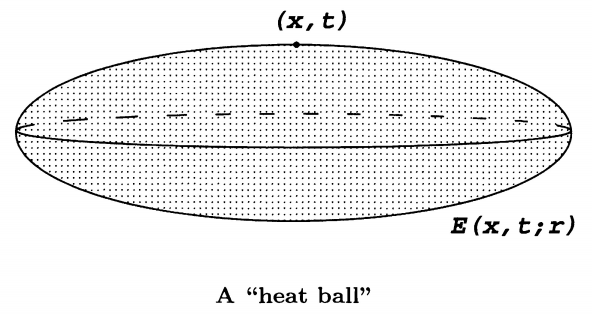
\includegraphics[width=0.52\textwidth]{heat ball.png}
\end{figure}
\begin{remark}
Let us gain some idea of what $E(x,t;r)$ looks like. This is a region in space-time, the boundary of which is a level set of $\Phi(x-y,t-s)$. Note that the point $(x,t)$ is at the center of the top.
Specifically, It is defined by\[\frac{1}{(4\pi(t-s))^{n/2}}\e^{-\frac{|x-y|^2}{4(t-s)}}\geq \frac{1}{r^n}.\]Thus in the time direction, we have $t\geq s\geq t-\frac{r^2}{4\pi}$, where the lower bound comes from the fact that $\e^{-\frac{|x-y|^2}{4(t-s)}}\leq1$. Furthermore
\[E(x,t;r)\cap\{s=0\}=E(x,t;r)\cap\{s=t\}=\{x\}.\]Next, to find out the correct formula, we need to find a kernel $K(x-y,t-s)$ such that\[\iint_{E(x,t;r)}K(x-y,t-s)\dif y\dif s\]is independent of $r$. Notice that
\[\frac{1}{(4\pi(t-s))^{n/2}}\e^{-\frac{|x-y|^2}{4(t-s)}}\geq\frac{1}{r^n} \iff\frac{1}{(4\pi(t^\prime-s^\prime))^{n/2}}\e^{-\frac{|x^\prime-y^\prime|^2}{4(t^\prime-s^\prime)}}\geq1,\]where $t^\prime=t/r^2,s^\prime=s/r^2,x^\prime=x/r,y^\prime=y/r$. Thus we have
\[\int_{E(x,t;r)}K(x-y,t-s)\dif y\dif s=\int_{E(x^\prime,t^\prime;1)}K(x-y,t-s)r^{n+2}\dif y^\prime\dif s^\prime.\]
This implies\[K(x^\prime,t^\prime)=K(x,t)r^{n+2}\]when $x^\prime=x/r,t^\prime=t/r^2$. Now note that\[E(0,0;1)\equiv\left\{\frac{1}{(4\pi t)^{n/2}}\e^{\frac{|x|^2}{4t}}\geq 1\right\}=\left\{0\leq t\leq\frac{1}{4\pi};|x|^2\leq(2nt)\log\frac{1}{4\pi t}\right\},\]and the integral over $E(0,0;1)$ becomes\[\int_0^{1/4\pi}t^{-2} \left[\int_{|x|^2\leq2nt\ln\frac{1}{4\pi t}}|x|^2\dif x\right]\dif t=\frac{n\pi^{n/2}}{n+2} \frac{2^{(n+2)/2}n^{(n+2)/2}}{\Gamma\left(\frac{n}{2}+1\right)}\int_0^{\frac{1}{4\pi}}t^{\frac{n-2}{n}}\left(\ln\frac{1}{4\pi t}\right)^{\frac{n}{2}+1}\dif t.\]Here we have used polar coordinates and the formula $\alpha(n)=\frac{\pi^{n/2}}{\Gamma\left(\frac{n}{2}+1\right)}$ for the volume of $n$-dimension balls. Now setting $s=4\pi t$ and using the formulas\[\lambda^{-z}\Gamma(z)
=\int_0^1t^{\lambda-1}\left(\ln\frac{1}{t}\right)^{z-1}\dif t,\Gamma(z+1)=z\Gamma(z)\] we will see after careful calculations that most terms cancel out and what remains is 4, i.e.
\[\int_{E(0,0 ;1)}\frac{|x|^2}{t^2}\dif x\dif t=4.\]This is exactly what we need.
\end{remark}
\begin{remark}
Since we have mentioned $E(0,0;1)$, we can draw exactly what it looks like when $n=1$. Now\[
\begin{aligned}
	E(0,0;1)&=\left\{(y,s)\in\mr^2:s\leq0,\frac{1}{(4\pi(-s))^{1/2}}\exp \left(-\frac{|-y|^2}{4(-s)}\right)\geq1\right\} \\
	&=\left\{(y,s)\in\mr^2:0<-s\leq\frac{1}{4\pi},y^2\leq2s\ln(-4\pi s)\right\}.
\end{aligned}\]To get $-s\leq\frac{1}{4\pi}$ one simply observe that $\exp\left(-\frac{|-y|^2}{4(-s)}\right)\leq1(s<0)$, and thus $\sqrt{-4\pi s}\leq1$. Hence the boundary of the heat ball is like this:
\begin{figure}[h]
	\centering
	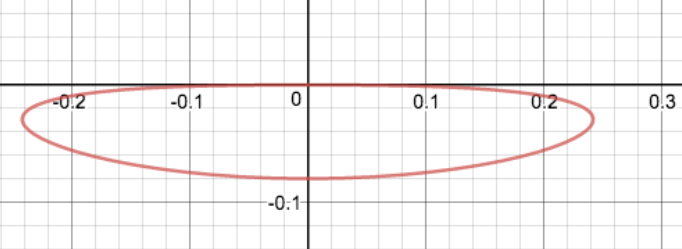
\includegraphics[width=0.58\textwidth]{E(0,0;1).png}
\end{figure}
\end{remark}
\begin{theorem}\label{thm2.205}
(A mean-value property for the heat equation). Let $u\in C_1^2(U_T)$ solve the heat equation. Then\[u(x,t)=\frac{1}{4r^n}\iint_{E(x,t;r)}u(y,s)\frac{|x-y|^2}{(t-s)^2}\dif y\dif s\]for each $E(x,t;r)\subset U_T$.
\end{theorem}
\begin{proof}
See pp53-54 of the book. There is a similar proof of Problem \ref{prob2.17}.
\end{proof}
\begin{remark}
The right-hand side involves only $u(y,s)$ for times $s\leq t$. This is reasonable, as the value $u(x,t)$ should not depend upon future times.
\end{remark}

\noindent\textcolor{blue}{Strong maximum principle, uniqueness.}
\begin{theorem}\label{thm2.20}
(Strong maximum principle for the heat equation). Suppose $u\in C_1^2(U_T)\cap C(\bar{U}_T)$ solves the heat equation in $U_T$.\\
\textup{(i)} Then\[\max_{\bar{U}_T}u=\max_{\Gamma_T}u.\]
\textup{(ii)} Furthermore, if $U$ is connected and there exists a point $(x_0,t_0)\in U_T$ such that\[u(x_0,t_0)=\max_{\bar{U}_T}u,\]
then $u$ is constant in $\bar{U}_{t_0}$.
\end{theorem}
\begin{remark}
Assertion (i) is the maximum principle for the heat equation and (ii) is the strong maximum principle. Similar assertions are valid with "min" replacing "max". If $u$ attains its maximum (or minimum) at an interior point, then $u$ is constant at all earlier times. This means, the solution will be constant on the time interval $[0,t_0]$ provided the initial and boundary conditions are constant. However, the solution may change at times $t>t_0$, provided the boundary conditions alter after $t_0$.
\end{remark}
\begin{proof}
Suppose there exists a point $(x_0,t_0)\in U_T$ with $u(x_0,t_0)=M:=\max\limits_{\bar{U}_T}u$. Then for all sufficiently small $r>0,E(x_0, t_0;r)\subset U_T$; and we employ the mean-value property to deduce
\[M=u(x_0,t_0)=\frac{1}{4r^n}\iint_{E(x_0,t_0;r)}u(y,s)\frac{|x_0-y|^2}{(t_0-s)^2}\dif y\dif s\leq M,\]since\[1=\frac{1}{4r^n}\iint_{E(x_0,t_0;r)}\frac{|x_0-y|^2}{(t_0-s)^2}\dif y\dif s.\]Equality holds only if $u\equiv M$ within $E(x_0,t_0;r)$. Consequently $u(y,s)=M$ for all $(y,s)\in E(x_0,t_0;r)$.

Draw any line segment $L$ in $U_T$ connecting $(x_0,t_0)$ with some other point $(y_0, s_0)\in U_T$, with $s_0<t_0$. Consider\[r_0:=\min\{s\geq s_0:u(x,t)=
M \text{ for all points }(x, t)\in L,s\leq t\leq t_0\}.\]Since $u$ is continuous, the minimum is attained. For the sake of contradiction assume $r_0>s_0$. Then $u(z_0,r_0)=M$ for some point $(z_0,r_0)$ on $L\cap U_T$ and so $u(y,s)\equiv M$ on $E(z_0,r_0;r)$ for all sufficiently small $r>0$. Since $E(z_0,r_0;r)$ contains some point $(x,t)$ with $r_0-\sigma\leq t<r_0$ for some small $\sigma>0$, we have a contradiction. Thus $r_0=s_0$, and hence $u\equiv M$ on $L$.

Now fix any $x\in U$ and $0\leq t<t_0$. There exist points $\{x_0,x_1,\cdots,x_m=x\}$ such that the line segments in $\mr^n$ connecting $x_{i-1}$ to $x_i$ lie in $U$ for $i=1, \cdots,m$. (This follows since  $U$ is connected.) Select times $t_0>t_1>\cdots>t_m=t$. Then the line segments in $\mr^{n+1}$ connecting $(x_{i-1},t_{i-1})$ to $(x_i,t_i)(i=1,\cdots, m)$ lie in $U_T$. According to the previous step, $u\equiv M$ on each such segment and so $u(x,t)=M$.
\end{proof}

An important application of the maximum principle is the following uniqueness assertion.
\begin{theorem}\label{thm2.21}
(Uniqueness on bounded domains). Let $g\in C(\Gamma_T),f \in C(U_T)$. Then there exists at most one solution $u \in C_1^2(U_T)\cap C(\bar{U}_T)$ of the initial/boundary-value problem\[\tag{39}\label{39}\begin{cases}
	\hfill u_t-\Delta u=f&\text{ in } U_T\\
	\hfill u=g&\text{ on } \Gamma_T.
\end{cases}\]
\end{theorem}
\begin{proof}
If $u$ and $\tilde{u}$ are two solutions of (\ref{39}), apply Theorem \ref{thm2.20} to $w:=\pm(u-\tilde{u})$.
\end{proof}

We next extend our uniqueness assertion to the Cauchy problem -- the initial-value problem for $U=\mr^n$. As the region is no longer bounded, we must introduce some control on the behavior of solutions for large $|x|$.
\begin{theorem}\label{thm2.22}
(Maximum principle for the Cauchy problem). Suppose $u\in C_1^2(\mr^n\times(0,T])\cap C(\mr^n\times[0,T])$ solves\[\left\{\begin{aligned}
	u_t-\Delta u=0&\quad\text{ in } \mr^n\times(0,T)\\
	u=g&\quad\text{ on }\mr^n\times\{t=0\}
\end{aligned}\right.\]
and satisfies the growth estimate\[u(x,t)\leq A\e^{a|x|^2}(x\in\mr^n,0\leq t\leq T)\]
for constants $A, a>0$. Then\[\sup_{\mr^n\times[0,T]}u=\sup_{\mr^n}g.\]
\end{theorem}
\begin{proof}
First assume $4aT<1$ in which case $4a(T+\ve)<1$ for some $\ve>0$. Fix $y\in\mr^n,\mu> 0$, and define\[v(x,t):=u(x,t)-\frac{\mu}{(T+\ve-t)^{n/2}}\e^{\frac{|x-y|^2} {4(T+\ve-t)}}(x\in\mr^n,t>0).\]A direct calculation shows
\[v_t-\Delta v=0\quad\text{ in } \mr^n\times(0,T].\]Fix $r>0$ and set $U:=B^0(y,r)$, and then $U_T=B^0(y,r)\times(0,T]$. Then according to Theorem \ref{thm2.20},\[\tag{40}
\max_{\bar{U}_T}v=\max_{\Gamma_T}v.\label{40}\]

For $x\in\mr^n$,\[\tag{41}v(x,0)=u(x,0)-\frac{\mu}{(T+\ve)^{n/2}}\e^{\frac{|x-y|^2} {4(T+\ve)}}\leq u(x,0)=g(x);\label{41}\]and if $|x-y|=r, 0 \leq t \leq T$, then
\[\begin{aligned}
	v(x,t)=u(x,t)-\frac{\mu}{(T+\ve-t)^{n/2}}\e^{\frac{r^2}{4(T+\ve-t)}}&\leq A\e^{a|x|^2}-\frac{\mu}{(T+\ve-t)^{n/2}}\e^{\frac{r^2}{4(T+\ve-t)}}\\
	&\leq A\e^{a(|y|+r)^2}-\frac{\mu}{(T+\ve)^{n/2}}\e^{\frac{r^2}{4(T+\ve)}}.
\end{aligned}\]Because $4a(T+\ve)<1$, we have $\frac{1}{4(T+\ve)}>a$, and so $\frac{1}{4(T+\ve)}=a+\gamma$ for some $\gamma>0$. Then we continue to find\[v(x,t)
\leq A\e^{a(|y|+r)^2}-\mu(4(a+\gamma))^{n/2}\e^{(a+\gamma)r^2}\leq\sup_{\mr^n}g,\] for $r$ selected sufficiently large. Thus this combined with (\ref{40}) and (\ref{41}), imply that $v(y,t)\leq\sup\limits_{\mr^n}g$ for all $y\in\mr^n,0\leq t\leq T$. Now let $\mu\to0$.

In the general case that $4aT<1$ fails, we repeatedly apply the result above on the time intervals $[0,T_1],[T_1,2T_1]$, etc., for $T_1=\frac{1}{8a}$.
\end{proof}
\begin{theorem}\label{thm2.23}
(Uniqueness for Cauchy problem). Let $g\in C(\mr^n),f\in C(\mr^n\times[0,T])$. Then there exists at most one solution $u\in C_1^2(\mr^n\times(0,T])\cap C(\mr^n\times[0,T])$ of the initial-value problem\[\left\{\begin{aligned}
	u_t-\Delta u=0&\quad\text{ in } \mr^n\times(0,T)\\
	u=g&\quad\text{ on }\mr^n\times\{t=0\}
\end{aligned}\right.\]satisfying the growth estimate\[u(x,t)\leq A\e^{a|x|^2}(x\in\mr^n,0\leq t\leq T)\]for constants $A,a>0$.
\end{theorem}
\begin{proof}
If $u$ and $\tilde{u}$ both satisfy the conditions, we apply Theorem \ref{thm2.22} to $w:=\pm(u-\tilde{u})$ to know that $w\equiv0$ in $\mr^n\times(0,T)$.
\end{proof}

\noindent\textcolor{blue}{Regularity.}
\begin{theorem}\label{thm2.25}
(Smoothness). Suppose $u\in C_1^2(U_T)$ solves the heat equation in $U_T$. Then\[u\in C^\infty(U_T).\]
\end{theorem}
\begin{proof}
Define $C(x,t;r)=\{(y,s):|x-y|\leq r,t-r^2\leq s\leq t\}$ to be the closed circular cylinder of radius $r$, height $r^2$, and top center point $(x,t)$.

Fix $(x_0,t_0)\in U_T$ and choose $r>0$ so small that $C:=C(x_0,t_0;r)\subset U_T$. Define also the smaller cylinders $C^\prime:=C(x_0,t_0;\frac{3}{4}r),C^{\prime\prime}:= C(x_0,t_0;\frac{1}{2}r)$, which have the same top center point $(x_0,t_0)$.

Now we set a smooth cutoff function $\zeta=\zeta(x,t)$ such that\[\left\{\begin{array}{l}
	0\leq\zeta\leq1,\zeta\equiv1\quad\text{on } C^\prime\\
	\zeta\equiv0\quad\text{ near the parabolic boundary of } C.
\end{array}\right.\]Extend $\zeta\equiv0$ in $(\mr^n\times[0,t_0])-C$.
\begin{figure}[h]
	\centering
	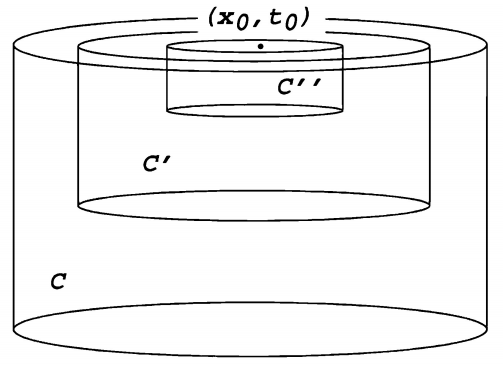
\includegraphics[width=0.5\textwidth]{cylinder.png}
\end{figure}

Assume temporarily that $u\in C^\infty(U_T)$ and set
\[v(x,t):=\zeta(x,t)u(x,t)(x\in\mr^n,0\leq t\leq t_0).\]Then
\[v_t=\zeta u_t+\zeta_tu,\Delta v=\zeta\Delta u+2D\zeta\cdot Du+u\Delta\zeta.\]
Consequently $v_t-\Delta v=\zeta_t u-2D\zeta\cdot Du-u\Delta\zeta=:\tilde{f}$ in $\mr^n \times(0,t_0)$ and $v=0$ on $\mr^n\times\{t=0\}$. Now set \[\tilde{v}(x,t):=\int_0^t\int_{\mr^n}\Phi(x-y,t-s)\tilde{f}(y,s)\dif y\dif s,\]and according to Theorem \ref{thm2.18}, $\tilde{v}$ solves \[\left\{\begin{aligned}
	\tilde{v}_t-\Delta\tilde{v}=\tilde{f}&\quad\text{ in } \mr^n\times(0,t_0)\\
	\tilde{v}=0&\quad\text{ on } \mr^n \times\{t=0\}.
\end{aligned}\right.\]Since $|v|,|\tilde{v}|\leq A$ for some constant $A$, Theorem \ref{thm2.23} implies that $v\equiv\tilde{v}$; that is, \[v(x,t)=\int_0^t\int_{\mr^n}\Phi(x-y,t-s)\tilde{f}(y,s)\dif y\dif s.\]
Now suppose $(x,t)\in C^{\prime\prime}$. As $\zeta\equiv0$ off $C$, then we have \[\tag{42}\label{42}\begin{aligned}
	&u(x,t)=\iint_C\Phi(x-y,t-s)\tilde{f}(y,s)\dif y\dif s=\iint_C\Phi(x-y,t-s)(v_s-\Delta v)\dif y\dif s\\
	=&\iint_C\Phi(x-y,t-s)[u(y,s)(\zeta_s(y,s)-\Delta\zeta(y,s))-2D\zeta(y,s)\cdot Du(y,s)]\dif y\dif s.
\end{aligned}\]Note in the equation that \[\begin{aligned}
&\iint_CD_y(D\zeta(y,s)\Phi(x-y,t-s)u(y,s))\dif y\dif s\\
=&\int_0^t\dif s\int_{B(x_0,r)}D_y(D_y\zeta(y,s)\Phi(x-y,t-s)u(y,s))\dif y\\
=&\int_0^t\dif s\int_{\ptl B(x_0,r)}\Phi(x-y,t-s)u(y,s)\mathop{(D\zeta(y,s))}_{=0~ \text{on}~\ptl C}\cdot\bm{\nu}\dif S(y)=0.
\end{aligned}\]This implies, using integration by parts, \[\tag{43}\label{43}\begin{aligned}
0=2\bigg[\iint_C\Delta\zeta(y,s)\Phi(x-y,t-s)u(y,s)+&D\zeta(y,s)D_y\Phi(x-y,t-s)u(y,s)\\
&+D\zeta(y,s)\Phi(x-y,t-s)Du(y,s)\dif y\dif s\bigg].
\end{aligned}\]Adding (\ref{43}) to (\ref{42}), we obtain\[\tag{44}\label{44}\begin{aligned}
u(x,t)=\iint_Cu(y,s)\big[&\Phi(x-y, t-s)(\zeta_s(y,s)-\Delta\zeta(y,s))\\
&+2D_y\Phi(x-y,t-s)\cdot D\zeta(y,s)\big]\dif y\dif s.
\end{aligned}\]We have proved this formula assuming $u\in C^\infty$. If $u$ satisfies only the hypotheses of the theorem, we derive (\ref{44}) with $u^\ve=\eta_\ve*u$ replacing $u,\eta_\ve$ being the standard mollifier in the variables $x$ and $t$, and let $\ve\to0$.

Formula (\ref{44}) has the form
\[u(x,t)=\iint_CK(x,t,y,s)u(y,s)\dif y\dif s((x,t)\in C^{\prime\prime}),\]where $K(x,t,y,s)= 0$ for all $(y,s)\in C^\prime$ since $\zeta\equiv1$ on $C^\prime$. Note also $K$ is smooth on $C-C^\prime$. Now we see $u$ is $C^\infty$ within $C^{\prime\prime}$.
\end{proof}
\begin{remark}
This regularity assertion is valid even if $u$ attains nonsmooth boundary values on $\Gamma_T$.
\end{remark}

\noindent\textcolor{blue}{Energy methods.} We investigate again the initial/boundary-value problem (\ref{39}). We have seen uniqueness in Theorem \ref{thm2.21}, but now, by analogy, with Laplace's equation, we provide an alternative argument. Assume as usual $U\in\mr^n$ is open and bounded, and $\ptl U$ is $C^1$. $T>0$ is given.
\begin{theorem}
(Uniqueness). There exists only one solution $u\in C_1^2(\bar{U}_T)$ of (\ref{39}).
\end{theorem}
\begin{proof}
If $\tilde{u}$ is another solution, then $w:=u-\tilde{u}$ solves\[\left\{\begin{aligned}
	w_t-\Delta w=0&\quad\text{ in } U_T \\
	w=0&\quad\text{ on } \Gamma_T .
\end{aligned}\right.\]Set $e(t):=\dis\int_Uw^2(x,t)\dif x(0\leq t\leq T)$, and so
\[\begin{aligned}
	e^\prime(t)&=2\int_Uww_t\dif x=2\int_Uw\Delta w\dif x=2\left[-\int_UDw\cdot Dw\dif x+\int_Uw\frac{\ptl w}{\ptl\nu}\dif S\right]\\
	&=-2\int_U|Dw|^2\dif x\leq0.
\end{aligned}\]Hence $e(t)\leq e(0)=0$, showing that $w=u-\tilde{u}\equiv0$ in $U_T$.
\end{proof}
\begin{remark}
Compare this theorem with Theorem \ref{thm2.15}.
\end{remark}

A more subtle question asks about uniqueness backwards in time. Suppose $u$ and $\tilde{u}$ are both smooth solutions of the heat equation in $U_T$, with the same boundary conditions on $\ptl U$:\[\tag{45}\label{45}\left\{\begin{aligned}
	u_t-\Delta u=0&\quad\text{ in } U_T\\
	u=g&\quad\text{ on } \ptl U \times[0,T],
\end{aligned}\right.\]\[\tag{46}\label{46}\left\{\begin{aligned}
\tilde{u}_t-\Delta\tilde{u}=0&\quad\text{ in } U_T\\
\tilde{u}=g&\quad\text{ on } \ptl U \times[0,T].
\end{aligned}\right.\]Note that we do NOT suppose $u=\tilde{u}$ at time $t=0$.
\begin{theorem}
(Backwards uniqueness). Suppose $u,\tilde{u}\in C^2(\bar{U}_T)$ solve (\ref{45}), (\ref{46}). If\[u(x,T)=\tilde{u}(x,T)(x\in U),\] then $u\equiv\tilde{u}$ within $U_T$.
\end{theorem}
\begin{proof}
Again write $w:=u-\tilde{u}$ and set\[e(t):=\int_Uw^2(x,t)\dif x(0\leq t\leq T).\]As before \[e^\prime(t)=-2\int_U|Dw|^2\dif x,\]and\[\begin{aligned}
	e^{\prime\prime}(t)&=-4\int_UDw\cdot Dw_t\dif x=-4\left[-\int_Uw_t\Delta w\dif x+\int_{\ptl U}w_t\frac{\ptl w}{\ptl\nu}\dif S\right]\\
	&=4\int_U\Delta w\cdot w_t\dif x=4\int_U(\Delta w)^2\dif x
\end{aligned}\]since $w_t-\Delta w=0$ in $U_T$. Now because $w=0$ on $\ptl U$, we employ Cauchy-Schwarz inequality:\[\int_U|Dw|^2\dif x=-\int_Uw\Delta w\dif x
\leq\left(\int_Uw^2\dif x\right)^{1/2}\left(\int_U(\Delta w)^2\dif x\right)^{1/2}.\]Thus \[(e^\prime(t))^2=4\left(\int_U|Dw|^2\dif x\right)^2\leq e(t)e^{\prime\prime}(t),\]i.e. $e(t)e^{\prime\prime}(t)\geq(e^\prime(t))^2(0\leq t\leq T)$.

Now if $e(t)=0$ for all $0\leq t\leq T$, we are done. Otherwise there exists an interval $[t_1,t_2]\subset[0,T]$, with $e(t)>0$ for $t_1\leq t<t_2$, and $e(t_2)=0$. Write $f(t):=\ln e(t)(t_1\leq t<t_2)$. Then\[f^{\prime\prime}(t)=\frac{e^{\prime\prime}(t)}
{e(t)}-\frac{e^\prime(t)^2}{e(t)^2}\geq0,\]and so $f$ is convex on the interval $(t_1,t_2)$. Consequently if $0<\tau<1$, $t_1<t<t_2$, we have
\[f((1-\tau)t_1+\tau t)\leq(1-\tau)f(t_1)+\tau f(t).\]Hence $\ln e((1-\tau)t_1+\tau t)\leq (1-\tau)\ln e(t_1)+\tau\ln e(t_2)$, which further reduces to\[e((1-\tau)t_1+\tau t)\leq e^{1-\tau}(t_1)e^\tau(t).\]But\[0\leq e((1-\tau)t_1+\tau t_2)\leq e(t_1)^{1-\tau} e(t_2)^\tau=0(0<\tau<1),\]contradicting the claim that $e(t)>0$ for $t_1\leq t<t_2$.
\end{proof}
\begin{remark}
In other words, if two temperature distributions on $U$ agree at some time $T>0$ and have had the same boundary values for times $0\leq t\leq T$, then these temperatures must have been identically equal within $U$ at all earlier times.
\end{remark}

\subsection{Wave equation}
In this section we investigate the wave equation{\color{red}\[u_{tt}-\Delta u=0\tag{47}\label{wave1}\]}and the nonhomogeneous wave equation{\color{red}\[u_{tt}-\Delta u=f,\tag{48}\label{wave2}\]}subject to appropriate initial and boundary conditions. Here $t>0$ and $x\in U$, where $U\subset\mr^n$ is open. The unknown is $u=u(x,t):\bar{U}\times[0,\infty)\to\mr$. In (\ref{wave2}) the function $f: U\times[0,\infty)\to\mr$ is given.
\begin{remark}
We shall discover that solutions of the wave equation behave quite differently than solutions of Laplace's equation or the heat equation. Please always pay attention to the difference between them.
\end{remark}

\noindent\textcolor{blue}{Solution for $n=1$, d'Alembert's formula.} We first focus our attention on the initial-value problem for the one-dimensional wave equation in all of $\mr$:
\[\tag{49}\label{49}\left\{\begin{array}{cl}
	u_{tt}-u_{xx}=0 & \text{ in } \mr\times(0,\infty)\\
	u=g,u_t=h & \text{ on } \mr\times\{t=0\},
\end{array}\right.\]where $g,h$ are given. We desire to derive a formula for $u$ in terms of $g$ and $h$.

Let us first note that the PDE in (\ref{49}) can be "factored", to read
\[\left(\frac{\ptl}{\ptl t}+\frac{\ptl}{\ptl x}\right)\left(\frac{\ptl}{\ptl t}-\frac{\ptl}{\ptl x}\right)u=u_{tt}-u_{xx}=0.\]Write $v(x,t):=\dis\left(\frac{\ptl}{\ptl t}-\frac{\ptl}{\ptl x}\right)u(x,t)$, and then $v_t(x,t)+v_x(x,t)=0(x\in\mr,t>0)$. This is a transport equation with constant coefficients. Applying the formula for the homogeneous transport equation (with $n=1,b=1$), we find $v(x,t)=a(x-t)$ for for $a(x):=v(x,0)$. Now we have \[u_t(x,t)-u_x(x,t)
=a(x-t)\quad\text{ in } \mr\times(0,\infty).\]This is a nonhomogeneous transport equation; so the formula $u(x,t)=g(x-tb)+\dis\int_0^tf(x+(s-t)b,s)\dif s$ (with $n=1,b=-1,f(x,t)=a(x-t)$) implies for $b(x):=u(x,0)$ that\[u(x,t)=\int_0^ta(x+(t-s)-s)\dif s+
b(x+t)\xlongequal{x+t-2s=y}\frac{1}{2}\int_{x-t}^{x+t}a(y)\dif y+b(x+t).\]We lastly invoke the initial conditions of (\ref{49}) to compute $a$ and $b$. The first condition gives $b(x)=g(x)$, while the second implies $a(x)=v(x,0)=u_t(x,0)-u_x(x,0)=h(x)-g^\prime(x)$. Our substitution now yields\[u(x,t)=\frac{1}{2}\int_{x-t}^{x+t}(h(y)-g^\prime(y))\dif y+g(x+t).\]Hence\[u(x,t)=\frac{1}{2}[g(x+t)+g(x-t)]+\frac{1}{2}\int_{x-t}^{x+t}h(y)\dif y(x\in \mr,t\geq0).\tag{50}\label{50}\]This is \emph{d'Alembert's formula}.
\begin{theorem}
(Solution of wave equation, $n=1$). Assume $g\in C^2(\mr),h\in C^1(\mr)$, and define $u$ by d'Alembert's formula \textup{(\ref{50})}. Then\\
\textup{(i)} $u\in C^2(\mr\times[0,\infty))$,\\
\textup{(ii)} $u_{tt}-u_{xx}=0$ in $\mr\times(0,\infty)$,\\
and\\
\textup{(iii)} $\limls_{\substack{(x,t)\to(x^0,0)\\t>0}}u(x,t)=g(x^0),\limls_{\substack{(x,t)\to(x^0,0)\\t>0}}u_t(x,t)=h(x^0)$ for each point $x^0\in\mr$.
\end{theorem}
\begin{proof}
This is a straightforward calculation.
\end{proof}
\begin{remark}
(i) Our solution $u$ has the form $u(x,t)=F(x+t)+G(x-t)$ for appropriate $F$ and $G$. Conversely any function of this form solves $u_{tt}-u_{xx}=0$. Hence the general solution of the one-dimensional wave equation is a sum of the general solution of $u_t-u_x=0$ and that of $u_t+u_x=0$. This is a consequence of the factorization.

(ii) if $g\in C^k$ and $h\in C^{k-1}$, then $u\in C^k$ but is not in general smoother.
\end{remark}

\noindent\textcolor{blue}{A reflection method.} To illustrate an application of d'Alembert's formula, let us next consider this initial/boundary-value problem on $\mr_+=\{x>0\}$: \[\tag{51}\label{51}\left\{\begin{aligned}
	u_{tt}-u_{xx}=0&\quad\text{ in } \mr_+\times(0,\infty)\\
	u=g,u_t=h&\quad\text{ on } \mr_+\times\{t=0\}\\
	u=0&\quad\text{ on }\{x=0\}\times(0,\infty),
\end{aligned}\right.\]where $g,h$ are given, with $g(0)=h(0)=0$.

We convert (\ref{51}) into the form (\ref{49}) by extending $u,g,h$ to all of $\mr$ by odd reflection. That is, we set\[\begin{aligned}
	\tilde{u}(x,t)&:=\begin{cases}u(x,t)&(x\geq0,t\geq0) \\
		-u(-x,t)&(x\leq0,t\geq0),\end{cases}\\
	\tilde{g}(x)&:=\begin{cases}g(x)&(x\geq0)\\
		-g(-x)&(x\leq0),\end{cases}\\
	\tilde{h}(x)&:=\begin{cases}h(x)&(x\geq0)\\
		-h(-x)&(x\leq0).\end{cases}
\end{aligned}\]Then (\ref{51}) becomes \[\begin{cases}\tilde{u}_{tt}=\tilde{u}_{xx}& \text{ in } \mr\times(0,\infty)\\ \tilde{u}=\tilde{g},\tilde{u}_t=\tilde{h}& \text{ on } \mr\times\{t=0\}.\end{cases}\]Hence d'Alembert's formula (\ref{50}) implies
\[\tilde{u}(x,t)=\frac{1}{2}[\tilde{g}(x+t)+\tilde{g}(x-t)]+\frac{1}{2}\int_{x-t}^{x+t} \tilde{h}(y)\dif y.\]Then \[\tag{52}\label{52}
u(x,t)=\begin{cases}\frac{1}{2}[g(x+t)+g(x-t)]+\frac{1}{2}\int_{x-t}^{x+t}h(y)\dif y & \text{ if } x\geq t\geq0\\ \frac{1}{2}[g(x+t)-g(t-x)]+\frac{1}{2}\int_{-x+t}^{x+t} h(y)\dif y&\text{ if } 0\leq x\leq t.\end{cases}\]

\noindent\textcolor{blue}{Spherical means.} Now suppose $n\geq2,m\geq2$, and $u\in C^m(\mr^n\times[0,\infty))$ solves the initial-value problem\[\tag{53}\begin{cases}
u_{tt}-\Delta u=0& \text { in } \mr^n\times(0,\infty)\\u=g,u_t=h& \text{ on } \mr^n \times\{t=0\}.\end{cases}\label{53}\]Let $x\in\mr^n,t>0,r>0$. Define
\[U(x;r,t):=\dashint_{\ptl B(x,r)}u(y,t)\dif S(y),\]the average of $u(\cdot,t)$ over the sphere $\ptl B(x,r)$. Similarly, \[G(x;r):=\dashint_{\ptl B(x,r)}g(y)\dif S(y),H(x;r):= \dashint_{\ptl B(x,r)}h(y)\dif S(y).\]For fixed $x$, we hereafter regard $U$ as a function of $r$ and $t$.
\begin{lemma}\label{EPD}
(Euler-Poisson-Darboux equation). Fix $x\in\mr^n$, and let $u$ satisfy \textup{(\ref{53})}. Then $U\in C^m(\overline{\mr}_+\times[0,\infty))$ and \[\left\{\begin{aligned}
	U_{tt}-U_{rr}-\frac{n-1}{r}U_r=0 &\quad\text{ in } \mr_+\times(0,\infty)\\
	U=G,U_t=H&\quad\text{ on } \mr_+\times\{t=0\}.
\end{aligned}\right.\]
\end{lemma}
\begin{remark}
The term $U_{rr}+\frac{n-1}{r}U_r$ is the radial part of the Laplacian $\Delta$ in polar coordinates.
\end{remark}
\begin{proof}
As in the proof of Theorem \ref{MVF1} we compute for $r>0$ \[U_r(x;r,t)=\frac{r}{n}
\dashint_{B(x,r)}\Delta u(y,t)\dif y.\tag{54}\label{54}\]From this we deduce $\limls_ {r\to0^+}U_r(x;r,t)=0$. Next we differentiate (\ref{54}) to discover that\[\begin{aligned}
	U_{rr}(x;r,t)&=\frac{\ptl}{\ptl r}\left(\frac{r}{n}\frac{1}{\alpha(n)r^n}\int_{B(x,r)} \Delta u(y,t)\dif y\right)\\
	&=\frac{1}{n\alpha(n)}\left[(1-n)r^{-n}\int_{B(x,r)}\Delta u(y,t)\dif y+\frac{1}{r^{n-1}}\frac{\ptl}{\ptl r}\int_{B(x,r)}\Delta u\dif y\right]\\
	&=\frac{1-n}{n\alpha(n)r^n}\int_{B(x,r)}\Delta u\dif y+\frac{1}{n\alpha(n)r^{n-1}} \frac{\ptl}{\ptl r}\int_0^r\dif s\int_{\ptl B(x,s)}\Delta u\dif S(y)\\
	&=\left(\frac{1}{n}-1\right)\dashint_{B(x,r)}\Delta u\dif y+\dashint_{\ptl B(x,r)}\Delta u\dif S.
\end{aligned}\]Thus $\limls_{r\to0^+}U_{rr}(x;r,t)=\dfrac{1}{n}\Delta u(x,t)$. We can continue computing $U_{rrr}$, etc., and so verify that $U\in C^m(\overline{\mr}_+\times[0,\infty))$.

Continuing the calculation above, we see from (\ref{54}) that\[\begin{aligned}
	U_r&=\frac{r}{n}\dashint_{B(x,r)}u_{tt}\dif y\quad\text{ by (\ref{53})}\\
	& =\frac{1}{n\alpha(n)}\frac{1}{r^{n-1}}\int_{B(x,r)}u_{tt}\dif y.
\end{aligned}\]And so \[
(r^{n-1}U_r)_r=\frac{1}{n\alpha(n)}\int_{\ptl B(x,r)}u_{tt}\dif S=r^{n-1}\dashint_{\ptl B(x,r)}u_{tt}\dif S=r^{n-1}U_{tt}.\]It follows immediately that $U_{tt}-U_{rr}-\frac{n-1}{r}U_r=0$.
\end{proof}

\noindent\textcolor{blue}{Solution for $n=3$, Kirchhoff's formula.} Let us take $n=3$, and suppose $u\in C^2(\mr^3\times[0,\infty))$ solves (\ref{53}). Recall the definitions of $U,G,H$ and then set \[\tilde{U}:=rU,\tilde{G}:=rG,\tilde{H}:=rH.\]We now assert that $\tilde{U}$ solves\[\left\{\begin{aligned}
	\tilde{U}_{tt}-\tilde{U}_{rr}&=0&& \text{ in } \mr_+\times(0,\infty)\\
	\tilde{U}=\tilde{G},\tilde{U}_t&=\tilde{H}& & \text{ on } \mr_+\times\{t=0\} \\
	\tilde{U}&=0&& \text{ on }\{r=0\}\times(0,\infty).
\end{aligned}\right.\tag{55}\label{55}\]Indeed, by\[\begin{aligned}
\tilde{U}_{tt}&=rU_{tt}=r\left[U_{rr}+\frac{2}{r}U_r\right] \quad \text { by Lemma } \ref{EPD},\text{ with } n=3\\
&=rU_{rr}+2U_r=(U+rU_r)_r=\tilde{U}_{rr}.
\end{aligned}\]Notice also that $\tilde{G}_{rr}(0)=0$. Applying formula (\ref{52}) to (\ref{55}), we find for $0\leq r\leq t$ \[\tilde{U}(x;r,t)=\frac{1}{2}[\tilde{G}(r+t)- \tilde{G}(t-r)]+\frac{1}{2}\int_{-r+t}^{r+t}\tilde{H}(y)\dif y.\]Since $\limls_{r\to0^+}U(x;r,t)=u(x,t)$, we conclude that\[\begin{aligned}
u(x,t)&=\lim_{r\to0^+}\frac{\tilde{U}(x;r,t)}{r}=\lim_{r\to0^+}\left[\frac{\tilde{G}(t+r)-\tilde{G}(t-r)}{2r}+\frac{1}{2r} \int_{t-r}^{t+r}\tilde{H}(y)\dif y\right]\\
&=\tilde{G}^\prime(t)+\tilde{H}(t).
\end{aligned}\]By definitions of $\tilde{G}$ and $\tilde{H}$ we deduce \[\tag{56}\label{56}u(x,t)=\frac{\ptl}{\ptl t}\left(t\dashint_{\ptl B(x,t)}g\dif S\right)+t\dashint_{\ptl B(x,t)}h\dif S.\]But\[
\dashint_{\ptl B(x,t)}g(y)\dif S(y)=\dashint_{\ptl B(0,1)}g(x+tz)\dif S(z);\]and so\[\frac
{\ptl}{\ptl t}\left(\dashint_{\ptl B(x,t)}g\dif S\right)=\dashint_{\ptl B(0,1)}Dg(x+tz) \cdot z \dif S(z)=\dashint_{\ptl B(x,t)}Dg(y)\cdot\left(\frac{y-x}{t}\right)\dif S(y).\] Therefore we know $\dis\frac{\ptl}{\ptl t}\left(t\dashint_{\ptl B(x,t)}g\dif S\right)$ and hence\[\tag{57}\label{57}u(x,t)=\dashint_{\ptl B(x,t)}th(y)+g(y)+Dg(y)\cdot(y-x)\dif S(y) (x\in\mr^3,t>0).\]This is \emph{Kirchhoff's formula}.

\noindent\textcolor{blue}{Solution for $n=2$, Poisson's formula.} Now no transformation works to convert Euler-Poisson-Darboux equation into the one-dimensional wave equation when $n=2$. Instead we will take (\ref{53}) for $n=2$ and simply regard it as a problem for $n=3$, in which the third spatial variable $x_3$ does not appear. Indeed, assuming $u\in C^2(\mr^2\times[0,\infty))$ solves (\ref{53}) for $n=2$, let us write $\bar{u}(x_1,x_2,x_3,t):=u(x_1,x_2,t)$. Then (\ref{53}) implies\[\left\{\begin{array}{cl}
	\bar{u}_{tt}-\Delta\bar{u}=0& \text { in } \mr^3\times(0,\infty) \\
	\bar{u}=\bar{g},\bar{u}_t=\bar{h}& \text { on } \mr^3 \times\{t=0\},
\end{array}\right.\]for $\bar{g}(x_1,x_2,x_3):=g(x_1,x_2),\bar{h}(x_1,x_2,x_3):=h(x_1,x_2)$. If we write $x=(x_1,x_2)\in\mr^2$ and $\bar{x}=(x_1,x_2,0)\in\mr^3$, then Kirchhoff's formula in the form (\ref{56}) imply\[\tag{58}u(x,t)=\bar{u}(\bar{x},t)=\frac{\ptl}{\ptl t} \left(t\dashint_ {\ptl\bar{B}(\bar{x},t)}\bar{g}\dif \bar{S}\right)+t\dashint_{\ptl \bar{B}(\bar{x},t)}\bar{h}\dif\bar{S},\label{58}\]where $\bar{B}(\bar{x},t)$ denotes the ball in $\mr^3$ with center $\bar{x}$, radius $t>0$ and where $\dif\bar{S}$ denotes two-dimensional surface measure on $\ptl\bar{B}(\bar{x},t)$. Observe that \[\dashint_{\ptl\bar{B}(\bar{x},t)}\bar{g}\dif\bar {S}=\frac{1}{4\pi t^2}\int_ {\ptl\bar{B}(\bar{x},t)}\bar{g}(y)\dif\bar{S}(y)=\frac{2}{4\pi t^2}\int_{B(x,t)}g(y) \sqrt{1+|D\gamma(y)|^2}\dif y,\]where $\gamma(y)=\sqrt{t^2-|y-x|^2}$ for $y\in B(x,t)$. The factor "2" enters since $\ptl\bar{B}(\bar{x},t)$ consists of two hemispheres. Thus $D\gamma(y)=\dfrac{|y-x|} {\sqrt{t^2-|y-x|^2}}$, and $\sqrt{1+|D\gamma(y)|^2}=\left(\dfrac{t^2}{t^2-|y-x|^2}\right) ^{1/2}$, and hence\[\dashint_{\ptl\bar{B}(\bar{x},t)}\bar{g}\dif\bar{S}=\frac{1}{2\pi t}
\int_{B(x,t)} \frac{g(y)}{(t^2-|y-x|^2)^{1/2}}\dif y=\frac{t}{2}\dashint_{B(x,t)}
\frac{g(y)}{(t^2-|y-x|^2)^{1/2}}\dif y.\]Consequently (\ref{58}) becomes\[u(x,t)=
\frac{\ptl}{\ptl t}\left(\frac{t^2}{2}\dashint_{B(x,t)}\frac{g(y)}{(t^2-|y-x|^2)^{1/2}}\dif y\right)+\frac{t^2}{2}\dashint_{B(x,t)}\frac{h(y)}{(t^2-|y-x|^2)^{1/2}}\dif y.\]But\[t^2
\dashint_{B(x,t)}\frac{g(y)}{(t^2-|y-x|^2)^{1/2}}\dif y=t\dashint_{B(0,1)}\frac{g(x+tz)} {(1-|z|^2)^{1/2}}\dif z,\]and so\[\begin{aligned}
	\frac{\ptl}{\ptl t}&\left(t^2\dashint_{B(x, t)}\frac{g(y)}{(t^2-|y-x|^2)^{1/2}}\dif y\right)\\
	&=\dashint_{B(0,1)}\frac{g(x+tz)}{(1-|z|^2)^{1/2}}\dif z+t\dashint_{B(0,1)}\frac{D g(x+tz)\cdot z}{(1-|z|^2)^{1/2}}\dif z\\
	&=t\dashint_{B(x,t)}\frac{g(y)}{(t^2-|y-x|^2)^{1/2}}\dif y+t\dashint_{B(x,t)}\frac{Dg(y)\cdot(y-x)}{(t^2-|y-x|^2)^{1/2}}\dif y.
\end{aligned}\]Hence we obtain the relation\[\tag{59}u(x,t)=\frac{1}{2}\dashint_{B(x,t)}
\frac{tg(y)+t^2h(y)+tDg(y)\cdot(y-x)}{(t^2-|y-x|^2)^{1/2}}\dif y\label{59}\]for $x\in\mr^2,t>0$. This is \emph{Poisson's formula}.
\begin{remark}
The trick of solving the problem for $n=3$ first and then dropping to $n=2$ is the \emph{method of descent}.
\end{remark}

\noindent\textcolor{blue}{Conclusions of cases $n>3$.} In this part, you only need to notice the differentiability of the solution, while the rest is for reference only. First, for odd $n\geq3$, we again solve the Euler-Poisson-Darboux PDE to gain the solution.
\begin{theorem}\label{thm2.28}
(Solution of wave equation in odd dimensions). Assume $n$ is an odd integer, $n \geq 3$, and suppose also $g\in C^{m+1}(\mr^n), h\in C^m(\mr^n)$, for $m=\frac{n+1}{2}$. Define $u$ by \[u(x,t)=\frac{1}{\gamma_n}\left[\frac{\ptl}{\ptl t}\left(\frac{1}{t} \frac{\ptl}{\ptl t}\right)^{\frac{n-3}{2}}\left(t^{n-2}\dashint_{\ptl B(x,t)}g\dif S\right)+\left(\frac{1}{t}\frac{\ptl}{\ptl t}\right)^{\frac{n-3}{2}}\left(t^{n-2}\dashint_{\ptl B(x,t)}h\dif S\right)\right],\]where $n$ is odd, $\gamma_n=1\cdot3\cdot5\cdots(n-2),x\in\mr^n$ and $t>0$. Then\\
\textup{(i)} $u\in C^2(\mr^n\times[0,\infty))$,\\
\textup{(ii)} $u_{tt}-\Delta u=0$ in $\mr^n\times(0,\infty)$,\\and\\ \textup{(iii)}
 $\limls_{\substack{(x,t)\to(x^0,0)\\x\in\mr^n,t>0}}u(x,t)=g(x^0),\limls_{\substack {(x,t)\to(x^0,0)\\x\in\mr^n,t>0}}u_t(x,t)=h(x^0)$ for each point $x^0\in\mr^n$.
\end{theorem}
While for even $n$, we use the method of descent again. Define $u$ by\[\begin{aligned}
	u(x, t)=\frac{1}{\gamma_n}\bigg[&\frac{\ptl}{\ptl t}\left(\frac{1}{t}\frac{\ptl}{\ptl t}\right)^{\frac{n-2}{2}}\left(t^n\dashint_{B(x,t)}\frac{g(y)}{(t^2-|y-x|^2)^{1/2}}\dif y\right)\\
	&\quad+\left(\frac{1}{t}\frac{\ptl}{\ptl t}\right)^{\frac{n-2}{2}}\left(t^n\dashint_{B(x,t)}\frac{h(y)}{(t^2-|y-x|^2)^{1/2}}\dif y\right)\bigg],
\end{aligned}\]where $n$ is even, $\gamma_n=2\cdot4\cdots(n-2)\cdot n,x\in\mr^n$ and $t>0$. Then
\begin{theorem}\label{thm2.29}
(Solution of wave equation in even dimensions). Assume $n$ is an even integer, $n\geq2$, and suppose also $g\in C^{m+1}(\mr^n),h\in C^m(\mr^n)$, for $m=\frac{n+2}{2}$. Define $u$ as above. Then\\
\textup{(i)} $u\in C^2(\mr^n\times[0,\infty))$,\\
\textup{(ii)} $u_{tt}-\Delta u=0$ in $\mr^n\times(0,\infty)$,\\and\\ \textup{(iii)}
$\limls_{\substack{(x,t)\to(x^0,0)\\x\in\mr^n,t>0}}u(x,t)=g(x^0),\limls_{\substack {(x,t)\to(x^0,0)\\x\in\mr^n,t>0}}u_t(x,t)=h(x^0)$ for each point $x^0\in\mr^n$.
\end{theorem}
\begin{remark}
In contrast to Theorem \ref{thm2.28}, to compute $u(x,t)$ for even $n$ we need information on $u=g, u_t=h$ on all of $B(x, t)$ and not just on $\ptl B(x,t)$.
\end{remark}

\noindent\textcolor{blue}{Huygens' principle.} Comparing the two theorems above, we observe that if $n$ is odd and $n\geq3$, the data $g$ and $h$ at a given point $x\in\mr^n$ affect the solution $u$ only on the boundary $\{(y,t):t>0,|x-y|=t\}$ of the cone $C=\{(y,t):t >0,|x-y|<t\}$. On the other hand, if $n$ is even, the data $g$ and $h$ affect $u$ within all of $C$. In other words, a "disturbance" originating at $x$ spreads along a sharp wavefront in odd dimensions, but in even dimensions it continues to have effects even after the leading edge of the wavefront passes. This is \emph{Huygens' principle}.\\[5pt]
\noindent\textcolor{blue}{Nonhomogeneous problem.} We next investigate\[\begin{cases}
u_{tt}-\Delta u=f & \text{ in } \mr^n\times(0,\infty) \\ u=0,u_t=0& \text{ on } \mr^n \times\{t=0\}.\end{cases}\tag{60}\label{60}\]Motivated by Duhamel's principle (cf. Theorem \ref{thm2.18} and Appendix \ref{Duhamel}.8), we define $u=u(x,t;s)$ to be the solution of \[\left\{\begin{aligned}
u_{tt}(\cdot;s)-\Delta u(\cdot;s)&=0 & & \text{ in } \mr^n\times(s,\infty)\\
u(\cdot;s)=0,u_t(\cdot;s)&=f(\cdot,s) & & \text{ on } \mr^n\times\{t=s\}.
\end{aligned}\right.\]Now set\[\tag{61}u(x,t):=\int_0^tu(x,t;s)\dif s(x\in\mr^n,t\geq0) .\label{61}\]Duhamel's principle asserts this is a solution of\[\left\{\begin{array}{cl}
u_{tt}-\Delta u=f& \text{ in } \mr^n\times(0,\infty)\\
u=0,u_t=0& \text{ on } \mr^n\times\{t=0\}.
\end{array}\right.\tag{62}\label{62}\]
\begin{theorem}
(Solution of nonhomogeneous wave equation). Assume that $n\geq2$ and $f\in C^{[n/2]+1} (\mr^n\times[0,\infty))$. Define $u$ by \textup{(\ref{61})}. Then\\
\textup{(i)} $u\in C^2(\mr^n\times[0,\infty))$,\\
\textup{(ii)} $u_{tt}-\Delta u=f$ in $\mr^n\times(0,\infty)$,\\and\\ \textup{(iii)}
$\limls_{\substack{(x,t)\to(x^0,0)\\x\in\mr^n,t>0}}u(x,t)=0,\limls_{\substack {(x,t)\to(x^0,0)\\x\in\mr^n,t>0}}u_t(x,t)=0$ for each point $x^0\in\mr^n$.
\end{theorem}
\begin{proof}
The first assertion is straightforward from Theorem \ref{thm2.28} and Theorem \ref{thm2.29}.

We then compute\[\begin{aligned}
	&u_t(x,t)=u(x,t;t)+\int_0^tu_t(x,t;s)\dif s=\int_0^tu_t(x,t;s)\dif s,\\
	&u_{tt}(x,t)=u_t(x,t;t)+\int_0^tu_{tt}(x,t;s)\dif s=f(x,t)+\int_0^tu_{tt}(x,t;s)\dif s.
\end{aligned}\]Furthermore
\[\Delta u(x,t)=\int_0^t\Delta u(x,t;s)\dif s=\int_0^tu_{tt}(x,t;s)\dif s.\]Thus
$u_{tt}(x,t)-\Delta u(x,t)=f(x,t)(x\in\mr^n,t>0)$ and $u(x,0)=u_t(x,0)=0(x\in\mr^n)$.
\end{proof}
\begin{example}
Solve (\ref{62}) for $n=1$. In this case d'Alembert's formula (\ref{50}) gives \[u(x,t)=\int_0^tu(x,t;s)\dif s=\int_0^t\frac{1}{2}\int_{x-t+s}^{x+t-s}h(y)\dif y\dif s=\frac{1}{2}\int_0^t\int_{x-t+s}^{x+t-s}f(y,s)\dif y\dif s.\]That is, \[u(x,t)=
\frac{1}{2}\int_0^t\int_{x-s}^{x+s}f(y,t-s)\dif y\dif s(x\in\mr,t\geq0).\]
\end{example}
\begin{example}
Solve (\ref{62}) for $n=3$. In this case Kirchhoff's formula (\ref{57}) implies \[u(x,t;s)=
\dashint_{\ptl B(x,t-s)}(t-s)f(y,s)\dif S,\]so that \[\begin{aligned}
	u(x,t)&=\int_0^t(t-s)\dashint_{\ptl B(x,t-s)}f(y,s)\dif S\dif s=\frac{1}{4\pi}\int_0^t\int_{\ptl B(x,t-s)}\frac{f(y,s)}{(t-s)}\dif S\dif s\\
	&=\frac{1}{4\pi}\int_0^t\int_{\ptl B(x,r)}\frac{f(y,t-r)}{r}\dif S\dif r.
\end{aligned}\]Therefore\[u(x,t)=\frac{1}{4 \pi}\int_{B(x,t)}\frac{f(y,t-|y-x|)}{|y-x|}\dif y
(x\in\mr^3,t\geq0).\]
\end{example}

Now we almost finish Chapter 2. Before we move on to the last part, you could stop and think about the different ways to solve different types of equations. The following diagram takes the wave equation as an example to illustrate how it is solved.

\begin{tikzcd}
	{{v(x,t):\left\{\begin{array}{l}v_{tt}-\Delta v=0\\v(x,t=0)=g(x)\\v_t(x,t=0)=h(x)\end{array}\right.}} \arrow[d, "\forall 0\leq s\leq t"', Rightarrow] \arrow[rr, "\text{superposition}", Rightarrow] & & {{u(x,t):\left\{\begin{array}{l}u_{tt}-\Delta u=f(x,t)\\u(x,t=0)=g(x)\\ 	u_t(x,t=0)=h(x)\end{array}\right.}}\\
	{{z(x,t;s):\left\{\begin{array}{l}z_{tt}-\Delta z=0\\z(x,t=s;s)=0\\ 	z_t(x,t=s;s)=f(x,s)\end{array}\right.}} \arrow[rr, "\text{Duhamel's princ.}", Rightarrow]  & & {{w(x,t):\left\{\begin{array}{l}w_{tt}-\Delta w=f(x,t)\\ 	w(x,t=0)=0\\w_t(x,t=0)=0 \end{array}\right.}} \arrow[u, "\text{superposition}", Rightarrow]
\end{tikzcd}

\noindent\textcolor{blue}{Energy methods.} Let $U$ be a bounded, open set with a smooth boundary $\ptl U$. Set $U_T=U\times(0,T],\Gamma_T=\bar{U}_T-U_T(T>0)$. Consider the initial/boundary-value problem\[\left\{\begin{aligned}
	u_{tt}-\Delta u=f&\quad\text{ in } U_T\\
	u=g&\quad\text{ on } \Gamma_T\\
	u_t=h&\quad\text{ on } U\times\{t=0\}.
\end{aligned}\right.\tag{63}\label{63}\]
\begin{theorem}
(Uniqueness for wave equation). There exists at most one function $u\in C^2(\bar{U}_T)$ solving \textup{(\ref{63})}.
\end{theorem}
\begin{proof}
If $\tilde{u}$ is another such solution, then $w:=u-\tilde{u}$ solves\[\left\{\begin{aligned}
	w_{tt}-\Delta w=0 &\quad\text{in } U_T\\
	w=0&\quad\text{on } \Gamma_T\\
	w_t=0&\quad\text{on } U \times\{t=0\}.
\end{aligned}\right.\]Define the "energy"
\[E(t):=\frac{1}{2}\int_Uw_t^2(x,t)+|Dw(x,t)|^2\dif x(0\leq t\leq T).\]We compute 
\[\begin{aligned}
	E^\prime(t)&=\int_Uw_tw_{tt}+Dw\cdot Dw_t\dif x=\int_Uw_tw_{tt}-w_t\Delta w\dif x+\int_{\ptl U}w_t\frac{\ptl w}{\ptl\nu}\dif S(x)\\
	&=\int_Uw_t(w_{tt}-\Delta w)\dif x=0.
\end{aligned}\]There is no boundary term since $w=0$, and hence $w_t=0$, on $\ptl U \times[0,T]$. Thus for all $0\leq t\leq T,E(t)=E(0)=0$, and so $w_t,Dw\equiv0$ within $U_T$. Since $w\equiv0$ on $U\times\{t=0\}$, we conclude $w=u-\tilde{u}\equiv0$ in $U_T$.
\end{proof}

The domain of dependence is another illustration of energy methods. Suppose $u\in C^2$ solves $u_{tt}-\Delta u=0$ in $\mr^n\times(0,\infty)$. Fix $x_0\in\mr^n,t_0>0$ and define the backwards wave cone with apex $(x_0,t_0):K(x_0,t_0):=\{(x,t):0\leq t\leq t_0,|x-x_0|\leq t_0-t\}$.
\begin{figure}[h]
	\centering
	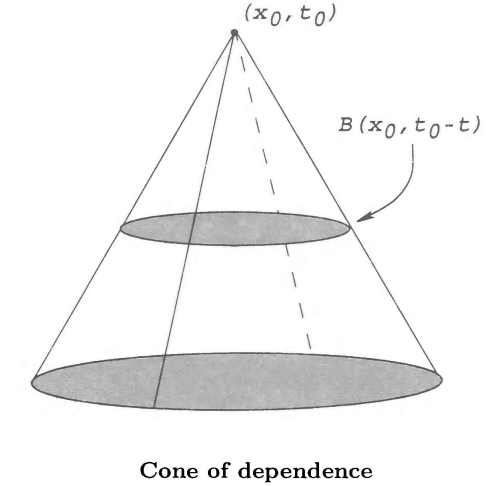
\includegraphics[width=0.4\textwidth]{cone.png}
\end{figure}
\begin{theorem}
(Finite propagation speed). If $u\equiv u_t\equiv0$ on $B(x_0,t_0)\times\{t=0\}$, then $u \equiv0$ within the cone $K(x_0,t_0)$.
\end{theorem}
\begin{remark}
We see that any "disturbance" originating outside $B\left(x_0, t_0\right)$ has no effect on the solution within $K(x_0,t_0)$ and consequently has finite propagation speed. We already know this from the representation formulas of Theorem \ref{thm2.28} and Theorem \ref{thm2.29}, at least assuming $g=u$ and $h=u_t$ on $\mr^n\times\{t=0\}$ are sufficiently smooth.
\end{remark}
\begin{proof}
Define the local energy
\[e(t):=\frac{1}{2}\int_{B(x_0,t_0-t)}u_t^2(x,t)+|Du(x,t)|^2\dif x(0\leq t\leq t_0).\] Then\[\begin{aligned}
	e^\prime(t)=&\int_{B(x_0,t_0-t)}u_tu_{tt}+Du\cdot Du_t\dif x-\frac{1}{2} \int_{\ptl B(x_0,t_0-t)}u_t^2+|Du|^2\dif S\\
	=&\int_{B(x_0,t_0-t)}u_t(u_{tt}-\Delta u)\dif x+\int_{\ptl B(x_0,t_0-t)}\frac{\ptl u}{\ptl\nu}u_t\dif S-\frac{1}{2}\int_{\ptl B(x_0,t_0-t)} u_t^2+|Du|^2\dif S\\
	=&\int_{\ptl B(x_0,t_0-t)}\frac{\ptl u}{\ptl\nu}u_t-\frac{1}{2}u_t^2-\frac{1}{2}|Du| ^2\dif S.
\end{aligned}\]Now\[\left|\frac{\ptl u}{\ptl\nu}u_t\right|=|(Du\cdot\bm{\nu}) u_t|\leq|Du||u_t|\leq\frac{1}{2}u_t^2+\frac{1}{2}|Du|^2\]by the Cauchy-Schwarz and Cauchy inequalities. Hence $e^\prime(t)\leq0$, and so $e(t)\leq e(0)=0(0\leq t\leq t_0)$. Thus $u_t,Du\equiv0$, and consequently $u\equiv0$ within the cone $K(x_0,t_0)$.
\end{proof}

\newpage
\subsection{Summary}
The following table is a brief summary of the last three equations in this chapter.
\begin{table}[h]
	\centering
	\begin{tabular}{|c|c|c|c|c|}
		\hline
		& \multicolumn{1}{c|}{Type} & M-V property & \multicolumn{1}{c|}{Maximum princ.} & Smoothness \\ \hline
		Laplace's equation & \multicolumn{1}{c|}{Elliptic} & Theorem \ref{MVF1} & \multicolumn{1}{c|}{Theorem \ref{2.4}} & Theorem \ref{thm2.6} \\ \hline
		Heat equation & \multicolumn{1}{c|}{Parabolic} & Theorem \ref{thm2.205} & \multicolumn{1}{c|}{Theorem \ref{thm2.20}} & Theorem \ref{thm2.25} \\ \hline
		Wave equation & \multicolumn{1}{c|}{Hyperbolic} & -- & \multicolumn{1}{c|}{--} & {\color{red} Loss of regularity} \\ \hline\hline
		\multicolumn{1}{|l|}{} & \multicolumn{2}{c|}{Uniqueness of Cauchy prob.} & \multicolumn{2}{c|}{Some other properties} \\ \hline
		Laplace's equation & \multicolumn{2}{c|}{Theorem \ref{thm2.5}} & \multicolumn{2}{c|}{Theorem \ref{Liou}, \ref{thm2.10}, \ref{thm2.11}} \\ \hline
		Heat equation & \multicolumn{2}{c|}{Theorem \ref{thm2.21}, \ref{thm2.23}} & \multicolumn{2}{c|}{Inf. prop. speed; no time reversal} \\ \hline
		Wave equation & \multicolumn{2}{c|}{--} & \multicolumn{2}{c|}{Finite prop. speed; time reversal} \\ \hline
	\end{tabular}
\end{table}


\newpage
\subsection{Problems}
In the following exercises, all given functions are assumed smooth, unless otherwise stated.
\begin{problem}\label{prob1}
Write down an explicit formula for a function $u$ solving the initial-value problem
\[\left\{\begin{aligned}
	u_t+b\cdot Du+cu & =0 & & \text{in~}\mr^n\times(0,\infty) \\
	u & =g & & \text{on~}\mr^n\times\{t=0\}.
\end{aligned}\right.\]
Here $c\in\mr$ and $b\in\mr^n$ are constants.
\end{problem}
\begin{proof}
Fix $x\in\mr^n$ and $t\in(0,+\infty)$ and consider $z(s):=u(x+bs,t+s)$ for $s\in\mr$. Then we have \[\dot{z}(s)=b\cdot Du(x+bs,t+s)+u_t(x+bs,t+s)=-cu(x+bs,t+s)=-cz(s).\]
Now the PDE reduces to an ODE, and solving the equation $\dot{z}(s)=-cz(s)$ gives $z(s)=D\e^{-cs}$ for some constant $D$. To solve $D$ we let $s=-t$, and \[z(-t)=u(x-tb,0)= g(x-tb)=D\e^{ct}.\]Therefore $D=g(x-tb)\e^{-ct}$. Thus, $u(x+bs,t+s)=g(x-tb)\e^{-ct-cs} $, and letting $s=0$ implies that $u(x,t)=g(x-tb)\e^{-ct}$.
\end{proof}
\begin{problem}\label{prob2}
Prove that Laplace's equation $\Delta u=0$ is rotation invariant; that is, if $O$ is an orthogonal $n\times n$ matrix and we define\[v(x):=u(Ox)(x\in\mr^n),\] then $\Delta v=0$.
\end{problem}
\begin{proof}
\textsf{An abstract proof.} We shall use some properties of gradient and divergence, and the fact that the Laplacian of $f$ is $\Delta f=\dv\cdot\nabla f$. Note that\[\begin{aligned}
	\Delta v(x)&=(\dv\cdot\nabla)v(x)=(\dv\cdot\nabla)u(Ox)\\
	&=\dv(O(\nabla u)(Ox))=O^\T(\dv(O\nabla u))(Ox)\\
	&=O^\T O(\dv\cdot\nabla)(u)(Ox)\\
	&=\Delta u(Ox)=0.
\end{aligned}\]\\
\textsf{A brief proof.} Write $O=(a_{ij})$ and by chain rule we have \[v_{x_i}(x)=\sum_{k=1}^nu_{x_k}(Ox)a_{ki}.\]Thus \[v_{x_ix_i}(x)= \sum_{k=1}^na_{ki}\left(\sum_{l=1}^nu_{x_kx_l}(Ox)a_{li}\right)=\sum_{k=1}^n\sum_{l=1}^na_{ki}a_{li}u_{x_kx_l}(Ox).\]Since $O$ is orthogonal, we have $O^\T O=I$, i.e. \[\sum_{i=1}^na_{ki}a_{li}=\left\{\begin{array}{c}
	1, \text{ if } k=l \\
	0, \text{ if } k\neq l
\end{array}\right.\]Thus the Laplacian of $v$ is \[\begin{aligned}
	\Delta v(x)&=\sum_{i=1}^n\sum_{k=1}^n\sum_{l=1}^na_{ki}a_{li}u_{x_kx_l} (Ox)=\sum_{k=1}^n\sum_{l=1}^n\left(u_{x_kx_l}(Ox)\sum_{i=1}^na_{ki}a_{li}\right)\\ &=\sum_{k=1}^nu_{x_kx_k}(Ox)\cdot1=\Delta u(Ox)=0,
\end{aligned}\]as desired.\\
\textsf{A detailed proof.} Let $y:=Ox$ and $O=(a_{i j})$ as above. Thus,\[v(x)=u(Ox)=u(y)\]where $y_j=\dis\sum_{i=1}^na_{ji}x_i$. This then gives that\[v_{x_i}=\sum_{j=1}^nu_{y_j}\frac{\ptl y_j}{\ptl x_i}=\sum_{j=1}^nu_{y_j}a_{ji}.\]Thus\[\begin{aligned}
	\begin{pmatrix}
		v_{x_1}\\
		\vdots \\
		v_{x_n}
	\end{pmatrix}
	&=\begin{pmatrix}
		a_{11} & \cdots & a_{n1} \\
		\vdots & & \vdots \\
		a_{1n} & \ldots & a_{n n}
	\end{pmatrix}
	\begin{pmatrix}
		\frac{\ptl u}{\ptl y_1} \\
		\vdots \\
		\frac{\ptl u}{\ptl y_n}
	\end{pmatrix}=O^\T\begin{pmatrix}
		\frac{\ptl u}{\ptl y_1} \\
		\vdots \\
		\frac{\ptl u}{\ptl y_n}
	\end{pmatrix}\\
	\implies D_xv &=O^\T D_yu.
\end{aligned}\]
Now,\[\begin{aligned}
	\Delta v &=D_xv\cdot D_xv\\
	&=(O^\T D_yu)\cdot(O^\T D_yu)=(O^\T D_yu)^\T O^\T D_yu \\
	&=(D_yu)^\T(O^\T)^\T O^\T D_yu=(D_yu)^\T OO^\T D_yu \\
	&=(D_yu)^\T D_yu\quad\text{ because } O \text{ is orthogonal } \\
	&=(D_yu)\cdot(D_yu)=\Delta u(y)=0.
\end{aligned}\]Hence we finish the proof.
\end{proof}
\begin{problem}
Modify the proof of the mean-value formulas to show for $n\geq3$ that
\[u(0)=\dashint_{\ptl B(0,r)}g\dif S+\frac{1}{n(n-2)\alpha(n)}\int_{B(0,r)} \left(\frac{1}{|x|^{n-2}}-\frac{1}{r^{n-2}}\right)f\dif x\]
provided\[\left\{\begin{aligned}
	-\Delta u=f &\text{\;~~in~}B^0(0,r) \\
	u=g &\text{\;~~on~}\ptl B(0,r)
\end{aligned}\right.\]
\end{problem}
\begin{proof}
Define\[\phi(s):=\dashint_{\ptl B(0,s)}u(y)\dif S(y)=\dashint_{\ptl B(0,1)}u(sz)\dif S(z),\] and we shall have\[\begin{aligned}
	\phi^\prime(s)&=\dashint_{\ptl B(0,1)}Du(sz)\cdot z\dif S(z)=\frac{1} {n\alpha(n)s^{n-1}}\int_{\ptl B(0,s)}Du(y)\,\frac{y}{s}\,\dif S(y)\\
	&=\frac{1}{n\alpha(n)s^{n-1}}\int_{\ptl B(0,s)}\frac{\ptl u}{\ptl\nu}\dif S(y)\xlongequal{\text{Green's formula}}\frac{s}{n}\frac{1}{\alpha(n)s^n}\int_{B(0,s)} \Delta u(y)\dif y\\&=\frac{s}{n}\dashint_{B(0,s)}\Delta u(y)\dif y.\end{aligned}\]Let $\ve>0$ be given, and using integration by parts we get\[\begin{aligned}
	&\phi(\ve)-\phi(r)=-\int_\ve^r\phi^\prime(s)\dif s\\
	&=\int_\ve^r\left(\frac{s}{n}\dashint_{B(0,s)}f(y)\dif y\right)\dif s\quad\text{ because }\Delta u(y)=-f(y)\\&=\int_\ve^r\left(\frac{1}{n\alpha(n)s^{n-1}} \int_{B(0,s)}f(y)\dif y\right)\dif s=\frac{1}{n\alpha(n)}\int_\ve^r\frac{1}{s^{n-1}}\int_{B(0,s)}f(y)\dif y\dif s\\
	&\xlongequal{\text{Appendix \ref{polar}.3}}\frac{1}{n\alpha(n)} \left(\left.\frac{1}{(2-n)s^{n-2}}\int_{B(0,s)}f(y)\dif y\right|_\ve^r -\int_\ve^r\frac{1}{(2-n)s^{n-2}}\int_{\ptl B(0,s)}f(y)\dif S(y)\dif s\right)\\
	&=\frac{1}{n(n-2)\alpha(n)}\left(\int_\ve^r\frac{1}{s^{n-2}}\int_{\ptl B(0,s)}f(y)\dif S(y)\dif s-\frac{1}{r^{n-2}}\int_{B(0,r)}f(y)\dif y+\frac{1}{\ve^{n-2}}\int_{B(0,\ve)}f(y)\dif y\right)\\
	&=:\frac{1}{n(n-2)\alpha(n)}\left(I-\frac{1}{r^{n-2}}\int_{B(0,r)}f(y)\dif y+J\right).
\end{aligned}\]
Observe that\[|J|\leq\frac{1}{\ve^{n-2}}|B(0,\ve)|\cdot\|f(y)\|_{L^\infty (\overline{B(0,r)})}\leq C\ve^2\quad\text{for some constant~} C>0\]and\[\int_0^r \frac{1}{s^{n-2}}\dif s\int_{\ptl B(0,s)}f(y)\dif S(y)=\int_0^r\int_{\ptl B(0,s)} \frac{f(y)}{s^{n-2}}\dif S(y)\dif s=\int_{B(0,r)}\frac{f(x)} {|x|^{n-2}}\dif x.\]As $\ve\to0$ we have\[I+J\to\int_{B(0,r)}\frac{1}{|x|^{n-2}}f(x)\dif x.\]
Thus\[\begin{aligned}
	\lim_{\ve\to0}\phi(\ve)-\phi(r)&=-\lim_{\ve\to0}\int_\ve^r\phi^\prime(s)\dif s\\
	&=\frac{1}{n(n-2)\alpha(n)}\left(\int_{B(0,r)}\frac{1}{|x|^{n-2}}f(x)\dif x-\frac{1}{r^{n-2}}\int_{B(0,r)}f(y)\dif y\right)\\
	&=\frac{1}{n(n-2)\alpha(n)}\int_{B(0,r)}\left(\frac{1}{|x|^{n-2}}-\frac{1}{r^{n-2}}\right)f(x)\dif x.
\end{aligned}\]Moreover, note that \[\lim_{\ve\to0}\phi(\ve)=\lim_{\ve\to0}\frac{1}{|\ptl B(0,\ve)|} \int_{\ptl B(0,\ve)}u(y)\dif S(y)=u(0),\]which is given by the last formula of Theorem \ref{thm2.1}. Finally, we calculate
\[\begin{aligned}
	u(0)&=\phi(r)+\frac{1}{n(n-2)\alpha(n)}\int_{B(0,r)}\left(\frac{1}{|x|^{n-2}}-\frac{1}{r^{n-2}}\right)f(x)\dif x\\
	&=\dashint_{\ptl B(x,r)}u(y)\dif S(y)+\frac{1}{n(n-2)\alpha(n)}\int_{B(0,r)} \left(\frac{1}{|x|^{n-2}}-\frac{1}{r^{n-2}}\right)f(x)\dif x\\
	&=\dashint_{\ptl B(0,r)}g\dif S+\frac{1}{n(n-2)\alpha(n)}\int_{B(0,r)} \left(\frac{1}{|x|^{n-2}}-\frac{1}{r^{n-2}}\right) f\dif x,
\end{aligned}\]so we are done.
\end{proof}
\begin{problem}\label{prob2.4}
Give a direct proof that if $u\in C^2(U)\cap C(\bar{U})$ is harmonic within a bounded open set $U$, then\[\max_{\bar{U}}u=\max_{\ptl U}u.\]
(Hint: Define $u_\ve:=u+\ve|x|^2$ for $\ve>0$, and show $u_\ve$ cannot attain its maximum over $\bar{U}$ at an interior point.)
\end{problem}
\begin{proof}
As per the hint, define $u_\ve:=u+\ve|x|^2$, and clearly $u<u_\ve$ for all $\ve>0$. Since $\ptl_{x_i}|x|^2=2x_i$ and $u$ is harmonic, we have \[\Delta u_\ve=0+2n\ve>0\quad\text{for } x\in U.\] As $u_\ve$ is continuous on the bounded and closed $\bar{U},u_\ve$ can achieve its maximum and minimum on $\bar{U}$. Now for sake of contradiction, suppose that $u_\ve$ attains its maximum at an interior point $x_0$ of $U$. Analysis tells us that $D^2u_\ve(x_0)=\hess(u_\ve(x_0))$ is negative semi-definite and algebra gives that the trace of a negative semi-definite matrix is non-positive, causing a clear contradiction since \[0\geq\tr(D^2u_\ve(x_0))=\Delta u_\ve(x_0)>0.\]
Therefore, $x_0$ cannot be local maximum of $u_\ve$, so we conclude that \[\max_{\bar{U}}u_\ve=\max_{\ptl U}u_\ve.\]
We assume $\bar{U}\subset B(0,R)$ for some $R>0$ since $U$ is bounded. Then\[\max_ {\bar{U}}u\leq\max_{\bar{U}}u_\ve=\max_{\ptl U}u_\ve\leq\max_{\ptl U}u+\max_ {\ptl U}\ve|x|^2\leq\max_{\ptl U}u+\ve R^2.\]By letting $\ve\to0$ we get $\max\limits_ {\bar{U}}u\leq\max\limits_{\ptl U}u$. Finally, since $\ptl U\subset\bar{U}$, we conclude that $\max\limits_{\bar{U}}u=\max\limits_{\ptl U}u$, proving the result.
\end{proof}
\begin{problem}
We say $v\in C^2(\bar{U})$ is \textit{subharmonic} if\[-\Delta v\leq0\text{ ~in }U.\]
(a) Prove for subharmonic $v$ that
\[v(x)\leq\dashint_{B(x,r)}v\dif y~\text{ for all } B(x,r)\subset U.\]
(b) Prove that therefore $\max\limits_{\bar{U}}v=\max\limits_{\ptl U}v$.\\
(c) Let $\phi:\mr\to\mr$ be smooth and convex. Assume $u$ is harmonic and $v:=\phi(u)$. Prove $v$ is subharmonic.\\
(d) Prove $v:=|Du|^2$ is subharmonic, whenever $u$ is harmonic.
\end{problem}
\begin{proof}
(a) The proof starts out being essentially the same as the mean-value formulas for harmonic functions. Set \[\phi(r):=\dashint_{\ptl B(x,r)}v(y)\dif S(y)\] and we obtain as in Theorem \ref{MVF1} \[\phi^\prime(r)=\frac{r}{n}\dashint_{B(x,r)}\Delta v(y)\dif y\geq0.\]For $0<\ve<r$,\[\int_\ve^r\phi^\prime(s)\dif s=\phi(r)-\phi(\ve)\geq0.\]Similarly, we have $v(x)=\limls_{\ve\to0}\phi(\ve)\leq\phi(r)$. Therefore,\[\begin{aligned}
	&\dashint_{B(x,r)}v(y)\dif y=\frac{1}{\alpha(n)r^n}\int_{B(x,r)}v(y)\dif y= \frac{1}{\alpha(n)r^n}\int_0^r\left(\int_{\ptl B(x,s)}v(z)\dif S(z)\right)\dif s\\
	=&\frac{1}{\alpha(n)r^n}\int_0^rn\alpha(n)s^{n-1}\phi(s)\dif s\geq\frac{1}{r^n} \int_0^rns^{n-1}v(x)\dif s=v(x).
\end{aligned}\]
(b) We only need to make a tiny change to the proof of the maximum principle. Suppose $U$ is connected and there exists a point $x_0\in U$ with $v(x_0)=M:=\max\limits_{\bar{U}} v$. Then, for $0<r<d(x_0,\ptl U)$, use the result of part (a):\[M=v(x_0)\leq\dashint_ {B(x_0,r)} v(y)\dif y\leq M,\]which then forces $v(y)\equiv M$ for all $y\in B(x_0,r)$. Hence the set $S=\{x\in U:v(x)=M\}$ is both open (because every point of $S$ is an interior point) and relatively closed (because $v$ is continuous) in $U$ and thus equals $U$ since $U$ is connected. Hence $v$ is constant in $U$ and also in $\bar{U}$ since $v$ is continuous, and we conclude that $\max\limits_{\bar{U}}v=\max\limits_{\ptl U}v$.\\[4pt]
Now let $\{U_i:i\in I\}$ be the connected components of $U$. Pick any $x\in U$ and find $j\in I$ such that $x\in U_j$. We then obtain\[v(x)\leq\max_{\bar{U}_j}v=\max _{\ptl U_j}v\leq\max_{\ptl U}v\]for all $x\in U$ and the result follows.\\[4pt]
(c) Convexity and smoothness of $\phi$ implies that $\phi^{\prime\prime}\geq0$. Now straight calculations show that\[\begin{gathered}
	v_{x_i}=\frac{\ptl\phi}{\ptl u}u_{x_i},v_{x_ix_j}=\frac{\ptl^2\phi} {\ptl u^2}u^2_{x_i}+\frac{\ptl\phi}{\ptl u}u_{x_ix_j}\\ \implies\Delta
	v=\sum_{i=1}^nv_{x_ix_i}=\frac{\ptl^2\phi}{\ptl u^2}\sum_{i=1}^nu^2 _{x_i}+\frac{\ptl\phi}{\ptl u}\Delta u= \phi^{\prime\prime}|Du|^2\geq0,
\end{gathered}\]implying that $v$ is subharmonic.\\[4pt]
(d) \textsf{Proof 1}. First note that $v=|Du|^2=\dis\sum_{i=1}^nu_{x_i}^2$, and so \[\begin{gathered}
	v_{x_j}=2\sum_{i=1}^nu_{x_i}u_{x_ix_j},v_{x_jx_j}=2\sum_{i=1}^n(u^2_{x_ix_j}+u_{x_i}u_{x_ix_jx_j})\\ \implies\frac{1}{2}\Delta
	v=\sum_{j=1}^n\sum_{i=1}^n(u^2_{x_ix_j}+u_{x_i}u_{x_ix_jx_j})=\sum_{j=1}^n\sum_{i=1}^nu^2_{x_ix_j}+\sum_{i=1}^nu_{x_i}(\Delta u)_{x_i}\geq0.
\end{gathered}\]By definition $v$ is subharmonic.\\[4pt]
\textsf{Proof 2}. We know that if $u$ is harmonic, $u_{x_i}$ is harmonic. Moreover, $u^2_{x_i}$ is convex with respect to $u_{x_i}$, so from (c) we know that $(u_{x_i})^2$ is subharmonic. Obviously the sum of subharmonic functions is still subharmonic, so $v=|Du|^2=\dis\sum_{i=1}^n(u_{x_i})^2$ is subharmonic.
\end{proof}
\begin{problem}
Let $U$ be a bounded, open subset of $\mr^n$. Prove that there exists a constant $C$, depending only on $U$, such that
\[\max_{\bar{U}}|u|\leq C(\max_{\ptl U}|g|+\max_{\bar{U}}|f|)\]
whenever $u$ is a smooth solution of\[\left\{\begin{aligned}
	-\Delta u=f &\text{~ in }U\\
	u=g &\text{~ on }\partial U .
\end{aligned}\right.\]
(Hint: $-\Delta(u+\dfrac{|x|^2}{2n}\lambda)\leq0$, for $\lambda:=\max\limits_{\bar{U}}|f|.$)
\end{problem}
\begin{proof}
Suppose that $f$ is bounded on $\bar{U}$ (otherwise the inequality naturally holds). Now following the hint, we consider the function $v(x):=u(x)+\frac{|x|^2}{2n}\lambda$, where $\lambda:=\max\limits _{\bar{U}}|f|$. Then we calculate \[\Delta v=\Delta u+n\frac{2}{2n}\lambda=\lambda-f\geq0,\]implying that $v$ is subharmonic. Since $U$ is bounded, $M:=\max\limits_{\bar{U}}|x|^2$ exists and is finite. The weak maximum principle as in the previous problem which holds for subharmonic functions gives that
\[\max_{\bar{U}}u\leq\max_{\bar{U}}v=\max_{\partial U}v\leq\max_{\ptl U}|g|+ \frac{M}{2n}\max_{\bar{U}}|f|.\]Replacing $u$ by $-u$ in $v$ and we have \[\max_{\bar{U}}-u\leq\max_{\bar{U}}v=\max_{\ptl U}v\leq\max_{\ptl U}|g|+ \frac{M}{2n}\max_{\bar{U}}|f|.\] Combine the two equations above and set $C:=\max\{1, M\}$, and we have\[\max_{\bar{U}}|u|\leq C(\max_{\ptl U}|g|+\max_{\bar{U}}|f|).\] Finally, since $M$ only depends on $U$, we see that $C$ does as well.
\end{proof}
\begin{problem}
Use Poisson's formula for the ball to prove
\[r^{n-2}\frac{r-|x|}{(r+|x|)^{n-1}}u(0)\leq u(x)\leq r^{n-2}\frac{r+|x|}{(r-|x|)^{n-1}}u(0)\]
whenever $u$ is positive and harmonic in $B^0(0,r)$. This is an explicit form of Harnack's inequality.
\end{problem}
\begin{proof}
First recall Poisson's formula for the ball:\[u(x)=\frac{r^2-|x|^2}{n\alpha(n)r}\int_{\ptl B(0,r)} \frac{g(y)}{|x-y|^n}\dif S(y)~(x\in B^0(0,r))\]solves $\Delta u=0$ in $B^0(0,r)$ and $u=g$ on $\partial B(0,r)$. Second, the triangle equality $|y|-|x|\leq|x-y|\leq|x|+|y|$ gives \[\frac{1}{(r+|x|)^n} \leq\frac{1}{|x-y|^n}\leq\frac{1}{(r-|x|)^n}\]for every $y$ on $\ptl B(0,r)$ and $x$ in $B^0(0,r)$. Now combining the two equations above we obtain (taking the first half of the inequality as an example)\[\begin{aligned}
	u(x)&=\frac{(r+|x|)(r-|x|)}{n\alpha(n)r}\int_{\ptl B(0,r)}\frac{g(y)}{|x-y|^n}\dif S(y)\\
	&\geq\frac{(r+|x|)(r-|x|)}{n\alpha(n)r}\int_{\ptl B(0,r)}\frac{g(y)}{(r+|x|)^n}\dif S(y)=\frac{(r-|x|)r^{n-2}}{n\alpha(n)r^{n-1}(r+|x|)^{n-1}}\int_{\ptl B(0,r)}g(y)\dif S(y)\\
	&=r^{n-2}\frac{r-|x|}{(r+|x|)^{n-1}}\dashint_{\ptl B(0,r)}g(y)\dif S(y)=r^{n-2}\frac{r-|x|}{(r+|x|)^{n-1}}\dashint_{\ptl B(0,r)}u(y)\dif S(y)\\
	&\xlongequal{\text{mean-value formula}}r^{n-2}\frac{r-|x|}{(r+|x|)^{n-1}}u(0).
\end{aligned}\]The proof of the second part is exactly the same.
\end{proof}
\begin{problem}
Prove Theorem \ref{thm2.14.5}. (Hint: Since $u\equiv1$ solves $\left\{\begin{aligned} \Delta u=0 &\quad\text{in } B^0(0,r)\\ u=g &\quad\text{on } \ptl B(0,r)\end{aligned}\right.$ for $g\equiv1$, the theory automatically implies
\[\int_{\ptl B(0,1)}K(x,y)\dif S(y)=1\]for each $x\in B^0(0,1)$.)
\end{problem}
\begin{proof}
(i) First recall that \[\tag{64}\label{64}u(x)=\dis\int_{\ptl B(0,r)}K(x,y)g(y)\dif S(y).\]
 By definition, $G(x,y)$ is smooth and harmonic for $x\neq y$, and hence, given $\ve>0$, there exists $\delta>0$ such that \[|D^\alpha K(x,y)-D^\alpha K(x_0,y)|<\ve\] for derivatives of any order whenever $|x-x_0|<\delta$ (this statement is equivalent to the continuity of $D^\alpha K(x,y)$). Since $\ptl B(0,r)$ is compact, we see that \[D^\alpha u(x)=\int_{\ptl B(0,r)}D_x^\alpha K(x,y)g(y)\dif y.\]This is done 
through the mean value theorem (see Theorem 9.42 of \emph{Principles of Mathematical Analysis} by Rudin) or the dominated convergence theorem(see Theorem 2.27 of \emph{Real Analysis} by Folland). Noting that $g$ is bounded since it is continuous on a compact set, we obtain\[\begin{aligned}
	\left|D^\alpha u(x)-D^\alpha u(x_0)\right|&\leq\int_{\ptl B(0,r)}|D^\alpha K(x,y)-D^\alpha K(x_0,y)\|g(y)|\dif y\\
	&<\ve\int_{\ptl B(0,r)}|g(y)|\dif y\\
	&\leq n\alpha(n)\ve\|g\|_{L^\infty(\ptl B(0,r))}\to0~\text{as}~x\to x_0.
\end{aligned}\]Hence $u$ is smooth.\\
(ii) It is clear by the above that \[\Delta u(x)=\int_{\ptl B(0,r)}\Delta_x K(x,y)g(y)\dif y=0.\]
(iii) In this section we are to show that $\limls_{x\to x_0}u(x)=g(x_0)$ for arbitrary $x_0 \in\ptl B(0,r)$. We will conduct a similar process as in the proof of Theorem \ref{thm2.14}. Fix $x_0\in\ptl B(0,r),\ve>0$. Choose sufficiently small $\delta>0$ so that $|g(y)-g(x_0)|<\ve$ whenever $|y-x_0|<\delta,y\in B(0,r)$. Moreover, since $g$ is defined in a bounded compact set $B(0,r)$, it is also bounded, and thus we assume that $|g(y)|<M$. Now equation (\ref{64}) in (i) gives that\[\begin{aligned}
	|u(x)-g(x_0)|&=\left|\int_{\ptl B(0,r)}g(y)K(x,y)\dif S(y)-\int_{\ptl B(0,r)}g(x_0)K(x, y)\dif S(y)\right|\\
	&=\left|\int_{\ptl B(0,r)}(g(y)-g(x_0))K(x,y)\dif S(y)\right|\\
	&\leq\int_{\ptl B(0,r)}|g(y)-g(x_0)|K(x,y)\dif S(y)\\
	&=\int_{\ptl B(0,r)\cap B(x_0,\delta)}|g(y)-g(x_0)|K(x,y)\dif S(y)+\\
	&\qquad\int_{\ptl B(0,r)-B(x_0,\delta)}|g(y)-g(x_0)|K(x,y)\dif S(y)\\
	&=:I+J.
\end{aligned}\]Again by (\ref{64}) we have \[I<\int_{\ptl B(0,r)\cap B(x_0,\delta)}\ve K(x,y)\dif S(y)<\ve\int_{\ptl B(0,r)}K(x,y)\dif S(y)=\ve.\]Furthermore, if $|x-x_0|<\delta/2$ and $|y-x_0|>\delta$, then\[|y-x_0|<|y-x|+|x-x_0|<|y-x|+ \frac{\delta}{2}<|y-x|+\frac{1}{2} |y-x_0|,\] which is $|y-x|>|y-x_0|/2$. So\[K(x,y)= \frac{r^2-|x|^2}{n\alpha(n)r|x-y|^n}<\frac{2^n(r^2-|x|^2)}{n\alpha(n)r}\frac{1}{|y-x_0|^n}<\frac{2^n(r^2-|x|^2)}{n\alpha(n)r\delta^n}\]for $|x-x_0|<\delta/2$ and $y\in\ptl B(0,r)-B(x_0,\delta)$. By the triangle inequality, we have $|g(y)-g(x_0)|<2M$. Consequently\[\begin{aligned}
	J&=\int_{\ptl B(0,r)-B(x_0,\delta)}|g(y)-g(x_0)|K(x,y)\dif S(y)\\&<2M\int_{\ptl B(0,r)- B(x_0,\delta)}\frac{2^n(r^2-|x|^2)}{n\alpha(n)r\delta^n}\dif S(y)\leq2M \frac{2^n(r^2-|x|^2)}{n\alpha(n)r\delta^n}n\alpha(n)r^n\\
	&=(r^2-|x|^2)\frac{2^{n+1}Mr^{n-1}}{\delta^n}\to0\quad(|x|\to r\text{~as~}x\to x_0\in\ptl B(0,r)).\end{aligned}\]Finally we conclude that $|u(x)-g(x_0)|\to 0$ as $x\to x_0$, as desired.
\end{proof}
\begin{problem}
Let $u$ be the solution of\[\left\{\begin{aligned}
	\Delta u=0 &\text{~ in }\mr_+^n\\
	u=g &\text{~ on }\ptl\mr_+^n
\end{aligned}\right.\]
given by Poisson's formula for the half-space. Assume $g$ is bounded and $g(x)=|x|$ for $x \in \ptl\mr_{+}^n$, $|x|\leq1$. Show $Du$ is \textit{not} bounded near $x=0$. (Hint: Estimate $\frac{u(\lambda e_n)-u(0)}{\lambda}.$)
\end{problem}
\begin{proof}
According to Poisson's formula (\ref{26}) for half-plane, we have \[u(x)=\frac{2x_n}{n\alpha(n)}\int_{\ptl\mr_+^n}\frac{g(y)}{|x-y|^n}\dif y.\]Consider\[\begin{aligned}
	&\frac{u(\lambda e_n)-u(0)}{\lambda}=\frac{2}{n\alpha(n)}\int_{\ptl\mr_{+}^n} \frac{g(y)}{|\lambda e_n-y|^n}\dif y\\
	=&\frac{2}{n\alpha(n)}\int_{\ptl\mr_{+}^n\cap\{|y|\leq1\}} \frac{|y|}{(\lambda^2+|y|^2)^{n/2}}\dif y+\frac{2}{n\alpha(n)}\int_{\ptl \mr_{+}^n\cap\{|y|>1\}}\frac{g(y)}{(\lambda^2+|y|^2)^{n/2}}\dif y\\
	\geq&\frac{2}{n\alpha(n)}\int_{B(0,1)}\frac{|y|}{(\lambda^2+|y|^2)^{n/2}}\dif y.
\end{aligned}\]According to the Monotone convergence theorem, we have \[\lim_{\lambda\to0}\int_{B(0,1)}\frac{|y|}{(\lambda^2+|y|^2)^{n/2}}\dif y=\int_{B(0,1)}\frac{|y|}{|y|^n}\dif y=\infty\]This implies that $u_{x_n}(\lambda e_n)\to\infty$ as $\lambda\to0$. Hence $Du$ is not bounded near $x=0$.
\end{proof}
\begin{problem}
(Reflection principle)\\
(a) Let $U^+$ denote the open half-ball $\{x\in\mr^n:|x|<1,x_n>0\}$. Assume $u\in C^2(\overline{U^+})$ is harmonic in $U^+$, with $u=0$ on $\ptl U^+\cap\{x_n=0\}$. Set
\[v(x):=\begin{cases}u(x)& \text{ if } x_n\geq0\\-u(x_1,\cdots,x_{n-1},-x_n) & \text{ if } x_n<0\end{cases}\]
for $x\in U=B^0(0,1)$. Prove $v\in C^2(U)$ and thus $v$ is harmonic within $U$.\\
(b) Now assume only that $u\in C^2(U^+)\cap C(\overline{U^+})$. Show that $v$ is harmonic within $U$. (Hint: Use Poisson's formula for the ball.)
\end{problem}
\begin{proof}
(a) We can directly calculate $\Delta v=0$ when $|x_n|>0$. Now it suffices to prove that $D^2v$ exists when $|x_n|=0$ and $\Delta v=0$ on $\{x_n=0\}$. First we assert that for any $x_0\in\{x_n=0\},n>k$, we have\[\lim_{x_n>0,x\to x_0}v_{x_nx_k}(x)= \lim_{x_n<0,x\to x_0}v_{x_nx_k}(x)\]since $u \in C^2(\overline{U^+})$.\\
Using the continuity of $D^2u$ again, we obtain\[\sum_{i=1}^{n-1}\frac{\ptl^2}{\ptl x_i^2}u(x_0)+\frac{\ptl^2}{\ptl\nu^2}u(x_0)=\lim _{x_n>0,x\to x_0}\Delta u(x)=0.\] Additionally we know that $u_{x_ix_i}(x_0)=0$ for $1\leq i\leq n-1$, and thus $\dfrac{\ptl^2}{\ptl\nu^2}u(x_0)=0$ where $\nu=-e_n$. Consequently $\dfrac{\ptl^2}{\ptl\nu^2}v(x_0)=0$, where $\nu=e_n$ or $-e_n$, which is equivalent to $v_{x_nx_n}(x_0)=0$. Then we have $\Delta v(x_0)=0$, implying that $v$ is harmonic and $v\in C^2(U)$.\\
(b) We employ Poisson's formula for the ball to find that
\[v(x)=\int_{\ptl B(0,1)}K(x,y)v(y)\dif S(y),\]where $K(x,y)$ denotes Poisson's kernel. We have shown that $K$ is harmonic and that $K(x,y)\in C^2(\overline{B(0,1)})$, and so we find that\[\frac{\ptl v(x)}{\ptl x_i}=\int_{\ptl B(0,1)}\frac{\ptl K(x, y)}{\ptl x_i}v(y)\dif S(y).\]Since $v$ is continuous on $\ptl B(0,1)$, we see that $\dfrac{\ptl K(x,y)}{\ptl x_i}v(y)$ is continuous and hence so is the integral, and so $v(x)\in C^1(\bar{U})$.  Similarly, the second derivative is easy to calculate:\[
\frac{\ptl^2 v(x)}{\ptl x_i^2}=\int_{\ptl B(0,1)}\frac{\ptl^2K(x,y)}{\ptl x_i^2}v(y)\dif S(y)\]So that $v\in C^2(\bar{U})$. Finally, note that $K(x,y)$ is harmonic:
\[\Delta v(x)=\int_{\ptl B(0,1)}\Delta_xK(x,y)v(y)\dif S(y)=0.\]
Hence $v$ is harmonic, and we are done.
\end{proof}
\begin{problem}
(Kelvin transform for Laplace's equation) The \textit{Kelvin transform} $\mathcal{K}u=\bar{u}$ of a function $u:\mr^n\to\mr$ is
\[\bar{u}(x):=u(\bar{x})|\bar{x}|^{n-2}=u(x/|x|^2)|x|^{2-n}(x\neq 0),\]
where $\bar{x}=x/|x|^2$. Show that if $u$ is harmonic, then so is $\bar{u}$.\\
(Hint: First show that $D_x\bar{x}(D_x\bar{x})^\T=|\bar{x}|^{-4}I$. The mapping $x\to\bar{x}$ is \textit{conformal}, meaning angle preserving.)
\end{problem}
\begin{proof}
First define $\psi:\mr^n\to\mr^n$ by $\psi(x)=\bar{x}$ and compute \[\frac{\ptl}{\ptl x_i}\psi^j(x)=\frac{\delta_{ij}}{|x|^2}-\frac{2x_ix_j} {|x|^4},\]where $\delta_{ij}$ is the Kronecker symbol. Hence \[\begin{aligned}
	&D_x(\bar{x})=\left(\frac{\ptl\psi}{\ptl x_1}(x),\frac{\ptl\psi}{\ptl x_2}(x),\cdots,\frac{\ptl\psi}{\ptl x_n}(x)\right)=|x|^{-2}(I-2xx^\T/|x|^2)\\
	=&\begin{pmatrix}
		(|x|^2-2x_1^2)|x|^{-4}&-2x_1x_2|x|^{-4}&\cdots&-2x_1x_n|x|^{-4}\\
		-2x_2x_1|x|^{-4}&(|x|^2-2x_2^2)|x|^{-4}&\cdots&-2x_2x_n|x|^{-4}\\
		-2x_3x_1|x|^{-4}&-2x_3x_2|x|^{-4}&\cdots&-2x_3x_n|x|^{-4}\\
		\vdots & \vdots & \ddots & \vdots \\
		-2x_nx_1|x|^{-4}&-2x_nx_2|x|^{-4}&\cdots&(|x|^2-2x_n^2)|x|^{-4}
\end{pmatrix}\end{aligned}\]and this implies that $D_x\bar{x}(D_x\bar{x})^\T=|x|^
{-4}(I-4|x|^{-2}xx^\T+4|x|^{-4}xx^\T xx^\T)=|\bar{x}|^{-4}I$.\\
We now calculate $\Delta\psi$; since \[\psi_{x_ix_i}^j=-2|x|^{-4}(x_j+2\delta_{ij}x_i)+ 8|x|^{-6}x_i^2x_j,\]we have \[\begin{aligned}
	\Delta\psi^j&=\sum_{i=1}^n\psi_{x_ix_i}^j=\sum_{i=1}^n(-2|x|^{-4}(x_j+2\delta_{ij}x_i)+ 8|x|^{-6}x_i^2x_j)\\
	&=-2|x|^{-4}\sum_{i=1}^n(x_j+2\delta_{ij}x_i)+8|x|^{-6}x_j\sum_{i=1}^nx_i^2\\
	&=-2|x|^{-4}(n+2)x_j+8|x|^{-4}x_j=2(2-n)\frac{x_j}{|x|^4},
\end{aligned}\]implying that\[\Delta\psi=2(2-n)\frac{x}{|x|^4}.\] Therefore by applying the product rule $\Delta(uv)=u\Delta v+2\nabla u\cdot\nabla v+v\Delta u$ and calculating the composition rule\[\begin{aligned}
	&\Delta u(\psi(x))=\sum_{i=1}^n\frac{\ptl^2}{\ptl x_i^2}u(\psi(x))=\sum_{i=1} ^n\frac{\ptl}{\ptl x_i}\left(\sum_{j=1}^n\frac{\ptl}{\ptl x_j}u(\psi(x)) \cdot\frac{\ptl}{\ptl x_i}\psi^j\right)\\
	=&\sum_{i=1}^n\left(\sum_{j=1}^n \sum_{k=1}^n\frac{\ptl^2}{\ptl x_k \ptl x_j}u(\psi(x))\frac{\ptl}{\ptl x_k} u(\psi(x))\cdot\frac{\ptl}{\ptl x_k}\psi^k\cdot\frac{\ptl}{\ptl x_i}\psi^j+\sum_{j=1}^n\frac{\ptl}{\ptl x_j}u(\psi(x))\cdot\frac{\ptl^2}{\ptl x_i^2}\psi^j\right)\\
	=&\sum_{i=1}^n(D\psi^i)^\T D^2u(\psi(x))D\psi^i+Du\cdot\Delta\psi.
\end{aligned}\] we obtain
\[\begin{aligned}
	\Delta\bar{u}&=\Delta(u(x/|x|^2)|x|^{2-n})=u(\bar{x})\Delta(|x|^{2-n})+2D\bar{u}\cdot D(|x|^{2-n})+|x|^{2-n}\Delta u(\bar{x})\\ &=u(\bar{x})\Delta(|x|^{2-n})+2DuD\bar{x}(D|x|^{2-n})^\T+|x|^{2-n}(Du\cdot\Delta\bar{x}+\tr((D\bar{x})^\T D^2uD\bar{x})).
\end{aligned}\]
Note that \[\begin{aligned}
	&\Delta(|x|^{2-n})=\sum_{i=1}^n\frac{\ptl^2}{\ptl x_i\ptl x_i}|x|^{2-n}
	=\sum_{i=1}^n\frac{\ptl}{\ptl x_i}(2-n)|x|^{-n}x_i\\
	=&\sum_{i=1}^n(2-n)(-n|x|^{-2-n}x_i^2+|x|^{-n})
	=(n-2)\left(\sum_{i=1}^n\frac{nx_i^2}{|x|^{n+2}}-n\cdot\frac{1}{|x|^n}\right)=0(x\neq0)\end{aligned}\] and\[\tr((D\bar{x})^\T D^2uD\bar{x})=\tr(D\bar{x}(D\bar{x})^\T D^2u)=|x|^{-4}\Delta u=0.\]
Meanwhile, we have \[\begin{aligned}
	&2DuD\bar{x}(D|x|^{2-n})^\T=2Du\left(|x|^{-2}\left(I-2\frac{xx^\T}{|x|^2}\right)\right)(2-n)|x|^{-n}x\\=&2(n-2)|x|^{-2-n}Du\cdot x=-|x|^{2-n}Du\cdot\left(2(2-n)\frac{x} {|x|^4}\right)=-|x|^{2-n}Du\cdot\Delta\bar{x}.
\end{aligned}\]Therefore $\Delta\bar{u}=0$ and so the Kelvin transform preserves harmonic functions.
\end{proof}
\begin{problem}
Suppose $u$ is smooth and solves $u_t-\Delta u=0$ in $\mr^n\times(0,\infty)$.\\[3pt]
(a) Show $u_\lambda(x,t):=u(\lambda x,\lambda^2t)$ also solves the heat equation for each $\lambda\in\mr$.\\[3pt]
(b) Use (a) to show $v(x,t):=x\cdot Du(x,t)+2tu_t(x,t)$ solves the heat equation as well.
\end{problem}
\begin{proof}
(a) By direct calculations we have\[\begin{gathered}
	\ptl_tu_\lambda(x,t)=\lambda^2u_t(\lambda x,\lambda^2t),\\
	\ptl_{x_i}u_\lambda(x,t)=\lambda u_{x_i}(\lambda x,\lambda^2t),\ptl_{x_i}^2 u_\lambda(\lambda x,\lambda^2t)=\lambda^2u_{x_ix_i}(\lambda x,\lambda^2t),\\
	\implies\ptl_tu_\lambda-\Delta u_\lambda=\lambda^2u(\lambda x,\lambda^2 t)-\lambda^2\Delta u(\lambda x,\lambda^2t)=0.
\end{gathered}\]
(b) We derive $u_\lambda$ with respect to $\lambda$ to obtain \[\ptl_\lambda u_\lambda (x,t)=xD_xu(\lambda x,\lambda^2t)+2\lambda tu_t(\lambda x,\lambda^2t).\]Since $u$ is smooth, so is $u_\lambda$, and thus the derivatives commute. More precisely, by (a) we have \[(\ptl_t-\Delta_x)(\ptl_\lambda u_\lambda(x,t))=\ptl_\lambda(\ptl_tu_\lambda(x,t)- \Delta_xu_\lambda(x,t))=0.\]Hence $\ptl_\lambda u_\lambda(x,t)$ solves the heat equation for $\lambda\in\mr$. Set $\lambda=1$ and then $xD_xu(x,t)+2tu_t(x,t)$ solves the heat equation.
\end{proof}
\begin{problem}
Assume $n=1$ and $u(x,t)=v\left(\dfrac{x}{\sqrt{t}}\right)$.\\
(a) Show\[u_t=u_{xx}\]if and only if\begin{equation}
	v^{\prime\prime}+\frac{z}{2}v^\prime=0.\tag{$\ast$}\label{64.5}
\end{equation}
Show that the general solution of (\ref{64.5}) is\[v(z)=c\int_0^z\e^{-s^2/4}\dif s+d.\]
(b) Differentiate $u(x, t)=v\left(\dfrac{x}{\sqrt{t}}\right)$ with respect to $x$ and select the constant $c$ properly, to obtain the fundamental solution $\Phi$ for $n=1$. Explain why this procedure produces the fundamental solution. (Hint: What is the initial condition for $u$?)
\end{problem}
\begin{proof}
(a) Define $z:\mr\times\mr\to\mr$ by $z(x,t)=x/\sqrt{t}$. Then \[\begin{gathered}
	u_t(x,t)=\ptl_tv\left(\frac{x}{\sqrt{t}}\right)=-\frac{1}{2}\frac{x}{t^{3/2}} v^\prime(z(x,t))\\
	u_x(x,t)=\ptl_xv\left(\frac{x}{\sqrt{t}}\right)=\frac{1}{\sqrt{t}}v^\prime(z(x,t))\\
	u_{xx}(x,t)=\ptl_x\frac{1}{\sqrt{t}} v^\prime\left(\frac{x}{\sqrt{t}}\right)=\frac{1}{t}v^{\prime\prime}(z(x,t)).
\end{gathered}\]So \[\begin{aligned}
	&u_t=u_{xx}\\
	\iff&-\frac{1}{2}\frac{x}{t^{3/2}}v^\prime(z(x,t))=\frac{1}{t}v^\prime\prime(z(x,t))\\
	\iff&-\frac{1}{2}z(x,t)v^\prime(z(x,t))=v^{\prime\prime}(z(x,t))\\
	\iff&v^{\prime\prime}(z)+\frac{z}{2}v^\prime(z)=0.
\end{aligned}\]The last equation is exactly what we want.\\
By (\ref{64.5}) we know that $v^{\prime\prime}/v^\prime=-z/2$, and consequently, \[\ln v^\prime =\int\frac{v^{\prime\prime}}{v^\prime}+C_1=-\frac{z^2}{4}+C_1\implies v^\prime(z)=c\e^{-z^2/4},\]where $c=\e^{C_1}$ is constant. Integrate the equation above to get \[v(z)=\int_0^zv^\prime(s)\dif s+d=c\int_0^z\e^{-s^2/4}\dif s+d,\]as desired.\\
(b) It is obvious that \[v\left(\frac{x}{\sqrt{t}}\right)=c\int_0^{x/\sqrt{t}}\e^{-s^2/4}\dif s+d\]and\[u_x(x,t)=v^\prime(\frac{x}{\sqrt{t}})=\frac{c}{\sqrt{t}}\e^{-x^2/4t}.\]Now we want to integrate over $\mr$ and set the integral to 1. Thus we get \[1=\frac{c}{\sqrt{t}}\int_{-\infty}^\infty\e^{-s^2/4t}\dif s.\]But we already know that $\dis\int_{-\infty}^\infty\e^{-s^2}\dif s=\sqrt{\pi}$, and so we let $y=s/\sqrt{4t}$. Hence $\dif y=(4t)^{-1/2}\dif s$, and by substituting we obtain \[1=\frac{c}{\sqrt{t}}\int_{-\infty}^\infty\sqrt{4t}\e^{-y^2}\dif y=2c\sqrt{\pi},\]hence $c=1/(2\sqrt{\pi})$. Therefore $\Phi(x,t)=\dfrac{1}{\sqrt{4\pi t}}\e^{-x^2/4t}$.\\[3pt]
Now $u(x,t)=\dis\frac{1}{2\sqrt{\pi}}\int_0^{x/\sqrt{t}}\e^{-s^2/4}\dif s$ and we shall explain the reason why $\Phi$ defined above is the fundamental solution of the heat equation. We can analyze the behavior of $u(x,t)$ near $t=0$. The sign of $x$ matters:
\[\begin{aligned}
	&x>0:\lim_{t\to0^+}u(x,t)=\frac{1}{2\sqrt{\pi}}\int_0^\infty\e^{-\frac{s^2}{4}}\dif s=\frac{1}{\sqrt{\pi}}\int_0^\infty\e^{-s^2}\dif s=\frac{1}{2}=:u_+(x, 0), \\
	&x<0:\lim_{t\to0^+}u(x,t)=\frac{1}{2\sqrt{\pi}}\int_0^{-\infty}\e^{-\frac{s^2}{4}} d s=\frac{-1}{\sqrt{\pi}}\int_0^\infty\e^{-s^2}\dif s=-\frac{1}{2}=:u_-(x,0).
\end{aligned}\]
This shows $u(x, 0)$ is a step function with one jump at $x=0$ of height 1, and undefined at $x=0$. Now note that $u_x(x,0)$ exists and equals 0 for $x\neq0$. Now for any $\varphi\in C_c^\infty(\mr)$ we write\[\begin{aligned}
	\int_{-\infty}^{\infty}u_x(x,0)\varphi(x)\dif x&=-\int_{-\infty}^{\infty}u(x, 0) \varphi^\prime(x)\dif x=-\int_{-\infty}^0u_-(x,0)\varphi^\prime(x)\dif x-\int_0^{\infty}u_+(x, 0)\varphi^\prime(x)\dif x\\
	&=\frac{1}{2}\int_{-\infty}^0\varphi^\prime(x)\dif x-\frac{1}{2}\int_0^\infty \varphi^\prime(x)\dif x=\varphi(0)=\int_{-\infty}^\infty\delta_0(x)\varphi(x)\dif x,
\end{aligned}\]implying that $u_x(x,0)=\delta_0(x)$. This is the initial condition satisfied by the fundamental solution, hence it is no surprise that we have reached the fundamental solution.
\end{proof}
\begin{problem}
Write down an explicit formula for a solution of
\[\left\{\begin{array}{rlrl}
	u_t-\Delta u+cu=f&\text{~~in }\mr^n\times(0,\infty)\\
	u=g&\text{~~on }\mr^n\times\{t=0\},
\end{array}\right.\]
where $c\in\mr$.
\end{problem}
\begin{proof}
Set $v(x,t)=u(x,t)\e^{ct}$. Then \[v_t-\Delta v=u_t\e^{ct}+uc\e^{ct}-\e^{ct}\Delta u=\e^{ct}(u_t-\Delta u+cu)=\e^{ct}f\]and it is clear that $v=g$ on $\mr^n\times\{t=0\}$. Using Theorem \ref{thm2.18}, the function \[v(x,t)=\int_{\mr^n}\Phi(x-y,t)g(y)\dif y+\int_0^t\int_{\mr^n}\Phi(x-y,t-s)f(y,s) \e^{cs}\dif y\dif s\] solves the equation. Thus $u(x,t)=v(x,t)\e^{-ct}$ solves the system of equations.
\end{proof}
\begin{problem}
Given $g:[0,\infty)\to\mr$, with $g(0)=0$, derive the formula\[u(x,t)=\frac{x} {\sqrt{4\pi}}\int_0^t\frac{1}{(t-s)^{3/2}}\e^{\frac{-x^2}{4(t-s)}}g(s)\dif s\]for a solution of the initial/boundary-value problem\[\left\{\begin{aligned}
	u_t-u_{xx}=0&\text{~~in } \mr_+\times(0,\infty) \\
	u=0&\text{~~on }\mr_+\times\{t=0\},\\
	u=g&\text{~~on }\{x=0\}\times[0,\infty).
\end{aligned}\right.\]
(Hint: Let $v(x,t):=u(x,t)-g(t)$ and extend $v$ to $\{x<0\}$ by odd reflection.)
\end{problem}
\begin{proof}
We follow the hint and extend our function $v(x,t):=u(x,t)-g(t)$ to $\{x<0\}$ by odd reflection, i.e. define $v(x,t)=-u(-x,t)+g(t)$ when $x\leq0$. Then the system of equations is transformed into \[\left\{\begin{aligned}
	v_t(x,t)-v_{xx}(x,t)&=-g^\prime(t)\quad&\text{in } \mr_+\times(0,\infty)\\
	v_t(x,t)-v_{xx}(x,t)&=g^\prime(t)\quad&\text{in } \mr_-\times(0,\infty)\\
	v&=0\quad&\text{on } \mr\times\{t=0\}\\
	v&=0\quad&\text{in } \{x=0\}\times[0,\infty).
\end{aligned}\right.\]By (\ref{38}), we get \[v(x,t)=\int_0^t\frac{1}{\sqrt{4\pi(t-s)}}\left\{\int_{-\infty}^0\e^{-\frac{(y-x)^2}{4(t-s)}}g^\prime(s)\dif y\dif s-\int_0^\infty\e^{-\frac{(y-x)^2}{4(t-s)}}g^\prime(s)\dif y\dif s \right\}.\]Note that the integral of the fundamental solution is 1:\[\int_\mr\Phi(x-y,t-s)\dif y=\int_{-\infty}^\infty\frac{1}{(4\pi(t-s))^{1/2}}\e^{-\frac{(y-x)^2}{4(t-s)}}\dif y=1,\]so when $x>0$ we let $y-x=-z$ and obtain\[\begin{aligned}
	u(x,t)&=v(x,t)+g(t)\\&=v(x,t)+\int_0^tg^\prime(s)\dif s \int_{-\infty}^\infty\frac{1}{\sqrt{4\pi(t-s)}}\e^{-\frac{(y-x)^2}{4(t-s)}}\dif y\\
	&=2\int_0^t\frac{1}{\sqrt{4\pi}}(t-s)^{-\frac{1}{2}}\int_{-\infty}^0\e^{-\frac{(y-x)^2}{4(t-s)}}\dif yg^{\prime}(s)\dif s\\
	&=\int_0^t\frac{1}{\sqrt{\pi}}(t-s)^{-\frac{1}{2}}\int_x^\infty\e^{-\frac{z^2}{4(t-s)}}\dif z\dif g(s)
\end{aligned}\]Integrating by parts, we get\[\begin{aligned}
	&u(x,t)=\left.\frac{1}{\sqrt{\pi}}(t-s)^{-1/2}\int_x^\infty\e^{-\frac{z^2}{4(t-s)}}\dif z\cdot g(s)\right|_{s=0}^{s=t}-\int_0^tg(s)\frac{1}{2\sqrt{\pi}}(t-s)^{-3/2}\dif s\int_x^\infty \e^{-\frac{z^2}{4(t-s)}}\dif z\\
	&\qquad\qquad\qquad-\int_0^tg(s)\frac{1}{\sqrt{\pi}}(t-s)^{-1/2}\dif s\int_x^\infty \e^{-\frac{z^2}{4(t-s)}}\frac{-z^2}{4(t-s)^2}\dif z\\
	&=:I_1-I_2+\int_0^tg(s)\frac{1}{\sqrt{\pi}}(t-s)^{-1/2}\dif s\int_x ^\infty\frac{-z}{2(t-s)}\dif\e^{-\frac{z^2}{4(t-s)}}\\
	&=I_1-I_2+\int_0^tg(s)\frac{1}{\sqrt{4\pi}}(t-s)^{-3/2}\dif s(-z)\left. \e^{-\frac{z^2}{4(t-s)}}\right|_{z=x}^{z=\infty}+I_2\\
	&=I_1+\frac{x}{\sqrt{4\pi}}\int_0^t\frac{1}{(t-s)^{3/2}}\e^{-\frac{x^2}{4(t-s)}}g(s) \dif s.
\end{aligned}\]Now, we focus on $I_1$ and define $w^2:=z^2/4\ve$, and so \[
I_1=\lim_{\ve\to0^+}\frac{1}{\sqrt{\pi}}\ve^{-1/2}\int_x^\infty\e^{-z^2/4\ve}\dif z\cdot g(t-\ve)=g(t)\lim_{\ve\to0^+}\frac{1}{\sqrt{\pi}}\int_{x^2/4\ve}^\infty2 \e^{-w^2}\dif w=0.\]Thus, we have shown that
\[u(x,t)=\frac{x}{\sqrt{4\pi}}\int_0^t\frac{1}{(t-s)^{3/2}}e^{-\frac{x^2}{4(t-s)}}g(s)\dif s,x>0.\]Next, we need to prove that\[\lim_{x\to0^+}u(x,t)=g(t).\]Now for any fixed $\delta>0$,\[\begin{aligned}
	\lim_{x\to0^+}u(x,t)=&\lim _{x\to0^+}\frac{x}{\sqrt{4\pi}}\int_{t-\delta}^t \frac{1}{(t-s)^{3/2}}\e^{\frac{-x^2}{4(t-s)}}g(s)\dif s+\lim _{x\to0^+}\frac{x}{\sqrt{4\pi}}\int_0^{t-\delta}\frac{1}{(t-s)^{3/2}} \e^{-\frac{x^2}{4(t-s)}}g(s)\dif s\\
	=&g(t)\lim_{x\to0^+}\frac{x}{\sqrt{4 \pi}} \int_{t-\delta}^t \frac{1}{(t-s)^{3/2}} \e^{-\frac{x^2}{4(t-s)}}\dif s\\
	=&g(t)\lim_{x\to0^+}\frac{x}{\sqrt{4\pi}}\int_0^\delta\frac{1}{s^{3/2}} \e^{-x^2/4s}\dif s.
\end{aligned}\]For fixed $x$ we substitute $x^2/w^2$ for $s$, and get\[\begin{aligned}
	\lim_{x\to0^+}u(x,t)&=g(t)\lim_{x\to0^+}\frac{x}{2\sqrt{\pi}}\int_\infty^{x^2/ \delta}\frac{w^3}{x^3}\e^{-w^2/4}\frac{-2x^2}{w^3}\dif w\\
	&=g(t)\lim_{x\to0^+}\frac{1}{\sqrt\pi}\int_{x^2/\delta}^\infty\e^{-w^2/4}\dif w\\
	&=g(t)\frac{1}{\sqrt{\pi}}\int_0^{\infty}\e^{-w^2/4}\dif w=g(t).
\end{aligned}\]Hence we reach our goal.
\end{proof}
\begin{problem}
Give a direct proof that if $U$ is bounded and $u\in C_1^2(U_T)\cap C(\bar{U}_T)$ solves the heat equation, then\[\max_{\bar{U}_T}u=\max_{\Gamma_T}u.\]
(Hint: Define $u_{\ve}:=u-\ve t$ for $\ve>0$, and show $u_{\ve}$ cannot attain its maximum over $\bar{U}_T$ at a point in $U_T$.)
\end{problem}
\begin{proof}
Defining $u_\ve:=u-\ve t(\ve>0)$, we see that $\ptl_tu_\ve-\Delta u_\ve=-\ve<0$. For sake of contradiction, assume that $u_\ve$ has maximum at $(x^0,t^0)\in U_T=U\times(0,T]$. For the same reasons in the proof of Problem \ref{prob2.4}, we assert that  $\tr(D_x^2u_{\ve}(x^0,t^0))=\Delta_xu_{\ve}(x^0,t^0)\leq0$, and $\ptl_tu_\ve (x^0,t^0)=0$, thus \[\ptl_tu_\ve(x^0,t^0)-\Delta_xu_\ve(x^0,t^0)\geq0,\]a contradiction. Hence, $u_\ve$ cannot attain is maximum on the interior, i. e. $\max\limits_{\bar{U}_T}u_\ve=\max\limits_{\Gamma_T}u_\ve$.\\
Now we conclude that\[\begin{aligned}
	\max_{\bar{U}_T}u&=\max_{\bar{U}_T}(u_\ve+\ve t)\leq\max_{\bar{U}_T} u_\ve+\max_{\bar{U}_T}\ve t\\
	&\leq\max_{\Gamma_T}u_\ve+\ve T\leq\max_{\Gamma_T}u+\ve T.
\end{aligned}\]Let $\ve\to0$, and then $\max\limits_{\bar{U}_T}u\leq\max\limits_{\Gamma_T}u$. Hence the assertion follows.
\end{proof}
\begin{problem}\label{prob2.17}
We say $v \in C_1^2(U_T)$ is a \textit{subsolution} of the heat equation if
\[v_t-\Delta v\leq0\quad\text{ in }U_T.\]
(a) Prove for a subsolution $v$ that
\[v(x,t)\leq\frac{1}{4r^n}\iint_{E(x,t;r)}v(y,s)\frac{|x-y|^2}{(t-s)^2}\dif y\dif s\]for all $E(x,t;r)\subset U_T$.\\
(b) Prove that therefore $\max_{\bar{U}_T}v=\max_{\Gamma_T}v$.\\
(c) Let $\phi:\mr\to\mr$ be smooth and convex. Assume $u$ solves the heat equation and $v:=\phi(u)$. Prove $v$ is a subsolution.\\
(d) Prove $v:=|Du|^2+u_t^2$ is a subsolution, whenever $u$ solves the heat equation.
\end{problem}
\begin{proof}
(a) We modify the proof of Theorem \ref{thm2.205}, writing $v$ instead of $u$. Recall that $E(r):=E(0,0;r)$ and \[\phi(r):=\frac{1}{r^n}\iint_{E(r)}u(y,s)\frac{|y|^2}{s^2}\dif y\dif s=\iint_{E(1)}u(ry,r^2s)\frac{|y|^2}{s^2}\dif y\dif s.\] Furthermore, we know that \[\phi^{\prime}(r)=A+B=\frac{1}{r^{n+1}}\iint_{E(r)}-4nv_s\psi-\frac{2n}{s} \sum_{i=1}^nv_{y_i}y_i\dif y\dif s\] with $\psi(s)$ defined by \[\psi:=-\frac{n}{2}
\ln(-4\pi s)+\frac{|y|^2}{4s}+n\ln r=\ln(\Phi(y,-s)r^n).\]By the definition of the heat ball, we have $\Phi(y,-s)r^n\geq1$ and hence $\psi\geq0$ in $E(r)$. Thus $4n\psi(v_s-\Delta v)\leq 0,-4n\psi v_s\geq-4n\Delta v$. Then we have the inequality
\[\begin{aligned}
	\phi^\prime(r)&=\frac{1}{r^{n+1}}\iint_{E(r)}-4nv_s\psi-\frac{2n}{s}\sum_{i=1}^n v_{y_i}y_i\dif y\dif s\\
	&\geq\frac{1}{r^{n+1}}\iint_{E(r)}-4n\Delta v\psi-\frac{2n}{s}\sum_{i=1}^n v_{y_i}y_i\dif y\dif s\\
	&=0\end{aligned}\]according to the proof of Theorem \ref{thm2.205}. So we have
\[\phi(r)\geq\phi(\ve)\]for all $r>\ve>0$. But we know that\[
\lim_{\ve\to0}\phi(\ve)=v(0,0)\lim_{\ve\to0}\frac{1}{\ve^n}\iint_{E(\ve)} \frac{|y|^2}{s^2}\dif y\dif s=4v(0,0),\]and so we have \[\frac{1}{r^n}\iint_{E(r)}v(y,s)\frac{|y|^2}{s^2}\dif y\dif s=\phi(r)\geq4v(0,0).\]The original proof has assumed upon translating the space and time coordinates that $x=0$ and $t=0$, and so do I. Therefore \[\frac{1}{4r^n}\iint_{E(x,t;r)}v(y,s) \frac{|x-y|^2}{(t-s)^2}\dif y\dif s\geq v(x,t),\]as desired.\\
(b) We modify the proof of the Theorem \ref{thm2.20}. Again we put $v$ instead of $u$. Assume that there exist a point $(x_0,t_0)\in U_T$ with $v(x_0,t_0)=M:=\max\limits _{\overline{U_T}}u$. Then for sufficiently small $r>0,E(x_0,t_0;r)\subset U_T$, thus
\[\begin{aligned}
	M&=v(x_0,t_0)\leq\frac{1}{4r^n}\iint_{E(x_0,t_0;r)}v(y,s)\frac{|x-y|^2}{(t-s)^2}\dif y\dif s\\
	&\leq M\frac{1}{4r^n}\iint_{E(x_0,t_0;r)}\frac{|x-y|^2}{(t-s)^2}\dif y\dif s=M.
\end{aligned}\]
so we must have $v(y,s)=M$ for $(y,s)\in E(x_0,t_0;r)$. The rest of the proof is the same.\\
(c) Follow the equations\[\begin{gathered}
	v_t=\phi^\prime(u)u_t,\\
	v_{x_i}=\phi^\prime(u)u_{x_i},\\
	v_{x_ix_i}=\phi^{\prime\prime}(u)u_{x_i}^2+\phi^\prime(u)u_{x_ix_i}.
\end{gathered}\]Thus we have
\[v_t-\Delta v=\phi^\prime(u)u_t-\phi^\prime(u)\Delta u-\phi^{\prime\prime}(u) \sum_{i=1}^nu_{x_i}^2\leq0.\]
(d) Since $v=|Du|^2+u_t^2=u_t^2+\dis\sum_{j=1}^nu_{x_j}^2$, so we have \[\begin{aligned}&v_t=2u_tu_{tt}+2\sum_{j=1}^nu_{x_j}u_{x_jt},\\&v_{x_i}=2u_tu_{tx_i}+2\sum_{j=1}^nu_{x_j}u_{x_jx_i},\\&v_{x_ix_i}=2\left(u_tu_{tx_ix_i}+u_{tx_i}^2+\sum_{j=1}^nu_{x_j}u_{x_jx_ix_i}+u_{x_jx_i}^2\right).\end{aligned}\]Hence\[\begin{aligned}
	\Delta v&=2\sum_{i=1}^n\left(u_tu_{tx_ix_i}+u_{tx_i}^2+ \sum_{j=1}^nu_{x_j}u_{x_j x_ix_i}+u_{x_j x_i}^2\right)\\
	&=2\left(\sum_{i=1}^nu_{tx_i}^2+\sum_{i,j=1}^nu_{x_ix_j}^2+u_t\Delta u_t+\sum_{j=1}^nu_{x_j}\Delta u_{x_j}\right).
\end{aligned}\]Since $u$ solves heat equation, so does $u_t$ and $u_{x_i}$ for $i=1,2, \cdots,n$. This is true since differentiation commutes. Consequently,\[\begin{aligned}
	\Delta v&=2\left(\sum_{i=1}^nu_{tx_i}^2+\sum_{i,j=1}^nu_{x_ix_j}^2+u_t\Delta u_t+\sum_{j=1}^nu_{x_j}\Delta u_{x_j}\right)\\
	&=2\left(\sum_{i=1}^n u_{t x_i}^2+\sum_{i, j=1}^nu_{x_ix_j}^2\right)+2u_t u_{tt}+2\sum_{j=1}^nu_{x_j}u_{x_jt}\\
	&\geq2u_tu_{tt}+2\sum_{j=1}^nu_{x_j}u_{x_jt}=v_t,
\end{aligned}\]and we are done.
\end{proof}
\begin{problem}
(Stokes' rule) Assume $u$ solves the initial-value problem
\[\left\{\begin{aligned}
	u_{tt}-\Delta u=0&\quad\text{in } \mr^n\times(0,\infty)\\
	u=0,u_t=h&\quad\text{on } \mr^n\times\{t=0\}.
\end{aligned}\right.\]
Show that $v:=u_t$ solves
\[\left\{\begin{aligned}
	v_{tt}-\Delta v=0&\quad\text{in } \mr^n\times(0,\infty)\\
	v=h,v_t=0&\quad\text{on } \mr^n\times\{t=0\}.
\end{aligned}\right.\]
This is \textit{Stokes' rule}.
\end{problem}
\begin{proof}
Simply note that $\ptl_t^2(u_t)-\Delta(u_t)=\ptl_t(u_{tt}-\Delta u)=0$. It is clear that $u_t=h$ and $v_t=h_t=0$ on $\mr^n\times\{t=0\}$.
\end{proof}
\begin{problem}
(a) Show the general solution of the PDE $u_{x y}=0$ is\[u(x,y)=F(x)+G(y)\]for arbitrary functions $F,G$.\\
(b) Using the change of variables $\xi=x+t,\eta=x-t$, show $u_{tt}-u_{xx}=0$ if and only if $u_{\xi\eta}=0$.\\
(c) Use (a) and (b) to rederive d'Alembert's formula.\\
(d) Under what conditions on the initial data $g,h$ is the solution $u$ a right-moving wave? A left-moving wave?
\end{problem}
\begin{proof}
(a) It is obvious by integrating with respect to $x$ and $y$.\\
(b) Since $u(x,t)=u\left(\frac{\xi+\eta}{2},\frac{\xi-\eta}{2}\right)$, differentiate and we get $u_{\xi\eta}=\frac{1}{4}(\Delta u-u_{tt})$. Hence $u_{\xi\eta}=0$ if and only if $u$ solves the wave equation.\\
(c) The general solution is given by $u=F(\xi)+G(\eta)=F(x+t)+G(x-t)$. From the initial condition we have $F(x)+G(x)=g(x)$ and $F^\prime(x)-G^\prime(x)=h(x)$. Integrating the second the equation $F(x)-G(x)=\dis\int_0^xh(y)\dif y$, then $F(x)=\dis\frac{1}{2}\left(g(x)+\int_0^x h(y)\dif y\right)$ and $G(x)=\dis\frac{1}{2}\left(g(x)-\int_0^x h(y)\dif y\right)$. We then arrive at d'Alembert's formula\[u(x,t)=\frac{1}{2}(g(x+t)+g(x-t))+\frac{1}{2}\int_{x-t}^{x+t}h(y)\dif y.\]
(d) If $F(z)\dis=g(z)+\int_0^zh(y)\dif y=0$, the solution is a right-moving wave; if $G(x)\dis=g(z)-\int_0^zh(y)\dif y=0$, the wave is moving towards the left.
\end{proof}
\begin{problem}
Assume that for some attenuation function $\alpha=\alpha(r)$ and delay function $\beta=\beta(r)\geq0$, there exist for all profiles $\phi$ solutions of the wave equation in $(\mr^n-\{0\})\times\mr$ having the form\[u(x,t)=\alpha(r)\phi(t-\beta(r))\]
Here $r=|x|$ and we assume $\beta(0)=0$.
Show that this is possible only if $n=1$ or 3, and compute the form of the functions $\alpha, \beta$.
\end{problem}
\begin{remark}
The proof below has not been checked by the author.
\end{remark}
\begin{proof}
Setting $v(r,t):=u(x,t)$ we obtain the $n$-dimensional radially symmetric wave equation
\[v_{rr}+\frac{n-1}{r}v_r=v_{tt}.\tag{65}\label{65}\]
If distortionless radially symmetric wave propagation is possible, then given any reasonable $\phi$ the function $v(r,t)=\alpha(r)\phi(t-\beta(r))$ is a solution of (\ref{65}). Computing partial derivatives\[\begin{gathered}
	v_{tt}=\alpha\phi^{\prime\prime},v_r=\alpha^\prime\phi-\alpha\phi^\prime\beta^ \prime,\\v_{rr}=\alpha^{\prime\prime}\phi-2\alpha^\prime\phi^\prime\beta^\prime -\alpha\phi^{\prime\prime}(\beta^\prime)^2-\alpha\phi^\prime\beta^{\prime\prime}.
\end{gathered}\]The only possible way the above equation holds for all reasonable $\phi$ is that the coefficients of $\phi,\phi^\prime,\phi^{\prime\prime}$ to equal to zero. Equating the coefficients gives $\beta^\prime=1$, thus $\beta^{\prime\prime}=0$; plugging this into the equation gives\[2\alpha^{\prime}+\frac{n-1}{r}\alpha=0,\alpha^{\prime\prime} +\frac{n-1}{r}\alpha^\prime=0.\tag{66}\label{66}\]The solutions to (\ref{66}) are of the form $K r^p$ where $K$ and $p$ are constants. This then gives \[2p+n-1=0,p(p-1)+p(n-1)=0.\tag{67}\label{67}\](\ref{67}) have solutions only for $p=1$ or 3. Moreover, when $p=1$, we have $\alpha(r)=1$.
\end{proof}
\begin{problem}
(a) Assume $\mathbf{E}=(E^1,E^2,E^3)$ and $\mathbf{B}=(B^1,B^2,B^3)$ solve Maxwell's equations
\[\left\{\begin{array}{l}
	\mathbf{E}_t=\curl\mathbf{B},\mathbf{B}_t=-\curl\mathbf{E}\\
	\divv\mathbf{B}=\divv\mathbf{E}=0.
\end{array}\right.\]
Show\[\mathbf{E}_{tt}-\Delta\mathbf{E}=0,\mathbf{B}_{tt}-\Delta\mathbf{B}=0.\]
(b) Assume that $\mathbf{u}=(u^1,u^2,u^3)$ solves the evolution equations of linear elasticity
\[\mathbf{u}_{tt}-\mu\Delta\mathbf{u}-(\lambda+\mu)D(\divv\mathbf{u})= \mathbf{0}\quad\text{in }\mr^3\times(0,\infty).\]
Show $w:=\divv\mathbf{u}$ and $\mathbf{w}:=\curl\mathbf{u}$ each solve wave equations, but with differing speeds of propagation.
\end{problem}
\begin{proof}
(a) We calculate by definition\[\begin{aligned}
	\mathbf{E}_{tt}&=\partial_t^2\mathbf{E}=\partial_t(\nabla\times\mathbf{B})\\
	&=\nabla\times(\partial_t\mathbf{B})=\nabla\times(-\curl\mathbf{E})\\
	&=-\nabla\times(\nabla\times\mathbf{E})\\
	&=\Delta\mathbf{E}-\nabla(\nabla\cdot\mathbf{E})\\
	&=\Delta\mathbf{E}-\nabla(\divv\mathbf{E})=\Delta\mathbf{E}.
\end{aligned}\]The procedure of the second equation is all the same.\\
(b) Taking divergence of the equation we have
\[\divv u_{t t}-\mu(\Delta\divv u)-(\lambda+\mu)\divv(D(\divv u))=0\]
that is $w_{t t}-(2 \mu+\lambda) \Delta w=0$. Taking curl of the equation we have
\[\curl u_{tt}-\mu \Delta(\curl u)-(\lambda+\mu) \curl(D(\divv u))=0,\]
that is $v_{tt}-\mu\Delta v=0$.
\end{proof}
\begin{problem}
Let $u$ denote the density of particles moving to the right with speed one along the real line and let $v$ denote the density of particles moving to the left with speed one. If at rate $d>0$ right-moving particles randomly become left-moving, and vice versa, we have the system of PDE\[\left\{\begin{array}{l}
	u_t+u_x=d(v-u)\\
	v_t-v_x=d(u-v)
\end{array}\right.\]Show that both $w:=u$ and $w:=v$ solve the telegraph equation\[w_{tt}+2dw_t-w_{xx}=0.\]
\end{problem}
\begin{remark}
The proof below has not been checked by the author.
\end{remark}
\begin{proof}
Differentiating both sides of the equations with respect to $t$ and to $x$, we have
\[\begin{gathered}
	u_{tt}+u_{xt}=d(v_t-u_t),v_{tt}-v_{xt}=d(u_t-v_t),\\
	u_{tx}+u_{xx}=d(v_x-u_x),v_{tx}-v_{xx}=d(u_x-v_x).
\end{gathered}\]Subtracting and using the equations we have
\[u_{tt}-u_{xx}=d(v_t-v_x+u_x-u_t)=d(u-v+v-u)-2du_t=-2du_t.\]
Adding and using the equations we have
\[v_{tt}-v_{xx}=d(-v_t-v_x+u_x+u_t)=d(u-v+v-u)-2dv_t=-2dv_t.\]
Hence both $u$ and $v$ solve the telegraph equation.
\end{proof}
\begin{problem}
Let $S$ denote the square lying in $\mr\times(0,\infty)$ with corners at the points $(0,1),(1,2),(0,3),(-1,2)$. Define\[f(x,t):=\left\{\begin{aligned}
	-1&\quad\text{for }(x,t)\in S\cap\{t>x+2\}\\
	1&\quad\text{for }(x,t)\in S\cap\{t<x+2\}\\
	0&\quad\text{otherwise.}
\end{aligned}\right.\]Assume $u$ solves\[\left\{\begin{array}{cl}
	u_{tt}-u_{xx}=f&\text{ in }\mr\times(0,\infty)\\
	u=0,u_t=0&\text{ on }\mr\times\{t=0\}.
\end{array}\right.\]
Describe the shape of $u$ for times $t>3$.
\end{problem}
\begin{remark}
The proof below has not been checked by the author.
\end{remark}
\begin{proof}
By Duhamel's principle, the solution to the nonhomogeneous wave equation is given by
\[u(x,t)=\frac{1}{2}\int_0^t\int_{x-s}^{x+s}f(y,t-s)\dif y\dif s.\tag{68}\label{68}\]See the figure attached below - at time $T_1, u(x,T_1)=0$ at any point which is not between $P_1$ and $P_2$. For example, the double integral (\ref{68}) vanishes when taken over triangles $\triangle Q_1A_1B_1$ and $\triangle Q_2A_2B_2$ because of the nature of this particular function $f(x,t)$. The force affects $u(x,t)$ only in the shaded comet shaped region; at times $T_1$ and $T_2$ the shape of the string is illustrated by the broken lines superimposed on the figure. The pointed pulse travels with unit speed in the positive $x$-direction. The solution is called a "one way wave".
\begin{figure}[h]
	\centering
	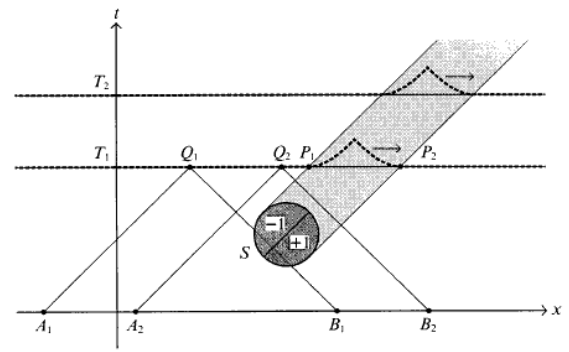
\includegraphics[width=0.6\textwidth]{prob23.png}
\end{figure}
\end{proof}
\begin{problem}
(Equipartition of energy) Let $u$ solve the initial-value problem for the wave equation in one dimension:
\[\begin{cases}u_{tt}-u_{xx}=0&\quad\text{in }\mr\times(0,\infty)\\
	u=g,u_t=h&\quad\text{on }\mr\times\{t=0\}.\end{cases}\]
Suppose $g,h$ have compact support. The \textit{kinetic energy} is $k(t):=\dis\frac{1}{2} \int_{-\infty}^{\infty}u_t^2(x,t)\dif x$ and the \textit{potential energy} is $p(t):=\dis\frac{1}{2}\int_{-\infty}^{\infty}u_x^2(x,t)\dif x$. Prove\\
(a) $k(t)+p(t)$ is constant in $t$,\\
(b) $k(t)=p(t)$ for all large enough times $t$.
\end{problem}
\begin{proof}
(a) Take derivative of $k(t)$ and $p(t)$, we have\[\begin{gathered}
	k_t(t)=\frac{\ptl}{\ptl t}\frac{1}{2} \int_{-\infty}^{\infty}u_t^2(x,t)\dif x=\int_{-\infty}^{\infty}u_t\cdot u_{tt}\dif x,\\
	p_t(t)=\frac{\ptl}{\ptl t}\frac{1}{2}\int_{-\infty}^{\infty}u_x^2(x,t)\dif x=\int_ {-\infty}^{\infty}u_x\cdot u_{xt}\dif x=-\int_{-\infty}^{\infty}u_{xx}\cdot u_t\dif x.
\end{gathered}\]
Hence $k_t(t)+p_t(t)=\dis\int_{-\infty}^{\infty}u_t\cdot(u_{tt}-u_{xx})\dif x=0$ which implies that $k(t)+p(t)$ is constant over $t$.\\
(b) D'Alembert's formula gives us the explicit solution \[\frac{1}{2}[g(x+t)+g(x-t)]+\frac{1}{2} \int_{x-t}^{x+t}h(y)\dif y\] and thus
\[\begin{aligned}
	&u_t=\frac{1}{2}[g^{\prime}(x+t)-g^{\prime}(x-t)]+\frac{1}{2}[h(x+t)+h(x-t)],\\
	&u_x=\frac{1}{2}[g^{\prime}(x+t)+g^{\prime}(x-t)]+\frac{1}{2}[h(x+t)-h(x-t)].
\end{aligned}\]
Since both $g$ and $h$ are compactly supported, for large enough $t$ we have $u_t^2=u_x^2$. Therefore $k(t)-p(t)=0$, that is $k(t)=p(t)$ for all large enough times $t$.
\end{proof}


\newpage
\section{Transform Methods}
\subsection{Fourier transform}
In this section, all functions are complex-valued.

\noindent\textcolor{blue}{Definitions and properties.}
\begin{definition}
If $u \in L^1(\mr^n)$, we define its \emph{Fourier transform} $\mathcal{F}u=\hat{u}$ by\[
\hat{u}(y):=\frac{1}{(2\pi)^{n/2}}\int_{\mr^n}\e^{-\i x\cdot y}u(x)\dif x(y\in\mr^n)\]
and its \emph{inverse Fourier transform} $\mathcal{F}^{-1}u=\check{u}$ by\[\check{u}(y)
:=\frac{1}{(2\pi)^{n/2}}\int_{\mr^n}\e^{\i x\cdot y}u(x)\dif x(y\in\mr^n).\]
\end{definition}
\begin{remark}
Since $|\e^{ \pm\i x\cdot y}|=1$ and $u\in L^1(\mr^n)$, these integrals converge for each $y\in\mr^n$.
\end{remark}
\begin{theorem}\label{thm3.1}
(Plancherel's Theorem). Assume $u\in L^1(\mr^n)\cap L^2(\mr^n)$.
Then $\hat{u},\check{u}\in L^2(\mr^n)$ and \[\|\hat{u}\|_{L^2(\mr^n)}=
\|\check{u}\|_{L^2(\mr^n)}=\|u\|_{L^2(\mr^n)}.\tag{69}\label{69}\]
\end{theorem}
\begin{proof}
It is not our concern. Refer to p188 of the book.
\end{proof}
\begin{lemma}
(Basic properties of Fourier transform).\\
\textup{(i)} (Inverse) $(\mathcal{F}^{-1}u)(x)=(\mathcal{F}u)(-x)$;\\
\textup{(ii)} (Scaling) $(\mathcal{F}u(\lambda x))(\xi)=\lambda^{-n}(\mathcal{F}u(x)) (\xi/\lambda)$;\\
\textup{(iii)} (Translation) $(\mathcal{F}f(x-h))(\xi)=\e^{-\i\xi h}(\mathcal{F}f(x))(\xi)$; \\ 
\textup{(iv)} (Convolution) $(\mathcal{F}(f*g))(x)=2\pi^{n/2}(\mathcal{F}f)(x) (\mathcal{F}g)(x)$;\\
\textup{(v)} (Modulation) $(\mathcal{F}(\e^{\i hx}f(x)))(\xi)=(\mathcal{F}f)(\xi-h)$;\\
\textup{(vi)} (Conjugation) $(\mathcal{F}\bar{f})(x)=\overline{(\mathcal{F}f)(-x)}$.
\end{lemma}
\begin{proof}
It is so trivial that we only prove (ii), (iii) and (vi), leaving the rest as exercises.\\
(ii) In fact,\[
\begin{aligned}
	(\mathcal{F}u(\lambda x))(\xi)&=\frac{1}{(2\pi)^{n/2}}\int_{\mr^n}\e^{-\i\xi x}u(\lambda x)\dif x\\
	&=\frac{1}{(2\pi)^{n/2}}\mathop{\lambda^{-n}}_{\text{Jacobian}}\int_{\mr^n} \e^{-\i\frac{\xi}{\lambda}y}u(y)\dif y=\lambda^{-n}(\mathcal{F}u(x))(\xi/\lambda).
\end{aligned}\]
(iii) In fact, \[\begin{aligned}
	(\mathcal{F}f(x-h))(\xi)&=\frac{1}{(2\pi)^{n/2}}\int_{\mr^n}\e^{-\i\xi x}f(x-h)\dif x\\
	&=\frac{1}{(2\pi)^{n/2}}\int_{\mr^n}\e^{-\i\xi(y+h)}f(y)\dif y=\e^{-\i\xi h}(\mathcal{F}f(x))(\xi).
\end{aligned}\]
(vi) In fact, \[\overline{(\mathcal{F}f)(\xi)}=\overline{\int_{\mr^n}\e^{-\i\xi x}f(x)\dif x}=\int_{\mr^n}\e^{\i\xi x}\overline{f(x)}\dif x,\]and replacing $\xi$ by $-\xi$, we have \[\overline{(\mathcal{F}f)(-\xi)}=\int_{\mr^n}\e^{-\i\xi x}\overline{f(x)}\dif x=(\mathcal{F}\bar{f})(\xi).\]
\end{proof}
\begin{theorem}\label{thm3.2}
(Properties of Fourier transform). Assume $u,v\in L^2(\mr^n)$.
Then\\
\textup{(i)} $\dis\int_{\mr^n}u\bar{v}\dif x=\int_{\mr^n}\hat{u}\overline{\hat{v}}\dif y$.\\
\textup{(ii)} $(D^\alpha u)\,{\hat{}}=(\i y)^\alpha\hat{u} $ for each multiindex $\alpha$ such that $D^\alpha u\in L^2(\mr^n)$.\\
\textup{(iii)} If $u,v\in L^1(\mr^n)\cap L^2(\mr^n)$, then $(u*v)\,{\hat{}}=(2\pi)^{n/2}\hat{u}\hat{v}$.\\
\textup{(iv)} Furthermore, $u=(\hat{u})\,\check{}$.
\end{theorem}
\begin{proof}
Another good chance to practice analytical skills. Here we list some hints.\\
(i) By Theorem \ref{thm3.1}, we have $\|u+\alpha v\|_{L^2}^2=\|\widehat{u+\alpha v}\|_{L^2}^2$. Rewriting with inner product (of $L^2$ space), and expanding the equation, we obtain $\langle u,\alpha v\rangle+\langle\alpha v,u\rangle=\langle\hat{u},\alpha\hat{v} \rangle+\langle\alpha\hat{v},\hat{u}\rangle$. Set $\alpha=1$ and $\i$, and rewrite the inner product as integrals, to obtain $\re u\bar{v}=\re\hat{u}\bar{\hat{v}}$ and $\ima u\bar{v} =\ima\hat{u}\bar{\hat{v}}$. Adding them together implies the result.\\
(ii) First assume that $u$ is smooth and has compact support. Integrate by parts, and the $\ptl\mr^n$ term vanishes since $u$ has compact support. In this process the differential operator is transferred onto $\e^{-\i x\xi}$ through $|\alpha|$ times of integration by parts, i.e. \[(D^\alpha u)\,\hat{}\,(\xi)=\frac{1}{(2\pi)^{n/2}}\int_{\mr^n}\e^{-\i x\cdot\xi} D^\alpha u(x)\dif x=\frac{(-1)^{|\alpha|}}{(2\pi)^{n/2}}\int_{\mr^n}D_x^\alpha(\e^{-\i x\cdot\xi})u(x)\dif x.\]Then calculating the derivative produces another $(-1)^{|\alpha|}$, and the result follows in this case. By approximation the same formula is true if $D^\alpha u\in L^2(\mr^n)$.\\
(iii) Direct computations. Notice the variables and the order of integration.\\
(iv) First calculate that, for $u,v\in L^1(\mr^n)\cap L^2(\mr^n)$, \[\int_{\mr^n}\check{u}v\dif x=\frac{1}{(2\pi)^{n/2}}\int_{\mr^n}\int_{\mr^n}\e^{\i x\cdot y}u(y)v(x)\dif x\dif y=\int_{\mr^n}u\check{v}\dif x.\]Also $\check{v}=\overline{(\bar{v})\,\check{}}$, and so we can employ (i) to conclude that \[\int
_{\mr^n}(\hat{u})\,\check{}v\dif x=\int_{\mr^n}uv\dif x\]for all $v\in L^2(\mr^n)$.
\end{proof}

\noindent\textcolor{blue}{Applications.} The Fourier transform $\mathcal{F}$ is an especially powerful technique for studying linear, constant-coefficient partial differential equations. Below are a few examples, including some familiar equations.
\begin{example}
(Bessel potentials). We investigate first the PDE\[-\Delta u+u=f\quad\text{in }\mr^n,\] where $f\in L^2(\mr^n)$. We take the Fourier transform, recalling Theorem \ref{thm3.2}(ii) to obtain\[\mathcal{F}(-\Delta u)(y)=\mathcal{F}\left(\sum_{j=1}^nu_{y_iy_i}\right) (y),\]and so\[(1+|y|^2)\hat{u}(y)=\hat{f}(y)(y\in\mr^n).\]Thus \[\hat{u}=\frac{\hat{f}}{1+|y|^2}\implies u=\mathcal{F}^{-1} \left(\frac{\hat{f}}{1+|y|^2}\right).\tag{70}\label{70}\]Now the only real problem is to rewrite the right-hand side of (\ref{70}) into a more explicit form. Invoking Theorem \ref{thm3.2}(iii), we set $B(x)=\mathcal{F}^{-1}\left(\frac{1}{1+|y|^2}\right)(x)$, and then $\hat{u}=\hat{f}\hat{B}$, i.e. $u=(2\pi)^{-n/2}(f*B)(x)$. Now we compute
\[\begin{aligned}
	B(x)&=\frac{1}{(2\pi)^{n/2}}\int_{\mr^n}\e^{\i x y}\frac{1}{1+|y|^2}\dif y=\frac{1}{(2\pi)^{n/2}}\int_{\mr^n}\int_0^\infty\e^{\i xy}\e^{-t}\e^{-|y|^2t}\dif t\dif y\\
	&=\frac{1}{(2\pi)^{n/2}}\int_0^\infty\e^{-t}\left(\int_{\mr^n}\e^{\i xy}\e^{-t|y|^2} \dif y\right)\dif t=\frac{1}{(2\pi)^{n/2}}\int_0^\infty\e^{-t}\left(\frac{\pi}{t}\right) ^{n/2}\e^{-\frac{|x|^2}{4t}}\dif t\\
	&=\frac{1}{2^{n/2}}\int_0^\infty\e^{-t}t^{-n/2}\e^{-|x|^2/4t}\dif t,
\end{aligned}\]where the second equality is because \[\frac{1}{a}=\int_0^\infty\e^{-at}\dif t(a>0)\implies\frac{1}{1+|y|^2}=\int_0^\infty\e^{-(1+|y|^2)t}\dif t,\]and the forth equality is due to \[\int_{\mr^n}\e^{\i xy-t|y|^2}\dif y=\left(\frac{\pi}{t}\right)^{n/2} \e^{-\frac{|x|^2}{4t}}.\]($B$ is called a \emph{Bessel potential}.) Hence\[u(x)=\frac{1}{(4\pi)^{n/2}}\int_0^\infty\int_{\mr^n}
\frac{\e^{-t-\frac{|x-y|^2}{4 t}}}{t^{n/2}}f(y)\dif y\dif t(x\in\mr^n).\]
\end{example}
\begin{example}
(Heat equation). Consider again the initial-value problem for the heat equation 
\[\left\{\begin{aligned}
	u_t-\Delta u=0&\quad\text{in } \mr^n\times(0,\infty)\\
	u=g&\quad\text{on } \mr^n\times\{t=0\}.
\end{aligned}\right.\]Take Fourier transform (in $x$) to obtain \[\left\{\begin{aligned}
\hat{u}_t+|y|^2\hat{u}=0&\quad\text{for } t>0\\
\hat{u}=\hat{g}&\quad\text{for } t=0.
\end{aligned}\right.\]Solving the ODE yields $\hat{u}=\e^{-t|y|^2}\hat{g}$. Set $F(x)=\mathcal{F}^{-1}(\e^{-t|y|^2})(x)$, and so $\hat{u}=\hat{F}\hat{g}$. Thus \[u=
\frac{g *F}{(2\pi)^{n/2}}.\]But then \[F=\frac{1}{(2\pi)^{n/2}}\int_{\mr^n}
\e^{\i x\cdot y-t|y|^2}\dif y=\frac{1}{(2t)^{n/2}} \e^{-\frac{|x|^2}{4t}}\](the details are left as an exercise). Thus \[\tag{71}\label{71}u(x,t)=\frac{1}{(4\pi t)^{n/2}}\int_{\mr^n}
\e^{-\frac{|x-y|^2}{4t}}g(y)\dif y(x\in\mr^n, t>0),\]in agreement with (\ref{35}). Here we come to an estimate $|u(x,t)|\leq\frac{1}{(4\pi t)^{n/2}}\|g\|_{L^1(\mr^n)}$ by the way.
\end{example}
\begin{example}
(Fundamental solution of Schrödinger's equation). Let us next look at the initial-value problem for Schrödinger's equation \[\left\{\begin{aligned}
	\i u_t+\Delta u=0&\quad\text{in } \mr^n\times(0,\infty)\\
	u=g&\quad\text{on } \mr^n\times\{t=0\}
\end{aligned}\right.\]Here $u$ and $g$ are complex-valued. If we formally replace $t$ by $\i t$ on the right-hand side of (\ref{71}), we obtain the formula\[\tag{72}\label{72}u(x,t)= \frac{1}{(4\pi\i t)^{n/2}}\int_{\mr^n}\e^{\frac{\i|x-y|^2}{4t}}g(y)\dif y(x\in\mr^n, t>0),\]where we interpret $\i^{\frac{1}{2}}$ as $\e^{\frac{\i\pi}{4}}$. This expression clearly makes sense for all times $t>0$, provided $g\in L^1(\mr^n)$.

Now we go back and take Fourier transform to obtain \[\left\{\begin{array}{l}
	{\color{red}\i}\hat{u}_t{\color{red}-}|y|^2\hat{u}(y,t)=0(t>0)\\
	\hat{u}(y,t=0)=\hat{g}(y).
\end{array}\right.\]Solve the ODE to obtain $\hat{u}(y,t)=\e^{-{\color{red}\i}t|y|^2} \hat{g}(y)$. The remaining steps are all the same as the previous example, and this is where (\ref{72}) comes from.

We again estimate that $|u(x,t)|\leq\frac{1}{(4\pi t)^{n/2}}\|g\|_{L^1(\mr^n)}$, i.e. $\|u\|_{L^\infty}\lesssim t^{-\frac{n}{2}}\|g\|_{L^1}$. Indeed, since $|(4\pi\i t)^{-n/2}|\leq(4\pi t)^{-n/2}$ and $\left|\e^{\frac{\i|x-y|^2}{4t}}\right|=1(t>0)$, we have \[
|u(x,t)|\leq\frac{1}{(4\pi t)^{n/2}}\int_{\mr^n}g(y)\dif y=Ct^{-n/2}\|g\|_{L^1(\mr^n)}. \]Rewrite formula (\ref{72}) as\[u(x,t)=\frac{\e^{\i|x|^2/4t}}{(4\pi\i t)^{n/2}}\int_ {\mr^n}\e^{-\i xy/2t}\e^{\i|y|^2/4t}g(y)\dif y,\]and we can check as in Theorem \ref{thm3.1} that if $g\in L^1(\mr^n)\cap L^2(\mr^n)$, then $\|u\|_{L^2(\mr^n)} =\|g\|_{L^2(\mr^n)}$. In fact, for the heat equation, we have\[\|u\|_{L^2}=\|\hat{u}\|_
{L^2}=\|e^{-t|y|^2}\hat{g}(y)\|_{L^2}\leq\|\hat{g}\|_{L^2}=\|g\|_{L^2}(t>0);\] but for Schrödinger's equation, we have\[\|u\|_{L^2}=\|\hat{u}\|_{L^2}=\|e^{-\i t|y|^2}\hat{g}(y)\|
_{L^2}=\|\hat{g}\|_{L^2}=\|g\|_{L^2}(t>0).\]
\end{example}
\begin{remark}
We call\[\Psi(x,t):=\frac{1}{(4\pi\i t)^{n/2}}\e^{\frac{\i|x|^2}{4t}}(x\in\mr^n,t\neq0)\] the fundamental solution of Schrödinger's equation. Note that formula (\ref{72}), $u=g*\Psi$, makes sense for all times $t\neq0$, even $t<0$.
\end{remark}
\begin{example}
(Wave equation). We next analyze the initial-value problem for the wave equation \[
\left\{\begin{aligned}
	u_{tt}-\Delta u=0&\quad\text{in } \mr^n\times(0,\infty)\\
	u=g,u_t=h&\quad\text{on } \mr^n\times\{t=0\},
\end{aligned}\right.\]where for simplicity we suppose the initial velocity to be zero. Take Fourier transform as before and then \[\left\{\begin{aligned}
\hat{u}_{tt}+|y|^2\hat{u}=0&\quad\text{for } t>0\\
\hat{u}=\hat{g},\hat{u}_t=\hat{h}&\quad\text{for } t=0.
\end{aligned}\right.\]This time we will separately study these two initial-value problems:
\[\left\{\begin{aligned}
	u_{tt}-\Delta u=0&\quad\text{in } \mr^n\times(0,\infty)\\
	u=g,u_t=0&\quad\text{on } \mr^n\times\{t=0\},
\end{aligned}\right.\quad\left\{\begin{aligned}
	u_{tt}-\Delta u=0&\quad\text{in } \mr^n\times(0,\infty)\\
	u=0,u_t=h&\quad\text{on } \mr^n\times\{t=0\}.
\end{aligned}\right.\]For the former, its Fourier transform reads \[\left\{\begin{array}{l}
\hat{u}_{tt}+|y|^2\hat{u}=0(t>0)\\
\hat{u}(y,t=0)=\hat{g}(y)\\
\hat{u}_t(y,t=0)=0.
\end{array}\right.\]Solve the ODE to obtain a fundamental set of solutions $e^{\i t|y|}$ and $e^{-\i t|y|}$. Use the initial conditions to write \[\left\{\begin{array}{l}a(y)+b(y)=\hat{g}(y)\\ \i|y|a(y)-\i|y|b(y)=0,\end{array}\right.\] and then $\hat{u}(y,t)=\frac{1}{2}(\e^{\i t|y|}+\e^{-\i t|y|})\hat{g}(y)=\cos(t|y|)\hat{g} (y)$. Now do the inverse Fourier transform and we get\[u(x,t)=\frac{1}{(2\pi)^{n/2}}\int_
{\mr^n}\e^{\i xy}\cos(t|y|)\hat{g}(y)\dif y.\]

We turn our attention to the latter initial-value problem. This time\[\left\{\begin{array}{l}
	\hat{u}_{tt}+|y|^2\hat{u}=0(t>0)\\
	\hat{u}(y,t=0)=0\\
	\hat{u}_t(y,t=0)=\hat{h}(y),
\end{array}\right.\]and the solution of this ODE is \[\hat{u}(y,t)=\frac{\hat{h}(y)}{2\i|y|} \e^{\i t|y|}-\frac{\hat{h}(y)}{2\i|y|}\e^{-\i t|y|}=\frac{\sin(t|y|)}{|y|}\hat{h}(y).\]Hence\[
u(x,t)=\frac{1}{(2\pi)^{n/2}}\int_{\mr^n}\e^{\i xy}\frac{\sin t|y|}{|y|}h(y)\dif y.\]We will next prove that this equals exactly \[\begin{cases}
\dis\frac{1}{2}\int_{x-t}^{x+t}h(y)\dif y,&n=1,\\[6pt]
t\dis\dashint_{\ptl B(x,t)}h(y)\dif S(y),&n=3.
\end{cases}\]

When $n=1$, we have\[\frac{\sin|y|}{|y|}\xlongequal{y\in\mr^1}\frac{\sin y}
{y}=\frac{1}{2}\int_{-1}^1\e^{-\i xy}\dif x\implies\frac{\sin t|y|}{|y|}=\frac{t}{2} \int_{-1}^1\e^{-\i zty}\dif z,\] and thus\[\begin{aligned}
u(x,t)&=\frac{1}{(2\pi)^{1/2}}\int_\mr\e^{\i xy}\frac{t}{2}\int_{-1}^1\e^{-\i zty}\dif z\hat{h}(y)\dif y\\
&=\frac{1}{2}\mathop{\int_{-1}^1}_{(z)}t\mathop{\int_\mr}_{(y)}\e^{\i xy-\i zty}\mathop{\int_\mr}_{(\eta)}\e^{\i y\eta}h(\eta)\dif\eta\dif y\dif z\cdot\frac{1} {2\pi}\\
&=\frac{1}{2}\mathop{\int_{-1}^1}_{(z)}t\mathop{\int_\mr}_{(\eta)}\mathop{\int_\mr}_{(y)}\frac{1}{2\pi}\e^{-i(\eta+zt-x)y}\dif y\,h(\eta)\dif\eta\dif z\\
&=\frac{1}{2}\mathop{\int_{-1}^1}_{(z)}t\mathop{\int_{-\infty}^\infty}_{(\eta)}\delta(\eta+zt-x)h(\eta)\dif\eta\dif z\quad(\text{since } \int_{-\infty}^\infty\e^{-\i xy}\dif x=2\pi\delta(y))\\
&=\frac{1}{2}\int_{-1}^1th(x-tz)\dif z\quad(\text{since } \eta+zt-x=0\implies\eta=x-zt)\\
&=\frac{1}{2}\int_{x-t}^{x+t}h(y)\dif y.\quad(\text{letting } y=x-tz)
\end{aligned}\]This coincides with d'Alembert's formula (\ref{50}).

For the case $n=3$, first note that \[\int_{|x|=1}\e^{-\i\xi x}\dif S(x)=4\pi\frac{\sin|\xi|} {|\xi|},\]and by substituting we have \[\frac{\sin t|\xi|}{|\xi|}=\frac{1}{t|\ptl B(0,1)|}
\int_{\ptl B(0,t)}\e^{-\i y \xi}\dif S(y).\]Consequently, \[\begin{aligned}
u(x,t)&=\frac{1}{(2\pi)^{3/2}}\int_{\mr^3}\e^{\i xy}\frac{\sin t|y|}{|y|}\hat{h}(y)\dif y\\
&=\frac{1}{(2\pi)^{3/2}}\int_{\mr^3}\e^{\i xy}\frac{1}{t|\ptl B(0,1)|}\int_{\ptl B(0,t)} \e^{-\i zy}\dif S(z)\frac{1}{(2\pi)^{3/2}}\int_{\mr^3}\e^{\i\xi y}h(\xi)\dif\xi\dif y\\
&=\frac{1}{(2\pi)^3}\frac{1}{t|\ptl B(0,1)|}\int_{\ptl B(0,t)}\int_{\mr^3}\int_{\mr^3}\e ^{-\i y(z+\xi-x)}\dif y\,h(\xi)\dif\xi\dif S(z)\\
&=\frac{1}{t|\ptl B(0,1)|}\frac{1}{(2\pi)^3}\int_{\ptl B(0,t)}\int_{\mr^3}(2\pi)^3\delta (z+\xi-x)h(\xi)\dif\xi\dif S(z)\\
&=\frac{t}{t^2|\ptl B(0,1)|}\int_{\ptl B(0,t)}h(x-z)\dif S(z)\quad(\text{since } z+\xi-x=0\implies\xi=x-z)\\
&=t\dashint_{\ptl B(x,t)}h(y)\dif S(y).
\end{aligned}\]
\end{example}
\begin{example}
(Transport equation). At the end of our course, we return to the first PDE we've met, and also probably the easiest example in this chapter. Consider the transport equation\[
\left\{\begin{aligned}
	u_t+b\cdot Du=0&\quad\text{in } \mr^n\times(0,\infty)\\
	u=g&\quad\text{on } \mr^n\times\{t=0\},
\end{aligned}\right.\]and take Fourier transform as usual. This yields \[\left\{\begin{aligned}
\hat{u}_t+b\cdot\i y\cdot\hat{u}=0&\quad\text{in } \mr^n\times(0,\infty)\\
\hat{u}=\hat{g}&\quad\text{on } \mr^n\times\{t=0\}.
\end{aligned}\right.\]Solve the ODE to obtain $\hat{u}(y,t)=\e^{-\i byt}\hat{g}(y)$. Hence \[u(x,t)=\frac{1}{(2\pi)^{n/2}}\int_{\mr^n}\e^{\i xy}\e^{-\i byt}\hat{g}(y)\dif y= \frac{1}{(2\pi)^{n/2}}\int_{\mr^n}\e^{\i(x-bt)y}\hat{g}(y)\dif y=g(x-bt).\]
\end{example}


\newpage
\begin{appendices}
\addcontentsline{toc}{section}{Appendices}
\begin{center}
\Large{\textbf{APPENDICES}}
\end{center}
	
\section{Notations}
\subsection*{A.1\quad Geometric notation.}\label{app.a.1}
\begin{enumerate}
\item $e_i=(0,\cdots,0,1,\cdots,0)=i^{\text{th}}$ standard coordinate vector of $\mr^n$.
\item $\mr_+^n=\{x=(x_1,\cdots,x_n)\in\mr^n\mid x_n>0\}=$ open upper half-space.
\item A typical point in $\mr^{n+1}$ will often be denoted as $(x,t)=(x_1,\cdots,x_n,t)$, and we usually interpret $t=x_{n+1}=$ time.
\item $U,V$, and $W$ usually denote open subsets of $\mr^n$. We write\[V\subset\subset U\]if $V\subset\bar{V}\subset U$ and $\bar{V}$ is compact, and say $V$ is compactly contained in $U$.
\item For open and bounded $U$, $U_T=U\times(0,T]=$ the parabolic cylinder, $\Gamma_T=\bar{U}_T-U_T=$ parabolic boundary of $U_T$.
\item $B^0(x,r)=\{y\in\mr^n\mid|x-y|<r\}=$ open ball in $\mr^n$ with center $x$ and radius $r>0$.
\item $B(x,r)=$ closed ball with center $x$, radius $r>0$.
\item $\alpha(n)=\dfrac{\pi^{n/2}}{\Gamma\left(\frac{n}{2}+1\right)}=$ volume of unit ball $B(0,1)$ in $\mr^n$.\\[5pt]
$n\alpha(n)=$ surface area of unit sphere $\ptl B(0,1)$ in $\mr^n$ (note that its dimension is $n-1$).\\[3pt]
Hence the volume of $B(0,r)$ in $\mr^n$ is $r^n\alpha(n)$, and the surface area of it is $n\alpha(n)r^{n-1}$.
\item If $a=(a_1,\cdots,a_n)$ and $b=(b_1,\cdots,b_n)$ belong to $\mr^n$,
\[a\cdot b=\sum_{i=1}^na_ib_i,|a|=\left(\sum_{i=1}^na_i^2\right)^{\frac{1}{2}}.\]
\end{enumerate}

\subsection*{A.2\quad Notation for functions, derivatives and function spaces.}
\begin{enumerate}
\item If $u:U\to\mr$, we write\[u(x)=u(x_1,\cdots,x_n)(x\in U).\]
We say $u$ is smooth provided $u$ is infinitely differentiable. The support of a function $u$ is denoted $\spt u$.
\item If $\mathbf{u}:U\to\mr^m$, we write\[\mathbf{u}(x)=(u^1(x),\cdots,u^m(x))(x\in U).\]The function $u^k$ is the $k^{\text{th}}$ component of $\mathbf{u},k=1,\cdots,m$.
\item $\dis\dashint_{B(x, r)}f\dif y=\frac{1}{\alpha(n) r^n} \int_{B(x, r)} f d y=$ average of $f$ over the ball $B(x,r)$ \\[6pt] and\\[6pt]
$\dis\dashint_{\ptl B(x,r)}f\dif S=\frac{1}{n\alpha(n)r^{n-1}}\int_{\ptl B(x,r)}f\dif S=$ average of $f$ over the sphere $\ptl B(x,r)$.
\item The convolution of the functions $f, g$ is denoted $f*g$.
\item Assume $u:U\to\mr,x\in U$, the same below. $u_{x_i}=\dfrac{\ptl u}{\ptl x_i}=\limls_{h\to0}\dfrac{u(x+he_i)-u(x)}{h}$, provided this limit exists. Similarly, $\dfrac{\ptl^2u}{\ptl x_i\ptl x_j}=u_{x_ix_j}, \dfrac{\ptl^3u}{\ptl x_i\ptl x_j\ptl x_k}=u_{x_ix_jx_k}$, etc.
\item Multiindex Notation:\\
(a) A vector of the form $\alpha=(\alpha_1,\cdots,\alpha_n)$, where each component $\alpha_i$ is a nonnegative integer, is called a multiindex of order
\[|\alpha|=\alpha_1+\cdots+\alpha_n.\]
(b) Given a multiindex $\alpha$, define
\[D^\alpha u(x):=\frac{\ptl^{|\alpha|} u(x)}{\ptl x_1^{\alpha_1}\cdots\ptl x_n^{\alpha_n}}=\ptl_{x_1}^{\alpha_1}\cdots\ptl_{x_n}^{\alpha_n}u.\]
(c) If $k$ is a nonnegative integer,\[D^ku(x):=\{D^\alpha u(x)\mid|\alpha|=k\},\]
the set of all partial derivatives of order $k$. Assigning some ordering to the various partial derivatives, we can also regard $D^ku(x)$ as a point in $\mr^{n^k}$.
\[|D^k u|=\left(\sum_{|\alpha|=k}|D^\alpha u|^2\right)^{1/2}.\tag{d}\]
(e) Special Cases: If $k=1$, we regard the elements of $Du$ as being arranged in a vector:
\[Du=(u_{x_1},\cdots,u_{x_n})=\text{~gradient vector}.\]
If $k=2$, we regard the elements of $D^2 u$ as being arranged in a matrix:
\[D^2u=\begin{pmatrix}
	\frac{\ptl^2 u}{\ptl x_1^2}&\cdots&\frac{\ptl^2 u}{\ptl x_1\ptl x_n}\\
	&\ddots&\\
	\frac{\ptl^2 u}{\ptl x_n\ptl x_1}&\cdots&\frac{\ptl^2 u}{\ptl x_n^2}
\end{pmatrix}_{n\times n}=\text{~Hessian matrix}.\]
\item $\dis\Delta u=\sum_{i=1}^nu_{x_ix_i}=\tr(D^2u)=$ Laplacian of $u$.
\item We sometimes employ a subscript attached to the symbols $D,D^2$, etc. to denote the variables being differentiated, such as $D_xu=(u_{x_1},\cdots,u_{x_n}),D_yu=(u_{y_1},\cdots,u_{y_m})$.
\item $C(\bar{U})=\{u \in C(U) \mid u \text{~uniformly continuous} \}$\\
$C^k(\bar{U})=\{u \in C^k(U) \mid D^\alpha u \text{~is uniformly continuous for all} |\alpha| \leq k\}$.\\
Thus if $u\in C^k(\bar{U})$, then $D^\alpha u$ continuously extends to $\bar{U}$ for each multiindex $\alpha,|\alpha|\leq k$.
\item $C^\infty(U)=\{u:U\to\mr\mid u \text{~infinitely differentiable}\}=\dis\bigcap_{k=0}^{\infty}C^k(U),C^\infty(\bar{U})=\bigcap_{k=0}^{\infty}C^k(\bar{U})$.
\item $C_c(U),C_c^k(U)$, etc. denote these functions in $C(U),C^k(U)$, etc. with compact support.
\item The definitions of $L^p(U)$ and $L^\infty(U)$ are the same as those in real analysis.
\item It is occasionally useful to introduce spaces of functions with differing smoothness in the $x$- and $t$- variables, although there is no standard notation for such spaces. We will for this book write
\[C_1^2(U_T)=\{u: U_T\to\mr\mid u,D_xu,D_x^2 u,u_t\in C(U_T)\}.\]
In particular, if $u\in C_1^2(U_T)$, then $u,D_xu$, etc. are continuous up to the top $U \times\{t=T\}$.
\end{enumerate}

\newpage
\section{Calculus Facts}
\subsection*{B.1\quad Boundaries.}
Let $U\subset\mr^n$ be open and bounded, $k\in\{1,2,\cdots\}$.
\begin{definition}
We say $\ptl U$ is $C^k$ if for each point $x^0\in\ptl U$ there exist $r>0$ and a $C^k$ function $\gamma:\mr^{n-1}\to\mr$ such that- upon relabeling and reorienting the coordinates axes if necessary- we have
\[U\cap B(x^0,r)=\{x\in B(x^0,r)\mid x_n>\gamma(x_1,\cdots,x_{n-1})\}.\]
Likewise, $\ptl U$ is $C^\infty$ if $\ptl U$ is $C^k$ for $k=1,2,\cdots$, and $\ptl U$ is analytic if the mapping $\gamma$ is analytic.
\end{definition}
\begin{definition}\label{ounv}
\textup{(i)} If $\ptl U$ is $C^1$, then along $\ptl U$ is defined the outward pointing unit normal vector field\[\bm{\nu}=(\nu^1,\cdots,\nu^n).\]
The unit normal at any point $x^0\in\ptl U$ is $\bm{\nu}(x^0)=\nu=(\nu_1,\cdots,\nu_n)$.\\
\textup{(ii)} Let $u\in C^1(\bar{U})$. We call\[\frac{\ptl u}{\ptl\nu}:=\bm{\nu}\cdot Du\]the (outward) normal derivative of $u$.
\end{definition}
\subsection*{B.2\quad Gauss-Green theorem.}
In this section we assume $U$ is a bounded, open subset of $\mr^n$, and $\ptl U$ is $C^1$.
\begin{theorem}\label{GGt}
(Gauss-Green Theorem) Suppose $u\in C^1(\bar{U})$. Then
\[\int_Uu_{x_i}\dif x=\int_{\ptl U}u\nu^i\dif S(i=1,\cdots,n).\tag{B1}\]
\end{theorem}
\begin{theorem}
(Integration-by-parts formula) Let $u,v\in C^1(\bar{U})$. Then
\[\int_Uu_{x_i}v\dif x=-\int_Uuv_{x_i}\dif x+\int_{\ptl U}uv\nu^i\dif S(i=1,\cdots,n).\label{B2}\tag{B2}\]
\end{theorem}
\begin{proof}
Apply Theorem B.1 to $uv$.
\end{proof}
\begin{theorem}
	\label{thmb3}
(Green's formulas) Let $u,v\in C^2(\bar{U})$. Then\\
\textup{(i)} $\dis\int_U\Delta u\dif x=\int_{\ptl U} \frac{\ptl u}{\ptl\nu}\dif S$,\\
\textup{(ii)} $\dis\int_UDv\cdot Du\dif x=-\int_Uu\Delta v\dif x+\int_{\ptl U}\frac{\ptl v}{\ptl \nu}u\dif S$,\\[6pt]
\textup{(iii)} $\dis\int_Uu\Delta v-v\Delta u\dif x=\int_{\ptl U}u\frac{\ptl v}{\ptl\nu}-v\frac{\ptl u}{\ptl\nu}\dif S$.
\end{theorem}
\begin{proof}
Using (\ref{B2}), with $u_{x_i}$ in place of $u$ and $v\equiv1$, we see
\[\int_Uu_{x_ix_i}\dif x=\int_{\ptl U}u_{x_i}\nu^i\dif S.\]Sum $i=1,\cdots,n$ to establish (i).

To derive (ii), we employ (\ref{B2}) with $v=u_{x_i}$. Write (ii) with $u$ and $v$ interchanged and then subtract, to obtain (iii).
\end{proof}

\subsection*{B.3\quad Polar coordinates.}\label{polar}
Next we convert $n$-dimensional integrals into integrals over spheres.
\begin{theorem}\label{b4}
(Polar coordinates)\\\textup{(i)} Let $f:\mr^n\to\mr$ be continuous and summable. Then
\[\int_{\mr^n}f\dif x=\int_0^\infty\left(\int_{\ptl B(x_0,r)} f\dif S\right)\dif r\]
for each point $x_0\in\mr^n$.\\
\textup{(ii)} In particular\[\frac{\dif}{\dif r}\left(\int_{B(x_0,r)}f\dif x\right)=\int_{\ptl B(x_0,r)}f\dif S\]for each $r>0$.
\end{theorem}

\subsection*{B.4\quad Convolution and smoothing.}\label{smooth}
If $U\subset\mr^n$ is open, $\ve>0$, write $U_\ve:=\{x\in U:\operatorname{dist}(x,\ptl U)>\ve\}$.
\begin{definition}
\textup{(i)} Define $\eta\in C^\infty(\mr^n)$ by
\[\eta(x):=\begin{cases}C\exp\left(\frac{1}{|x|^2-1}\right)&\text{~if}~|x|<1\\0&\text{~if}~|x|\geq1,\end{cases}\]
the constant $C>0$ selected so that $\dis\int_{\mr^n}\eta\dif x=1$.\\[4pt]
\textup{(ii)} For each $\ve>0$, set
\[\eta_\ve(x):=\frac{1}{\ve^n}\eta\left(\frac{x}{\ve}\right).\]
\end{definition}
We call $\eta$ the \emph{standard mollifier}. Note that $\eta_\ve$ are all $C^\infty,\spt(\eta_\ve)\subset B(0,\ve)$, and\[\int_{\mr^n}\eta_\ve(x)\dif x=\int_ {\mr^n}\ve^{-n}\eta(x/\ve)\dif x\xlongequal{y=x/\ve}\int_{\mr^n}\eta(x)\dif x=1,\]i.e. $\eta_\ve$ preserves $L^1$ norm.
\begin{definition}
If $f:U\to\mr$ is locally integrable, define its mollification\[f^\ve:=\eta_\ve *f\text{~in } U_\ve.\]That is,\[f^\ve(x)=\int_U\eta_\ve(x-y)f(y)\dif y=\int_{B(0,\ve)}\eta_\ve(y)f(x-y)\dif y\]for $x\in U_\ve$.
\end{definition}
\begin{theorem}
(Properties of mollifiers)\\ \textup{(i)} $f^\ve\in C^\infty(U_\ve)$.\\
\textup{(ii)} $f^\ve\to f$ a.e. as $\ve\to0$.\\
\textup{(iii)} If $f \in C(U)$, then $f^\ve\to f$ uniformly on compact subsets of $U$.
\end{theorem}
\begin{proof}
It is not required in this course, so we just sketch the proof. For details, see pp 630-631 of the textbook.\\
(i) For $x+he_i\in U_\ve$, compute the limit of $\dfrac{f^\ve(x+he_i)-f^\ve(x)}{h}$ as $h\to0$ to show that $\dfrac{\ptl f^\ve} {\ptl x_i}(x)$ exists, and $D^\alpha f^\ve$ can be obtained similarly.\\
(ii) Use Lebesgue differentiation theorem (cf. Theorem \ref{lebdt}) to prove that $|f^\ve(x)-f(x)|\to0$ as $\ve\to0$ for a.e. $x\in U$.\\
(iii) Note that $f$ is uniformly continuous on $W$, where $V\subset\subset W\subset\subset U$ for a given $V\subset\subset U$. Then make use of (ii).
\end{proof}


\subsection*{B.5\quad Dirac $\delta$-function.}\label{Dirac}
Dirac $\delta$-function, also known as the unit impulse, is a generalized function on the real numbers, whose value is zero everywhere except at zero, and whose integral over the entire real line is equal to one. In other words, $\delta(x)=0(x\neq0)$, and $\dis\int_\mr\delta(x)\dif x=1$.

One way to rigorously capture this function is to define a measure, called Dirac measure, which accepts a subset $A$ of the real line $\mr$ as an argument, and returns $\delta(A)=1$ if $0\in A$, and $\delta(A)=0$ otherwise.

We sometimes denote a translation of $\delta(x)$ of distance $a$ by $\delta_a(x),a\in\mr$.

\subsection*{B.6\quad Measure theory.}
\begin{definition}\label{summ}
A measurable function $f$ is \emph{summable} if\[\int_{\mr^n}|f|\dif x<\infty.\]
\end{definition}
Note carefully our terminology: a measurable function is \emph{integrable} if it has an integral (which may equal $+\infty$ or $-\infty$ ) and is \emph{summable} if this integral is finite.
\begin{theorem}\label{lebdt}
(Lebesgue differentiation theorem) Let $f:\mr^n\to\mr$ be locally summable.\\
\textup{(i)} Then for a.e. point $x_0\in\mr^n$,
\[\dashint_{B(x_0,r)}f\dif x\to f(x_0)~\text{as } r\to 0.\]
\textup{(ii)} In fact, for a.e. point $x_0\in\mr^n$,
\[\dashint_{B(x_0,r)}|f(x)-f(x_0)|\dif x\to 0~\text{as } r\to0.\]
\end{theorem}

\subsection*{B.7\quad Poisson's kernel.}
Denote the Poisson's kernel for the upper space
\[\frac{2x_n}{n\alpha(n)}\frac{1}{|x-y|^n}(x\in\mr_+^n,y\in\ptl\mr_+^n)\]by $K(x,y)$, then
\begin{theorem}\label{thmb7}
$\dis\int_{\ptl\mr_+^n}K(x,y)\dif y=1$.
\end{theorem}
\begin{proof}
Write $x=(x^\prime,x_n)\in\mr_+^n$, where $x^\prime=(x_1,\cdots,x_{n-1})$. Since $y\in\ptl\mr_+^n$, we have \[\int_{\ptl\mr_+^n}K(x,y)\dif y=\frac{2x_n}{n\alpha(n)} \int_{\mr^{n-1}}\frac{1}{(|x^\prime-y^\prime|^2+x_n^2)^{n/2}}\dif y^\prime.\]Making the change of coordinates $z^\prime=\dfrac{x^\prime-y^\prime}{x_n}$ gives\[
\begin{aligned}
	\frac{2x_n}{n\alpha(n)}\int_{\mr^{n-1}}\frac{1}{(|x^\prime-y^\prime|^2+x_n^2)^{n/2}}\dif y^\prime&=\frac{2x_n}{n\alpha(n)}\int_{\mr^{n-1}}\frac{x_n^{n-1}} {x_n^n(|z^\prime|^2+1)^{n/2}}\dif z^\prime\\
	&=\frac{2}{n\alpha(n)}\int_{\mr^{n-1}}\frac{1}{(|z^\prime|^2+1)^{n/2}}\dif z^\prime.
\end{aligned}\]Now we change to polar coordinates:\[\begin{aligned}
\int_{\mr^{n-1}}\frac{1}{(|z^\prime|^2+1)^{n/2}}\dif z^\prime&=(n-1)\alpha(n-1) \int_0^\infty\frac{r^{n-2}}{(r^2+1)^{n/2}}\dif r\\
&\xlongequal{\tau=r^2}\frac{1}{2}(n-1)\alpha(n-1)\int_0^\infty\frac{\tau^{\frac{n-3}{2}}}{(\tau+1)^{n/2}}\dif\tau.
\end{aligned}\]Note that $B(x,y)=\dis\int_0^{+\infty}\frac{\tau^{x-1}}{(1+\tau)^{x+y}}\dif\tau$ (substitute $t$ with $\tau/(1+\tau)$ in $B(x,y)=\dis\int_0^1t^{x-1}(1-t)^{y-1}\dif t$), where $B$ is the Beta function. Therefore\[\int_0^\infty\frac{\tau^{\frac{n-3}{2}}}{(\tau+1)^{n/2}}\dif\tau=B\left(\frac{n-1}{2},\frac{1}{2}\right),\]and\[\int_{\ptl\mr_+^n}K(x,y)\dif y=\frac{(n-1)\alpha(n-1)}{n\alpha(n)}B\left(\frac{n-1}{2},\frac{1}{2}\right).\]Using that $\alpha(n)=\dfrac{\pi^{n/2}}{\Gamma(n/2+1)},B(x,y)=\dfrac{\Gamma(x)\Gamma(y)} {\Gamma(x+y)}$ and $\Gamma(x+1)=x\Gamma(x)$ we can verify that
\[\frac{(n-1)\alpha(n-1)}{n\alpha(n)}B\left(\frac{n-1}{2},\frac{1}{2}\right)=1.\]
\end{proof}

\subsection*{B.8\quad Duhamel's principle.}\label{Duhamel}
Duhamel's principle is a general method for obtaining solutions to nonhomogeneous linear evolution equations like the heat equation, wave equation, and vibrating plate equation. It is named after Jean-Marie Duhamel who first applied the principle to the nonhomogeneous heat equation. For linear evolution equations without spatial dependency, such as a harmonic oscillator, Duhamel's principle reduces to the method of variation of parameters technique for solving linear nonhomogeneous ODE. It is also an indispensable tool in the study of nonlinear PDE such as the Navier–Stokes equations and nonlinear Schrödinger equation where one treats the nonlinearity as an nonhomogeneity.

The philosophy underlying Duhamel's principle is that it is possible to go from solutions of the Cauchy problem (or initial value problem) to solutions of the nonhomogeneous problem. Intuitively, one can think of the nonhomogeneous problem as a set of homogeneous problems each starting afresh at a different time slice $t=t_0$. By linearity, one can add up (integrate) the resulting solutions through time $t_0$ and obtain the solution for the nonhomogeneous problem. This is the essence of Duhamel's principle.

\end{appendices}
\end{document}
